% Options for packages loaded elsewhere
\PassOptionsToPackage{unicode}{hyperref}
\PassOptionsToPackage{hyphens}{url}
%
\documentclass[
]{book}
\usepackage{amsmath,amssymb}
\usepackage{iftex}
\ifPDFTeX
  \usepackage[T1]{fontenc}
  \usepackage[utf8]{inputenc}
  \usepackage{textcomp} % provide euro and other symbols
\else % if luatex or xetex
  \usepackage{unicode-math} % this also loads fontspec
  \defaultfontfeatures{Scale=MatchLowercase}
  \defaultfontfeatures[\rmfamily]{Ligatures=TeX,Scale=1}
\fi
\usepackage{lmodern}
\ifPDFTeX\else
  % xetex/luatex font selection
\fi
% Use upquote if available, for straight quotes in verbatim environments
\IfFileExists{upquote.sty}{\usepackage{upquote}}{}
\IfFileExists{microtype.sty}{% use microtype if available
  \usepackage[]{microtype}
  \UseMicrotypeSet[protrusion]{basicmath} % disable protrusion for tt fonts
}{}
\makeatletter
\@ifundefined{KOMAClassName}{% if non-KOMA class
  \IfFileExists{parskip.sty}{%
    \usepackage{parskip}
  }{% else
    \setlength{\parindent}{0pt}
    \setlength{\parskip}{6pt plus 2pt minus 1pt}}
}{% if KOMA class
  \KOMAoptions{parskip=half}}
\makeatother
\usepackage{xcolor}
\usepackage{color}
\usepackage{fancyvrb}
\newcommand{\VerbBar}{|}
\newcommand{\VERB}{\Verb[commandchars=\\\{\}]}
\DefineVerbatimEnvironment{Highlighting}{Verbatim}{commandchars=\\\{\}}
% Add ',fontsize=\small' for more characters per line
\usepackage{framed}
\definecolor{shadecolor}{RGB}{248,248,248}
\newenvironment{Shaded}{\begin{snugshade}}{\end{snugshade}}
\newcommand{\AlertTok}[1]{\textcolor[rgb]{0.94,0.16,0.16}{#1}}
\newcommand{\AnnotationTok}[1]{\textcolor[rgb]{0.56,0.35,0.01}{\textbf{\textit{#1}}}}
\newcommand{\AttributeTok}[1]{\textcolor[rgb]{0.13,0.29,0.53}{#1}}
\newcommand{\BaseNTok}[1]{\textcolor[rgb]{0.00,0.00,0.81}{#1}}
\newcommand{\BuiltInTok}[1]{#1}
\newcommand{\CharTok}[1]{\textcolor[rgb]{0.31,0.60,0.02}{#1}}
\newcommand{\CommentTok}[1]{\textcolor[rgb]{0.56,0.35,0.01}{\textit{#1}}}
\newcommand{\CommentVarTok}[1]{\textcolor[rgb]{0.56,0.35,0.01}{\textbf{\textit{#1}}}}
\newcommand{\ConstantTok}[1]{\textcolor[rgb]{0.56,0.35,0.01}{#1}}
\newcommand{\ControlFlowTok}[1]{\textcolor[rgb]{0.13,0.29,0.53}{\textbf{#1}}}
\newcommand{\DataTypeTok}[1]{\textcolor[rgb]{0.13,0.29,0.53}{#1}}
\newcommand{\DecValTok}[1]{\textcolor[rgb]{0.00,0.00,0.81}{#1}}
\newcommand{\DocumentationTok}[1]{\textcolor[rgb]{0.56,0.35,0.01}{\textbf{\textit{#1}}}}
\newcommand{\ErrorTok}[1]{\textcolor[rgb]{0.64,0.00,0.00}{\textbf{#1}}}
\newcommand{\ExtensionTok}[1]{#1}
\newcommand{\FloatTok}[1]{\textcolor[rgb]{0.00,0.00,0.81}{#1}}
\newcommand{\FunctionTok}[1]{\textcolor[rgb]{0.13,0.29,0.53}{\textbf{#1}}}
\newcommand{\ImportTok}[1]{#1}
\newcommand{\InformationTok}[1]{\textcolor[rgb]{0.56,0.35,0.01}{\textbf{\textit{#1}}}}
\newcommand{\KeywordTok}[1]{\textcolor[rgb]{0.13,0.29,0.53}{\textbf{#1}}}
\newcommand{\NormalTok}[1]{#1}
\newcommand{\OperatorTok}[1]{\textcolor[rgb]{0.81,0.36,0.00}{\textbf{#1}}}
\newcommand{\OtherTok}[1]{\textcolor[rgb]{0.56,0.35,0.01}{#1}}
\newcommand{\PreprocessorTok}[1]{\textcolor[rgb]{0.56,0.35,0.01}{\textit{#1}}}
\newcommand{\RegionMarkerTok}[1]{#1}
\newcommand{\SpecialCharTok}[1]{\textcolor[rgb]{0.81,0.36,0.00}{\textbf{#1}}}
\newcommand{\SpecialStringTok}[1]{\textcolor[rgb]{0.31,0.60,0.02}{#1}}
\newcommand{\StringTok}[1]{\textcolor[rgb]{0.31,0.60,0.02}{#1}}
\newcommand{\VariableTok}[1]{\textcolor[rgb]{0.00,0.00,0.00}{#1}}
\newcommand{\VerbatimStringTok}[1]{\textcolor[rgb]{0.31,0.60,0.02}{#1}}
\newcommand{\WarningTok}[1]{\textcolor[rgb]{0.56,0.35,0.01}{\textbf{\textit{#1}}}}
\usepackage{longtable,booktabs,array}
\usepackage{calc} % for calculating minipage widths
% Correct order of tables after \paragraph or \subparagraph
\usepackage{etoolbox}
\makeatletter
\patchcmd\longtable{\par}{\if@noskipsec\mbox{}\fi\par}{}{}
\makeatother
% Allow footnotes in longtable head/foot
\IfFileExists{footnotehyper.sty}{\usepackage{footnotehyper}}{\usepackage{footnote}}
\makesavenoteenv{longtable}
\usepackage{graphicx}
\makeatletter
\def\maxwidth{\ifdim\Gin@nat@width>\linewidth\linewidth\else\Gin@nat@width\fi}
\def\maxheight{\ifdim\Gin@nat@height>\textheight\textheight\else\Gin@nat@height\fi}
\makeatother
% Scale images if necessary, so that they will not overflow the page
% margins by default, and it is still possible to overwrite the defaults
% using explicit options in \includegraphics[width, height, ...]{}
\setkeys{Gin}{width=\maxwidth,height=\maxheight,keepaspectratio}
% Set default figure placement to htbp
\makeatletter
\def\fps@figure{htbp}
\makeatother
\setlength{\emergencystretch}{3em} % prevent overfull lines
\providecommand{\tightlist}{%
  \setlength{\itemsep}{0pt}\setlength{\parskip}{0pt}}
\setcounter{secnumdepth}{5}
\usepackage{booktabs}
\usepackage{lscape}

\ifLuaTeX
  \usepackage{selnolig}  % disable illegal ligatures
\fi
\usepackage[]{natbib}
\bibliographystyle{apalike}
\IfFileExists{bookmark.sty}{\usepackage{bookmark}}{\usepackage{hyperref}}
\IfFileExists{xurl.sty}{\usepackage{xurl}}{} % add URL line breaks if available
\urlstyle{same}
\hypersetup{
  pdftitle={Algoritma dan Pemrograman R},
  pdfauthor={Bakti Siregar, M.Sc},
  hidelinks,
  pdfcreator={LaTeX via pandoc}}

\title{Algoritma dan Pemrograman R}
\author{Bakti Siregar, M.Sc}
\date{20 Agustus 2022}

\begin{document}
\maketitle

{
\setcounter{tocdepth}{1}
\tableofcontents
}
\hypertarget{kata-pengantar}{%
\chapter*{Kata Pengantar}\label{kata-pengantar}}
\addcontentsline{toc}{chapter}{Kata Pengantar}

Bahasa pemrograman R telah menjadi alat yang kuat bagi para ilmuwan data, analis statistik, dan praktisi analisis numerik di seluruh dunia. Dengan kemampuan yang luar biasa dalam manipulasi data, visualisasi, dan analisis statistik, R memungkinkan para profesional untuk menggali wawasan berharga dari kumpulan data yang kompleks.

Dalam buku ini, penulis menyediakan materi dasar-dasar bahasa pemrograman R hingga tingkat yang lebih mendalam. Penulis juga menjelaskan beberapa konsep-konsep penting, sintaksis dasar, struktur data, serta memberikan contoh nyata tentang bagaimana R dapat digunakan dalam berbagai konteks. Modul ini dirancang untuk membantu pembaca yang baru mengenal pemrograman maupun yang telah memiliki pengalaman sebelumnya dalam bahasa lain.

\hypertarget{ringkasan-pembelajaran}{%
\section*{Ringkasan Pembelajaran}\label{ringkasan-pembelajaran}}
\addcontentsline{toc}{section}{Ringkasan Pembelajaran}

Adapun isi pembelajaran dalam modul ini adalah sebagai berikut:

\begin{itemize}
\tightlist
\item
\end{itemize}

Siswa diminta untuk membuat proyek kecil menggunakan R yang menggabungkan konsep-konsep yang telah dipelajari. Proyek dapat berupa analisis data, pemecahan masalah, atau aplikasi sederhana.

\hypertarget{tim-penyusun}{%
\section*{Tim Penyusun}\label{tim-penyusun}}
\addcontentsline{toc}{section}{Tim Penyusun}

Berikut ini adalah nama dan biografi singkat para penulis:

\begin{itemize}
\tightlist
\item
  \textbf{Bakti Siregar, M.Sc} adalah Ketua Program Studi di Jurusan Statistika Universitas Matana. Lulusan Magister Matematika Terapan dari National Sun Yat Sen University, Taiwan. Beliau juga merupakan dosen dan konsultan Data Scientist di perusahaan-perusahaan ternama seperti \href{https://www.jne.co.id/id/beranda}{JNE}, \href{https://www.samoragroup.co.id/home/en}{Samora Group}, \href{https://www.pertamina.com/}{Pertamina}, dan lainnya. Beliau memiliki antusiasme khusus dalam mengajar Big Data Analytics, Machine Learning, Optimisasi, dan Analisis Time Series di bidang keuangan dan investasi. Keahliannya juga terlihat dalam penggunaan bahasa pemrograman Statistik seperti R Studio dan Python. Beliau mengaplikasikan sistem basis data MySQL/NoSQL dalam pembelajaran manajemen data, serta mahir dalam menggunakan tools Big Data seperti Spark dan Hadoop. Beberapa project beliau dapat dilihat di link berikut: \href{https://rpubs.com/dsciencelabs}{Rpubs}, \href{https://github.com/dsciencelabs}{Github}, \href{https://dsciencelabs.github.io/web/index.html}{Website}, dan \href{https://www.kaggle.com/baktisiregar/code}{Kaggle}.
\end{itemize}

\begin{itemize}
\tightlist
\item
  \textbf{Trisha Magdalena Adelheid Januaviani, M.Mat} adalah soerang dosen yang sekaligus menjabad sebagai Sekerataris Program Studi Statistika di Universitas Matana. Sebagai lulusan Magister Matematika dari Universitas Padjadjaran, Beliau telah mengembangkan kompetensi terbaiknya dalam Pengajaran, Penelitian dan Pengabdian Kepada Masyarakat. Penelitiannya difokuskan pada matematika keuangan dan sains data, dua bidang yang penting dalam kehidupan saat ini. Beliau mampu memberikan wawasan berharga tentang penerapan konsep matematika dalam konteks keuangan. Kemampuannya dalam ilmu data juga memungkinkannya menganalisis dan menginterpretasi data dengan cermat untuk pengambilan keputusan yang lebih baik.
\end{itemize}

\begin{itemize}
\tightlist
\item
  \textbf{Yonathan Anggraiwan, S.Stat} adalah seorang alumni Statistika yang bersemangat dalam dunia pemrograman dan analisis data. Lahir di Tangerang, minatnya terhadap teknologi dan komputer muncul sejak usia dini. Ia tumbuh dengan rasa ingin tahu yang kuat terhadap bahasa pemrograman, dan ini membawanya menuju dunia analisis data menggunakan bahasa pemrograman R dan Python. Selama menjalankan tugas sebagai asisten lab, Yonathan Anggraiwan berperan dalam membantu mahasiswa dalam memahami konsep-konsep dasar dan kompleks dalam pemrograman R dan Python. Ia memberikan penjelasan yang jelas dan dukungan kepada mahasiswa yang mengalami kesulitan. Selain itu, ia juga terlibat dalam merancang tugas dan ujian praktikum, serta memberikan umpan balik konstruktif kepada para mahasiswa. Dalam perjalanan waktu, Yonathan Anggraiwan mulai mengambil tanggung jawab lebih besar dalam laboratorium. Ia membantu mengembangkan materi pembelajaran tambahan, seperti tutorial online tentang analisis data menggunakan R dan Python. Ia juga aktif dalam berbagai proyek penelitian di bawah bimbingan dosen, yang melibatkan pengolahan data besar untuk analisis statistik dan visualisasi. Dengan semangat yang tinggi, dedikasi, dan keterampilan yang dimilikinya, Yonathan Anggraiwan adalah contoh nyata dari seorang mahasiswa yang berhasil menggabungkan minatnya dalam pemrograman R dan Python dengan peran yang produktif sebagai asisten laboratorium dan kontributor dalam dunia analisis data.
\end{itemize}

\hypertarget{ucapan-terima-kasih}{%
\section*{Ucapan Terima Kasih}\label{ucapan-terima-kasih}}
\addcontentsline{toc}{section}{Ucapan Terima Kasih}

Kami berharap modul ini akan menjadi panduan yang bermanfaat bagi Anda dalam menguasai bahasa pemrograman R. Semoga dengan memahami konsep-konsep yang disajikan dalam modul ini, Anda akan dapat mengaplikasikan R dalam proyek-proyek analisis data dan statistik yang sebenarnya.

Terima kasih kepada semua yang telah berkontribusi dalam pembuatan modul ini, serta kepada Anda, pembaca, yang telah memilih modul ini sebagai sumber pengetahuan Anda. Kami berharap Anda menikmati perjalanan Anda dalam memahami bahasa pemrograman R.

\hypertarget{masukan-saran}{%
\section*{Masukan \& Saran}\label{masukan-saran}}
\addcontentsline{toc}{section}{Masukan \& Saran}

Semua masukan dan tanggapan Anda sangat berarti bagi kami untuk memperbaiki modul ini kedepannya. Bagi para pembaca/pengguna yang ingin menyampaikan masukan dan tanggapan, dipersilahkan melalui kontak dibawak ini!

\textbf{Email:} \href{mailto:dsciencelabs@outlook.com}{\nolinkurl{dsciencelabs@outlook.com}}

\hypertarget{pengenalan-r}{%
\chapter{Pengenalan R?}\label{pengenalan-r}}

R adalah bahasa pemrograman dan lingkungan komputasi yang digunakan untuk analisis statistik, visualisasi data, pengolahan data, dan pemodelan prediktif. R dikembangkan oleh Ross Ihaka dan Robert Gentleman di Universitas Auckland, Selandia Baru. R menjadi populer dalam dunia analisis data dan ilmu data karena kemampuannya dalam mengolah dan menganalisis data secara efisien.

\hypertarget{fitur-utama-r}{%
\section{Fitur Utama R}\label{fitur-utama-r}}

\begin{enumerate}
\def\labelenumi{\arabic{enumi}.}
\tightlist
\item
  \textbf{Open Source:} R adalah perangkat lunak open source yang dapat diunduh dan digunakan secara gratis.
\item
  \textbf{Fleksibilitas:} Anda dapat membuat fungsi sendiri, mengontrol alur program, dan mengakses berbagai pustaka eksternal.
\item
  \textbf{Mengimpor dan Mengekspor Data:} R mendukung berbagai format file, seperti CSV, Excel, SQL, dan format data lainnya.
\item
  \textbf{Data Manipulasi:} R memiliki pustaka seperti dplyr dan tidyr yang memudahkan manipulasi dan transformasi data.
\item
  \textbf{Lingkungan Komputasi:} R tidak hanya bahasa pemrograman, tetapi juga lingkungan komputasi lengkap yang menyediakan alat untuk analisis dan visualisasi data.
\item
  \textbf{Statistik dan Analisis Data:} R memiliki beragam pustaka dan paket yang mendukung analisis statistik, visualisasi data, dan pemodelan prediktif.
\item
  \textbf{Grafik dan Visualisasi:} R memiliki kemampuan visualisasi yang kuat dengan pustaka seperti ggplot2 untuk membuat grafik yang informatif dan menarik.
\item
  \textbf{Komunitas Aktif:} Komunitas R sangat aktif, dan ada banyak sumber daya online, forum, dan pustaka yang dapat membantu dalam pembelajaran dan pemecahan masalah.
\end{enumerate}

\hypertarget{mengapa-belajar-r}{%
\section{Mengapa Belajar R?}\label{mengapa-belajar-r}}

Berikut ini adalah beberapa alasan mengapa penting untuk belajar R:

\begin{enumerate}
\def\labelenumi{\arabic{enumi}.}
\tightlist
\item
  \textbf{Pengolahan Data:} R dapat membantu Anda membersihkan, merubah format, dan mengolah data sebelum analisis lebih lanjut.
\item
  \textbf{Analisis Data:} R adalah alat yang kuat untuk menganalisis data, membuat visualisasi yang menarik, dan mengidentifikasi pola dalam dataset.
\item
  \textbf{Karir di Ilmu Data:} Penguasaan R menjadi salah satu keahlian yang sangat dihargai dalam industri ilmu data dan analisis data.
\item
  \textbf{Komunitas Besar:} Anda akan menjadi bagian dari komunitas besar yang mendukung dan berkontribusi dalam pengembangan R serta membagikan pengetahuan.
\end{enumerate}

\hypertarget{download-r-rstudio}{%
\section{Download R \& Rstudio:}\label{download-r-rstudio}}

\begin{enumerate}
\def\labelenumi{\arabic{enumi}.}
\tightlist
\item
  \textbf{Unduh dan Instalasi:} Kunjungi situs resmi R (\url{https://www.r-project.org/}) untuk mengunduh installer sesuai dengan sistem operasi Anda.
\item
  \textbf{RStudio (Opsional tapi Disarankan):} RStudio adalah lingkungan pengembangan terintegrasi (IDE) yang mempermudah pengembangan dalam R. Anda dapat mengunduh RStudio (\url{https://www.rstudio.com/}) dan menggunakannya untuk menulis dan menjalankan kode R.
\end{enumerate}

\hypertarget{tutorial-instal-r-studio}{%
\section{Tutorial Instal R \& Studio}\label{tutorial-instal-r-studio}}

Berikut adalah panduan langkah demi langkah untuk menginstal R dan RStudio

\hypertarget{instalasi-r}{%
\subsection{Instalasi R}\label{instalasi-r}}

R adalah bahasa pemrograman inti yang digunakan oleh RStudio. Ikuti langkah-langkah di bawah ini untuk menginstal R:

\hypertarget{windows}{%
\subsubsection*{Windows}\label{windows}}
\addcontentsline{toc}{subsubsection}{Windows}

\begin{enumerate}
\def\labelenumi{\arabic{enumi}.}
\tightlist
\item
  Kunjungi situs resmi R di \url{https://cran.r-project.org/mirrors.html}.
\item
  Pilih cermin (mirror) terdekat untuk mengunduh installer R.
\item
  Unduh installer R untuk Windows dan jalankan file installer yang diunduh.
\item
  Ikuti panduan instalasi, pilih opsi default kecuali jika Anda tahu persis apa yang Anda lakukan.
\item
  Setelah instalasi selesai, R akan terinstal di komputer Anda.
\end{enumerate}

\hypertarget{macos}{%
\subsubsection*{MacOS}\label{macos}}
\addcontentsline{toc}{subsubsection}{MacOS}

\begin{enumerate}
\def\labelenumi{\arabic{enumi}.}
\tightlist
\item
  Kunjungi situs resmi R di \url{https://cran.r-project.org/mirrors.html}.
\item
  Pilih cermin (mirror) terdekat untuk mengunduh installer R.
\item
  Unduh installer R untuk macOS dan jalankan file installer yang diunduh.
\item
  Ikuti panduan instalasi, pilih opsi default kecuali jika Anda tahu persis apa yang Anda lakukan.
\item
  Setelah instalasi selesai, R akan terinstal di komputer Anda.
\end{enumerate}

\hypertarget{linux}{%
\subsubsection*{Linux}\label{linux}}
\addcontentsline{toc}{subsubsection}{Linux}

Di sistem Linux, Anda dapat menggunakan perintah terminal untuk menginstal R. Berikut adalah contoh untuk beberapa distribusi umum:

\textbf{Ubuntu/Debian:}

Buka Program \texttt{csharp} anda dan run koding dibawah ini!

\begin{verbatim}
Copy code
sudo apt-get update
sudo apt-get install r-base
\end{verbatim}

\textbf{CentOS/Fedora:}

Buka Program \texttt{Command\ Prompt} anda dan run koding dibawah ini!

\begin{verbatim}
sudo yum install R
\end{verbatim}

\hypertarget{instalasi-rstudio}{%
\subsection{Instalasi RStudio:}\label{instalasi-rstudio}}

RStudio adalah Integrated Development Environment (IDE) yang mempermudah pengembangan dalam R. Ikuti langkah-langkah di bawah ini untuk menginstal RStudio:

\textbf{Windows, macOS, dan Linux:}

\begin{enumerate}
\def\labelenumi{\arabic{enumi}.}
\tightlist
\item
  Kunjungi situs resmi RStudio di \url{https://www.rstudio.com/products/rstudio/download/}.
\item
  Pilih ``RStudio Desktop'' yang sesuai dengan sistem operasi Anda.
\item
  Unduh installer RStudio dan jalankan file installer yang diunduh.
\item
  Ikuti panduan instalasi dan pilih opsi default kecuali jika Anda tahu persis apa yang Anda lakukan.
\item
  Setelah instalasi selesai, RStudio akan terinstal di komputer Anda.
\end{enumerate}

\hypertarget{video-instalasi-r-rstudio}{%
\section{Video Instalasi R \& RStudio}\label{video-instalasi-r-rstudio}}

\hypertarget{windows-1}{%
\subsection{Windows}\label{windows-1}}

\hypertarget{macos-1}{%
\subsection{MacOS}\label{macos-1}}

\hypertarget{interface-r-rstudio}{%
\section{Interface R \& RStudio:}\label{interface-r-rstudio}}

Interface adalah tampilan aplikasi R dan Rstudio yang telah terpasang diperlihatkan pada Gambar \ref{fig:jendela-R} dan Gambar \ref{fig:jendela-RStudio}.

\begin{figure}

{\centering 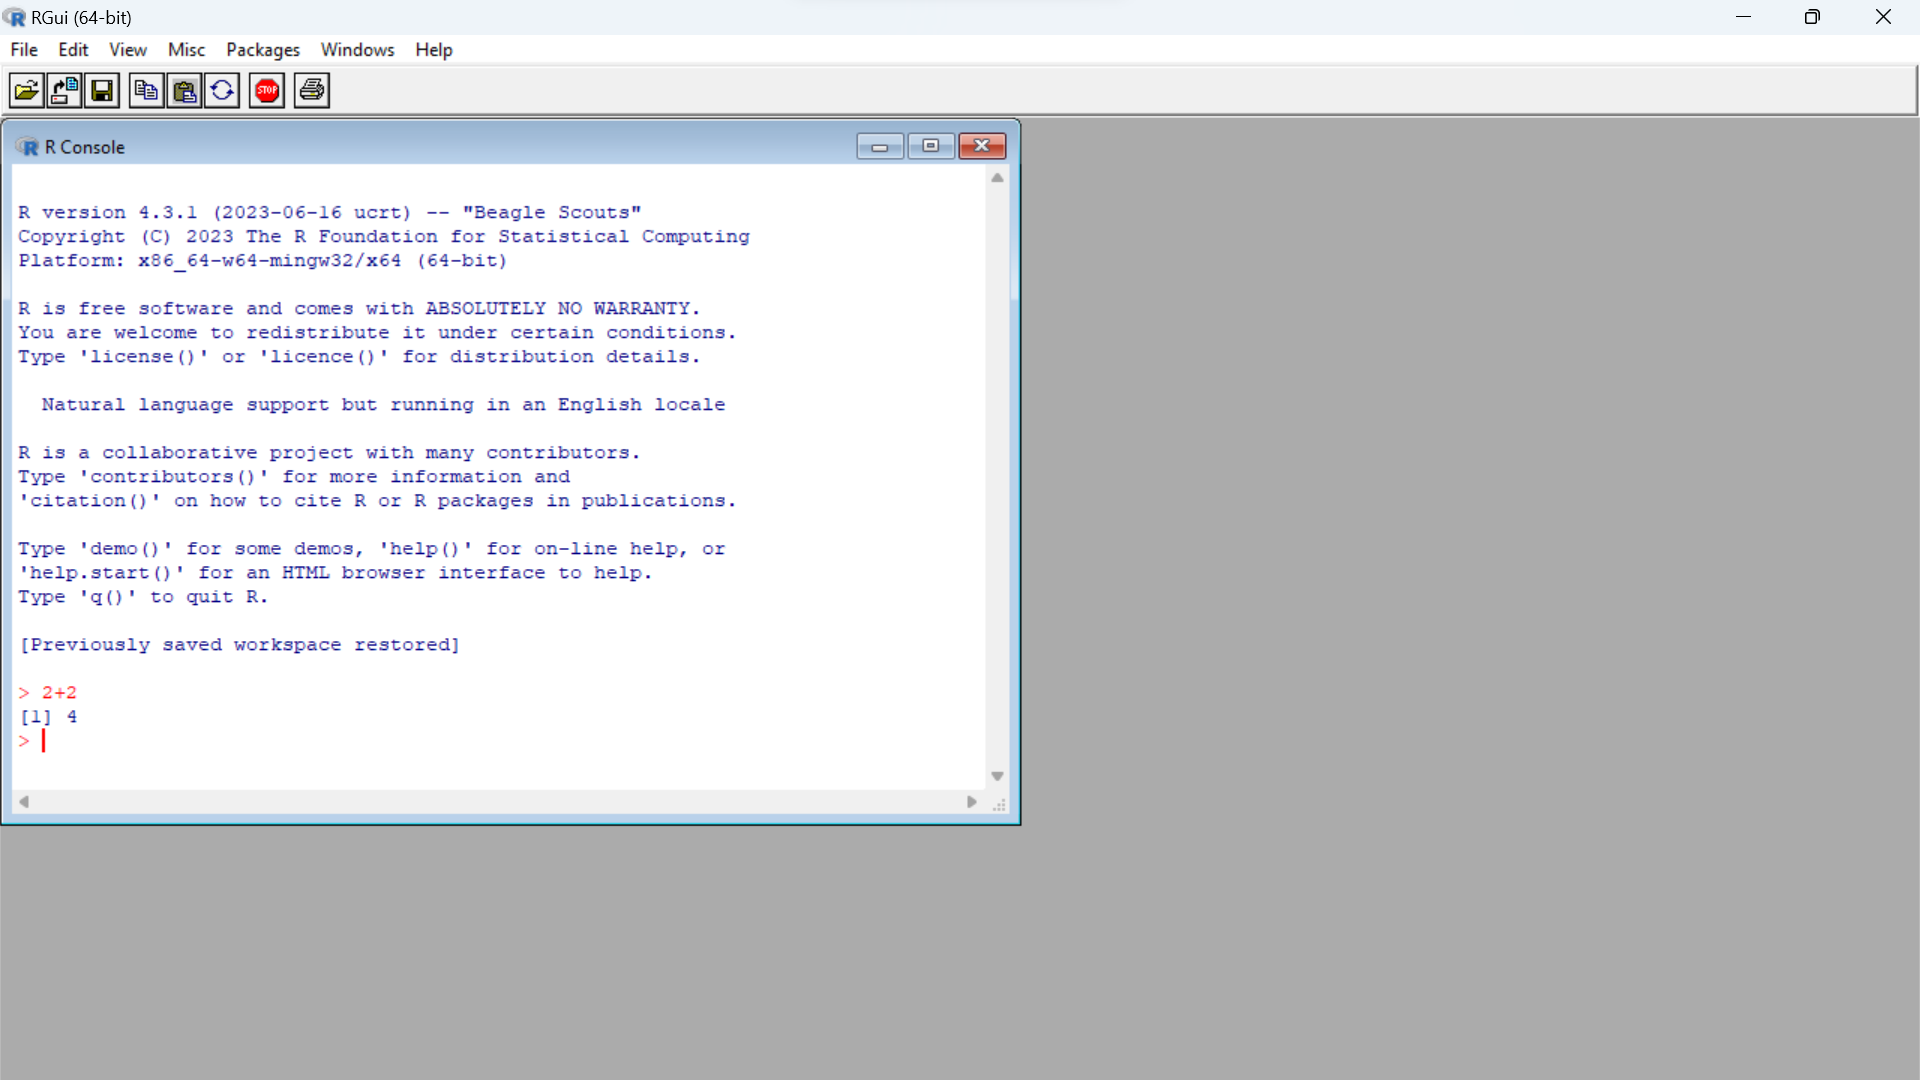
\includegraphics[width=1\linewidth]{./images/Bab1/jendela_r} 

}

\caption{Jendela R.}\label{fig:jendela-R}
\end{figure}

\begin{figure}

{\centering 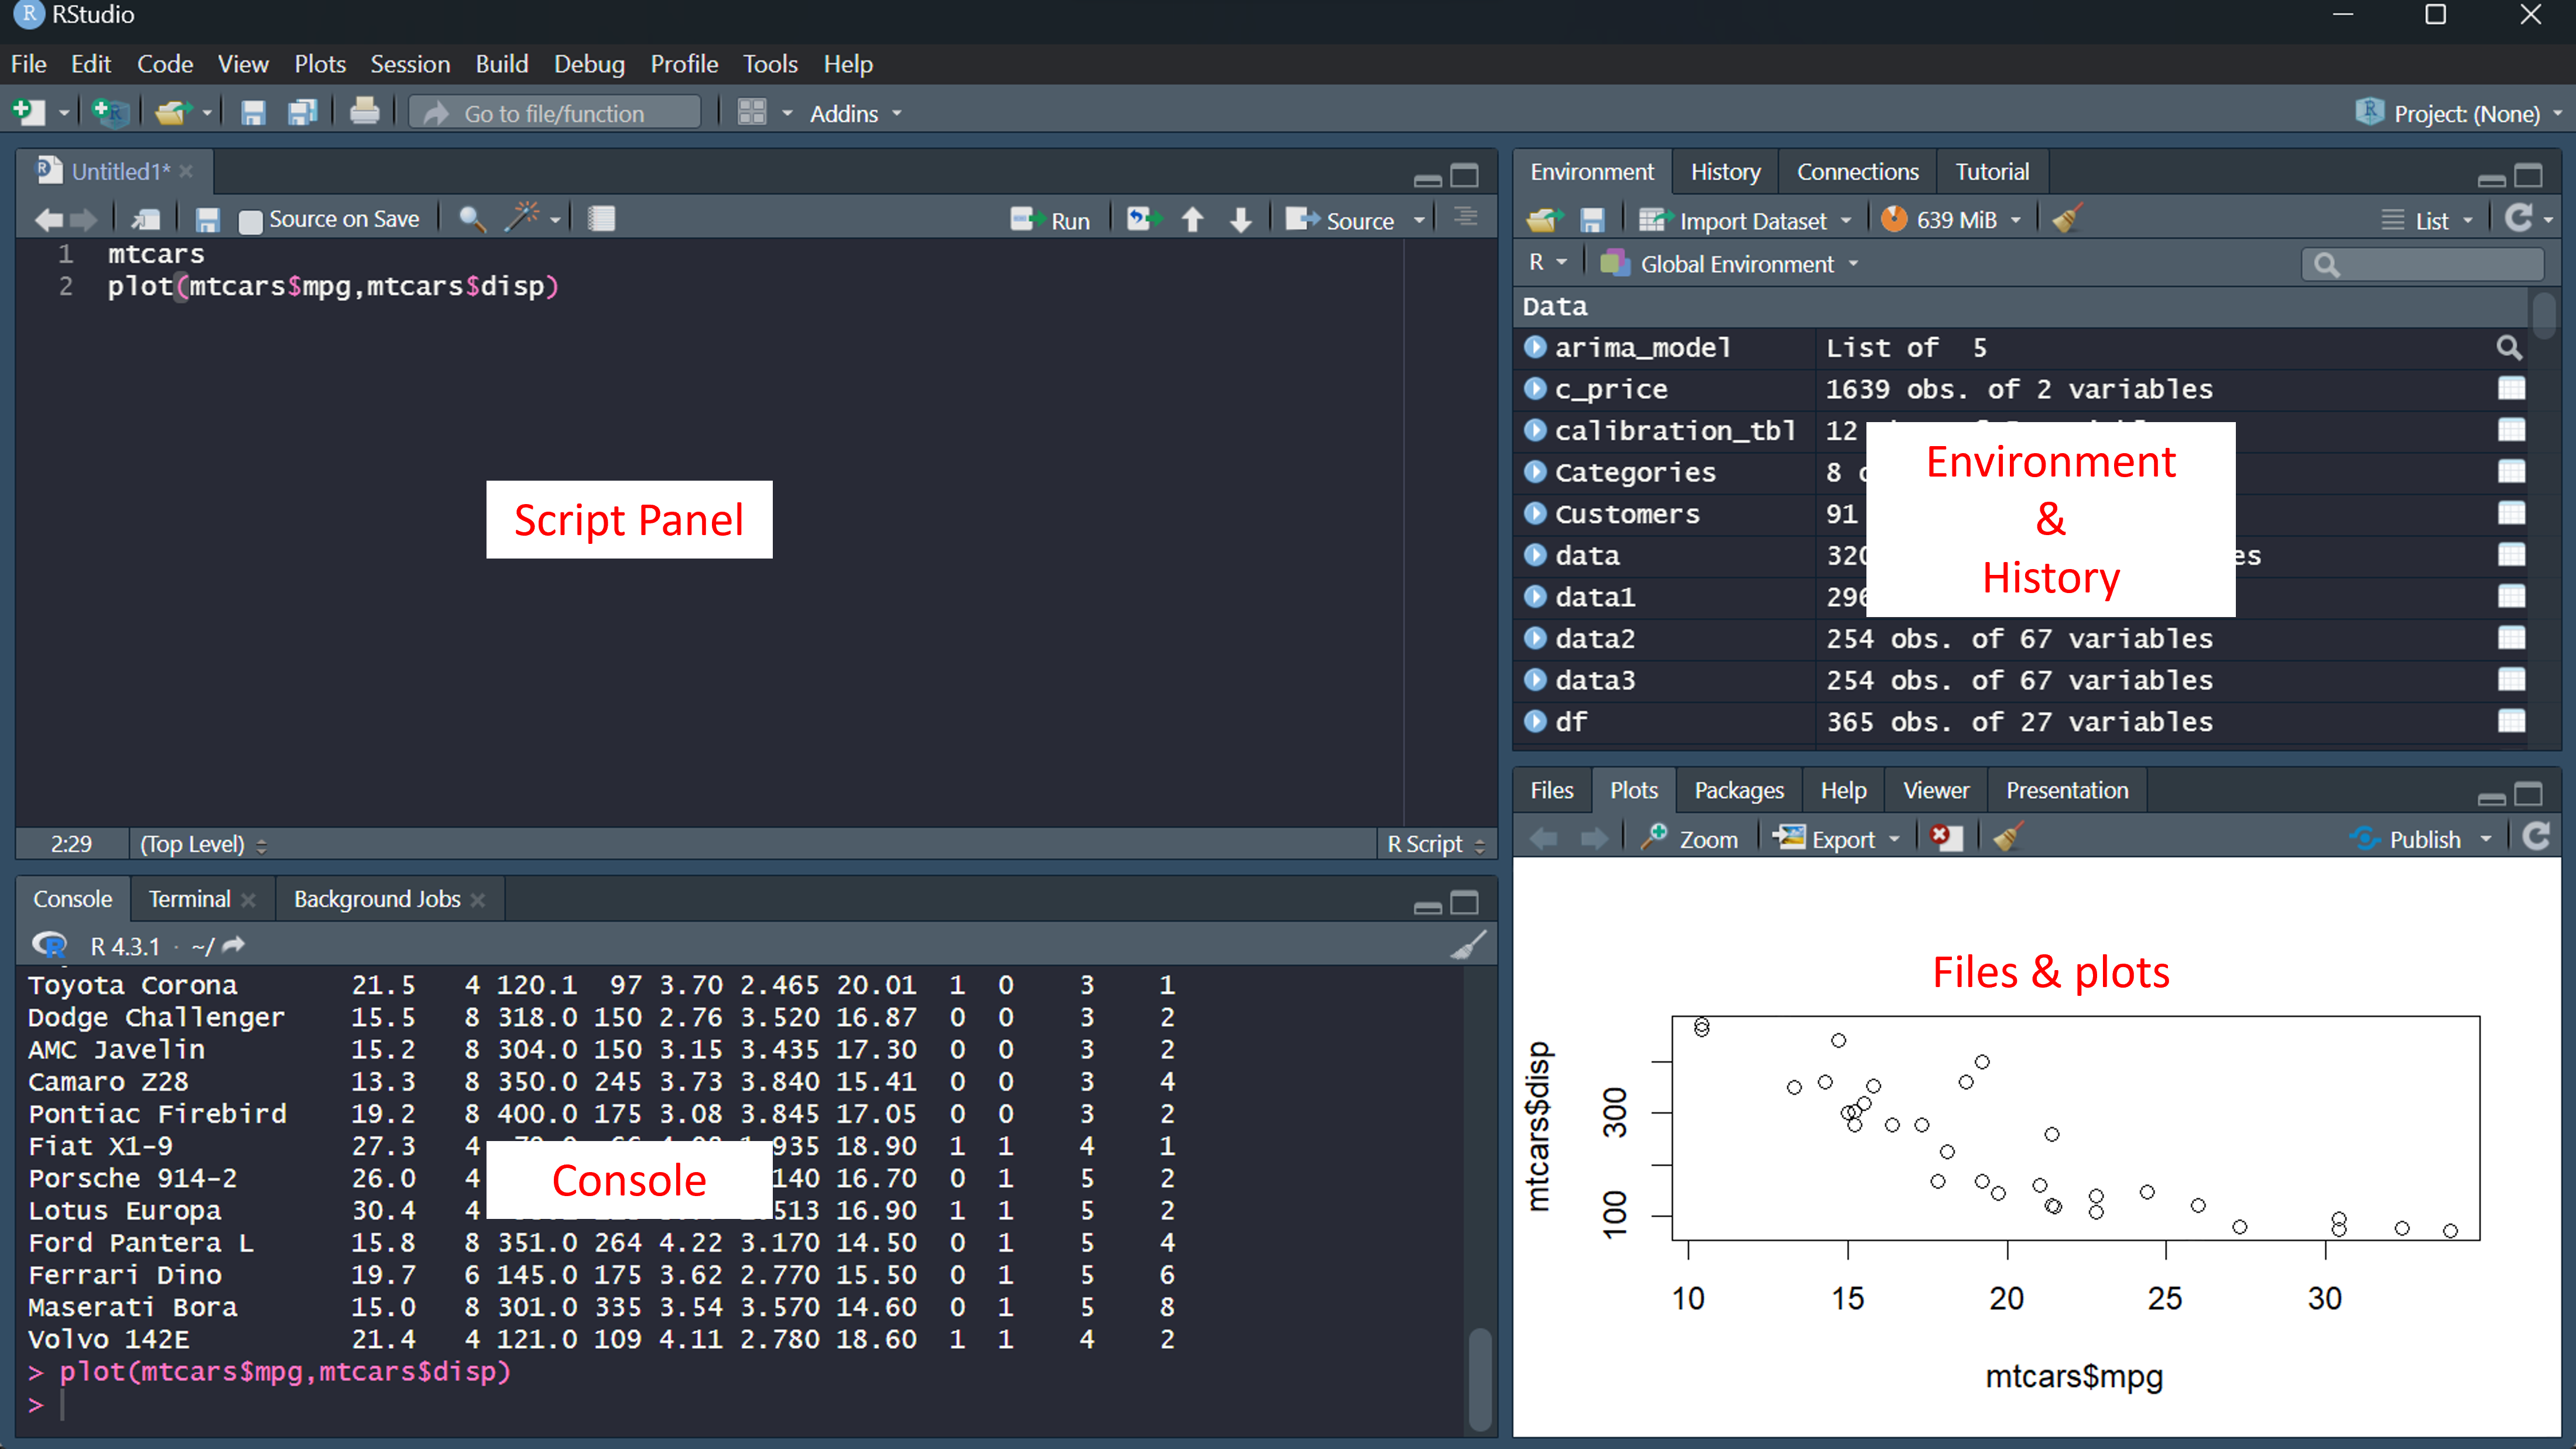
\includegraphics[width=1\linewidth]{./images/Bab1/Rstudio} 

}

\caption{Jendela RStudio.}\label{fig:jendela-RStudio}
\end{figure}

Tampilan ini memiliki beberapa komponen utama, termasuk:

\begin{itemize}
\tightlist
\item
  \textbf{Script Panel:} Tempat Anda menulis kode R dalam skrip.
\item
  \textbf{Console Panel:} Tempat hasil dari kode R ditampilkan, serta tempat Anda dapat menjalankan kode secara interaktif.
\item
  \textbf{Environment Panel:} Menampilkan daftar variabel yang ada dalam sesi R Anda.
\item
  \textbf{History Panel:} Menampilkan riwayat perintah yang telah dijalankan.
\item
  \textbf{Files/Plots/Packages/Help Panel:} Panel tambahan yang membantu Anda mengelola file, visualisasi, pustaka, dan panduan bantuan.
\end{itemize}

Interface ini memudahkan pengguna untuk menulis, menjalankan, dan mengelola kode R serta menganalisis data dengan nyaman.

\hypertarget{sintaks-dasar-r}{%
\section{Sintaks Dasar R}\label{sintaks-dasar-r}}

Berikut ini beberapa kode sederhana yang bisa dipelajari untuk memulai memahami cara kerja Bahasa pemrograman R.

\begin{verbatim}
3+7
3-7
3^7
3/7
3*7
9^(1/3)
\end{verbatim}

\hypertarget{bantuan-help-r}{%
\section{Bantuan (Help) R}\label{bantuan-help-r}}

Salah satu bagian terpenting dalam bekerja dengan bahasa R adalah mengetahui di mana mencari bantuan. R memiliki beberapa fasilitas in-line, selain berbagai sumber daya bantuan di ekosistem R. Anda dapat menggunakan bantuan untuk fungsi tertentu.

\begin{Shaded}
\begin{Highlighting}[]
\FunctionTok{help.start}\NormalTok{()         }\CommentTok{\# menu di mana Anda dapat menavigasi bantuan lokal berbasis web}
\NormalTok{?help                }\CommentTok{\# menu di mana Anda dapat menavigasi bantuan lokal berbasis web }
\NormalTok{?class               }\CommentTok{\# mendapatkan bantuan untuk fungsi \textasciigrave{}class\textasciigrave{}}
\FunctionTok{help}\NormalTok{(class)          }\CommentTok{\# mendapatkan bantuan untuk fungsi \textasciigrave{}class\textasciigrave{}}
\NormalTok{??class              }\CommentTok{\# jika Anda tidak tahu nama fungsi yang Anda cari}
\FunctionTok{help.search}\NormalTok{(}\StringTok{\textquotesingle{}class\textquotesingle{}}\NormalTok{) }\CommentTok{\# jika Anda tidak tahu nama fungsi yang Anda cari}
\end{Highlighting}
\end{Shaded}

\hypertarget{shortcut-penggunaan-rstudio}{%
\section{Shortcut Penggunaan Rstudio}\label{shortcut-penggunaan-rstudio}}

Beberapa petunjuk bermanfaat untuk Rstudio (IDE) meliputi:

\begin{longtable}[]{@{}lcc@{}}
\toprule\noalign{}
Kata Kunci & Perintah & Detail \\
\midrule\noalign{}
\endhead
\bottomrule\noalign{}
\endlastfoot
Ctrl + Return (Enter) & untuk menjalankan baris dari editor & \textasciitilde{} \\
Ctrl + Shift + \# & untuk fokus pada tab bantuan & kontradiktif \\
Alt + Shift + k & untuk jalur pintas keyboard RStudio & \textasciitilde{} \\
Ctrl + r & untuk menelusuri sejarah perintah & \textasciitilde{} \\
Alt + Shift + j & untuk menavigasi antar bagian kode & \textasciitilde{} \\
Ctrl + 1 & untuk melompat ke editor & tab untuk penyelesaian otomatis \\
Ctrl + 2 & untuk melompat ke konsol & tab untuk penyelesaian otomatis \\
Ctrl + 8 & untuk melompat ke environment list & tab untuk pelengkapan otomatis \\
Alt + l & Collapse chunk & Code Folding \\
Alt + Shift + l & Unfold chunk & Code Folding \\
Alt + o & Collapse all & Code Folding \\
Alt + Shift + o & Unfold all & Code Folding \\
Alt + ``-'' & untuk operator penugasan \textless- & \textasciitilde{} \\
Alt + Shift + c & kode komentar/tanda komentar dalam file & .R kontradiktif \\
\end{longtable}

\hypertarget{praktikum}{%
\section{Praktikum}\label{praktikum}}

Buatlah tutorial Instalasi R dan R Studio dalam M.word! Lengkapi setiap prosesnya dengan gambar dan penjelasan.

\hypertarget{operasi-dasar-r}{%
\chapter{Operasi Dasar R}\label{operasi-dasar-r}}

Pemrograman R merujuk pada proses menulis kode dan mengembangkan program menggunakan bahasa pemrograman R. R adalah bahasa pemrograman yang fokus pada analisis statistik, manipulasi data, dan visualisasi. Pada bab ini akan dibahas beberapa unsur utama dalam pemrograman menggunakan bahasa pemrograman R.

\hypertarget{variabel}{%
\section{Variabel}\label{variabel}}

Variabel dalam bahasa pemrograman R digunakan untuk menyimpan dan mengelola data. Variabel memungkinkan Anda untuk menampung nilai-nilai berbagai jenis, seperti angka, karakter (teks), atau nilai logika (benar/salah). Berikut ini adalah cara untuk mendefinisikan dan menggunakan variabel dalam R:

\hypertarget{mendefinisikan-variabel}{%
\subsection{Mendefinisikan Variabel}\label{mendefinisikan-variabel}}

Untuk membuat variabel, Anda cukup menggunakan tanda \textless- atau = untuk memberikan nilai pada variabel.

\begin{Shaded}
\begin{Highlighting}[]
\NormalTok{x }\OtherTok{\textless{}{-}} \DecValTok{10}          \CommentTok{\# Mendefinisikan variabel x }
\NormalTok{y }\OtherTok{=} \DecValTok{12}           \CommentTok{\# Mendefinisikan variabel y}
\end{Highlighting}
\end{Shaded}

\hypertarget{aturan-nama-variabel}{%
\subsection{Aturan Nama Variabel}\label{aturan-nama-variabel}}

\begin{itemize}
\tightlist
\item
  Nama variabel harus dimulai dengan huruf atau tanda \texttt{.}
\item
  Nama variabel bisa terdiri dari huruf, angka, dan tanda \texttt{\_}.
\item
  Karakter khusus seperti +, -, *, /, \^{} dll. tidak diperbolehkan dalam nama variabel.
\item
  Nama variabel bersifat case-sensitive, artinya \texttt{x} dan \texttt{X} dianggap berbeda.
\end{itemize}

\hypertarget{operator}{%
\section{Operator}\label{operator}}

Operator adalah simbol yang mengarahkan compiler untuk melakukan berbagai macam operasi terhadap beberapa penugasan. Operator mensimulasikan berbagai operasi matematis, logika, dan keputusan yang dilakukan pada sekumpulan Bilangan Kompleks, Integer, dan Numerik sebagai penugasan masukan (input). R mendukung sebagian besar empat jenis operator biner antara satu set penugasan. Dalam ini, kita akan melihat berbagai jenis operator yang tersedia di R penggunaannya.

\hypertarget{aritmatika}{%
\subsection{Aritmatika}\label{aritmatika}}

Penggunaan operator aritmatika dalam program R adalah untuk mensimulasikan berbagai operasi matematika, seperti penambahan, pengurangan, perkalian, pembagian, dan modulo. Operator aritmatika yang dilakukan bisa saja berupa nilai skalar, bilangan kompleks, atau vektor.

\begin{longtable}[]{@{}cc@{}}
\toprule\noalign{}
\endhead
\bottomrule\noalign{}
\endlastfoot
\textbf{Operator} & \textbf{R} \\
Penjumlahan & + \\
Pengurangan & - \\
Perkalian & * \\
Divisi/Pembagian & / \\
Pemangkatan & \^{} \\
Modulo & \%\% \\
\end{longtable}

Perhatikan cuplikan R berikut:

\begin{Shaded}
\begin{Highlighting}[]
\NormalTok{x }\OtherTok{\textless{}{-}} \FunctionTok{c}\NormalTok{(}\DecValTok{2}\NormalTok{,}\DecValTok{3}\NormalTok{,}\DecValTok{5}\NormalTok{)    }\CommentTok{\# memuat vektor x}
\NormalTok{y }\OtherTok{\textless{}{-}} \FunctionTok{c}\NormalTok{(}\DecValTok{2}\NormalTok{,}\DecValTok{4}\NormalTok{,}\DecValTok{6}\NormalTok{)    }\CommentTok{\# memuat vektor y}
\NormalTok{x}\SpecialCharTok{+}\NormalTok{y              }\CommentTok{\# hasil penjumahan vektor x dan y}
\FunctionTok{print}\NormalTok{ (x}\SpecialCharTok{+}\NormalTok{y)      }\CommentTok{\# hasil penjumahan vektor x dan y}
\FunctionTok{print}\NormalTok{ (x}\SpecialCharTok{{-}}\NormalTok{y)      }\CommentTok{\# hasil pengurangan vektor x dan y}
\FunctionTok{print}\NormalTok{ (x}\SpecialCharTok{*}\NormalTok{y)      }\CommentTok{\# hasil perkalian vektor x dan y}
\FunctionTok{print}\NormalTok{ (x}\SpecialCharTok{/}\NormalTok{y)      }\CommentTok{\# hasil pembagian vektor x dan y}
\FunctionTok{print}\NormalTok{ (x}\SpecialCharTok{\^{}}\NormalTok{y)      }\CommentTok{\# hasil pemangkatan vektor x dan y}
\FunctionTok{print}\NormalTok{ (x}\SpecialCharTok{\%\%}\NormalTok{y)     }\CommentTok{\# hasil modulo vektor x dan y}
\end{Highlighting}
\end{Shaded}

Adakalanya anda perlu menampilkan keterangan/komentar yang juga melekat pada hasil perhitungan R itu sendiri. Maka anda dapat melakukannya dengan cara berikut:

\begin{Shaded}
\begin{Highlighting}[]
\FunctionTok{cat}\NormalTok{(}\StringTok{"Penjumahan vektor x dan y :"}\NormalTok{, x }\SpecialCharTok{+}\NormalTok{ y, }\StringTok{"}\SpecialCharTok{\textbackslash{}n}\StringTok{"}\NormalTok{)}
\FunctionTok{cat}\NormalTok{(}\StringTok{"Pengurangan vektor x dan y :"}\NormalTok{, x }\SpecialCharTok{{-}}\NormalTok{ y, }\StringTok{"}\SpecialCharTok{\textbackslash{}n}\StringTok{"}\NormalTok{)}
\FunctionTok{cat}\NormalTok{(}\StringTok{"Perkalian vektor x dan y :"}\NormalTok{, x }\SpecialCharTok{*}\NormalTok{ y, }\StringTok{"}\SpecialCharTok{\textbackslash{}n}\StringTok{"}\NormalTok{)}
\FunctionTok{cat}\NormalTok{(}\StringTok{"Pembagian vektor x dan y :"}\NormalTok{, x }\SpecialCharTok{/}\NormalTok{ y, }\StringTok{"}\SpecialCharTok{\textbackslash{}n}\StringTok{"}\NormalTok{)}
\FunctionTok{cat}\NormalTok{ (}\StringTok{"Pemangkatan vektor x dan y :"}\NormalTok{, x }\SpecialCharTok{\^{}}\NormalTok{ y) }
\FunctionTok{cat}\NormalTok{(}\StringTok{"Modulo vektor x dan y :"}\NormalTok{, x }\SpecialCharTok{\%\%}\NormalTok{ y, }\StringTok{"}\SpecialCharTok{\textbackslash{}n}\StringTok{"}\NormalTok{)}
\end{Highlighting}
\end{Shaded}

\textbf{Catatan:} Penjelasan lebih lekap mengenai modulo dapat lihat pada \href{https://www.omnicalculator.com/math/modulo}{link ini}

\hypertarget{relasional}{%
\subsection{Relasional}\label{relasional}}

Operator relasional melakukan operasi perbandingan antara elemen yang bersesuaian pada setiap operan. Mengembalikan nilai Boolean TRUE jika operan pertama memenuhi relasi dibandingkan dengan operan kedua. Nilai TRUE selalu dianggap lebih besar dari FALSE.

\begin{longtable}[]{@{}
  >{\centering\arraybackslash}p{(\columnwidth - 4\tabcolsep) * \real{0.3077}}
  >{\centering\arraybackslash}p{(\columnwidth - 4\tabcolsep) * \real{0.3077}}
  >{\centering\arraybackslash}p{(\columnwidth - 4\tabcolsep) * \real{0.3846}}@{}}
\toprule\noalign{}
\endhead
\bottomrule\noalign{}
\endlastfoot
\textbf{Operator} & \textbf{R} & \textbf{Keterangan} \\
Kurang dari & \textless{} & Mengembalikan TRUE jika elemen yang bersesuaian pada operan pertama lebih kecil dari operan kedua. Selain itu akan mengembalikan FALSE \\
Kurang dari sama dengan & \textless= & Mengembalikan TRUE jika elemen yang bersesuaian pada operan pertama kurang dari atau sama dengan elemen operan kedua. Selain itu akan mengembalikan FALSE \\
Lebih besar dari & \textgreater{} & Mengembalikan TRUE jika elemen yang bersesuaian pada operan pertama lebih besar dari operan kedua. Selain itu akan mengembalikan FALSE \\
Lebih besar dari sama dengan & \textgreater= & Mengembalikan BENAR jika elemen yang bersesuaian pada operan pertama lebih besar atau sama dengan dari operan kedua. Selain itu akan mengembalikan FALSE \\
Sama Dengan & == & Mengembalikan BENAR jika dan hanya jika kedua sisi bernilai sama \\
Tidak Sama dengan & != & Mengembalikan BENAR jika elemen yang bersesuaian pada operan pertama tidak sama dengan dari operan kedua \\
\end{longtable}

\begin{Shaded}
\begin{Highlighting}[]
\NormalTok{x }\OtherTok{\textless{}{-}} \FunctionTok{c}\NormalTok{(}\DecValTok{2}\NormalTok{,}\DecValTok{3}\NormalTok{,}\DecValTok{5}\NormalTok{)    }\CommentTok{\# memuat vektor x}
\NormalTok{y }\OtherTok{\textless{}{-}} \FunctionTok{c}\NormalTok{(}\DecValTok{2}\NormalTok{,}\DecValTok{4}\NormalTok{,}\DecValTok{6}\NormalTok{)    }\CommentTok{\# memuat vektor y}
\FunctionTok{cat}\NormalTok{(}\StringTok{"Vektor x  kurang dari Vektor y:"}\NormalTok{, x }\SpecialCharTok{\textless{}}\NormalTok{ y, }\StringTok{"}\SpecialCharTok{\textbackslash{}n}\StringTok{"}\NormalTok{)}
\FunctionTok{cat}\NormalTok{(}\StringTok{"Vector x kurang dari sama dengan Vector y:"}\NormalTok{, x }\SpecialCharTok{\textless{}=}\NormalTok{ y, }\StringTok{"}\SpecialCharTok{\textbackslash{}n}\StringTok{"}\NormalTok{)}
\FunctionTok{cat}\NormalTok{(}\StringTok{"Vector x lebih besar dari Vector y :"}\NormalTok{, x }\SpecialCharTok{\textgreater{}}\NormalTok{ y, }\StringTok{"}\SpecialCharTok{\textbackslash{}n}\StringTok{"}\NormalTok{)}
\FunctionTok{cat}\NormalTok{(}\StringTok{"Vector x lebih besar dari sama dengan Vector y :"}\NormalTok{, x }\SpecialCharTok{\textgreater{}=}\NormalTok{ y, }\StringTok{"}\SpecialCharTok{\textbackslash{}n}\StringTok{"}\NormalTok{)}
\FunctionTok{cat}\NormalTok{(}\StringTok{"Vector x sama dengan Vector y:"}\NormalTok{, x }\SpecialCharTok{==}\NormalTok{ y,}\StringTok{"}\SpecialCharTok{\textbackslash{}n}\StringTok{"}\NormalTok{) }
\FunctionTok{cat}\NormalTok{(}\StringTok{"Vector x tidak sama dengan Vector y:"}\NormalTok{, x }\SpecialCharTok{!=}\NormalTok{ y) }
\end{Highlighting}
\end{Shaded}

\hypertarget{logika}{%
\subsection{Logika}\label{logika}}

Operator logis mensimulasikan operasi keputusan, berdasarkan operator yang ditentukan antara operan, yang kemudian dievaluasi ke nilai Boolean Benar atau Salah. Nilai bilangan bulat bukan nol dianggap sebagai nilai BENAR, baik itu bilangan kompleks atau bilangan real.

\begin{longtable}[]{@{}
  >{\centering\arraybackslash}p{(\columnwidth - 4\tabcolsep) * \real{0.3077}}
  >{\centering\arraybackslash}p{(\columnwidth - 4\tabcolsep) * \real{0.3077}}
  >{\centering\arraybackslash}p{(\columnwidth - 4\tabcolsep) * \real{0.3846}}@{}}
\toprule\noalign{}
\endhead
\bottomrule\noalign{}
\endlastfoot
\textbf{Operator} & \textbf{R} & \textbf{Keterangan} \\
NOT & ! & Operasi negasi/kebalikan pada status elemen operan \\
AND & \& & Mengembalikan TRUE jika kedua operan bernilai Benar \\
OR & \(|\) & Mengembalikan TRUE jika salah satu operan adalah Benar \\
XOR & \^{} & Mengembalikan TRUE jika salah satu dari kedua elemen pertama operan bernilai Benar \\
\end{longtable}

\begin{Shaded}
\begin{Highlighting}[]
\NormalTok{x }\OtherTok{\textless{}{-}} \FunctionTok{c}\NormalTok{(}\DecValTok{0}\NormalTok{,}\ConstantTok{TRUE}\NormalTok{,}\ConstantTok{FALSE}\NormalTok{)}
\NormalTok{y }\OtherTok{\textless{}{-}} \FunctionTok{c}\NormalTok{(}\ConstantTok{TRUE}\NormalTok{,}\FloatTok{0.1}\NormalTok{,}\DecValTok{4}\SpecialCharTok{+}\NormalTok{3i)}
 
\CommentTok{\# Melakukan operasi logika pada Operan}
\FunctionTok{cat}\NormalTok{(}\StringTok{"Logika Negasi (\textasciitilde{}) untuk vektor x:"}\NormalTok{, }\SpecialCharTok{!}\NormalTok{x, }\StringTok{"}\SpecialCharTok{\textbackslash{}n}\StringTok{"}\NormalTok{) }
\FunctionTok{cat}\NormalTok{(}\StringTok{"Logika Negasi (\textasciitilde{}) untuk vektor y :"}\NormalTok{, }\SpecialCharTok{!}\NormalTok{y, }\StringTok{"}\SpecialCharTok{\textbackslash{}n}\StringTok{"}\NormalTok{) }
\FunctionTok{cat}\NormalTok{ (}\StringTok{"Logika Konjungsi (Dan) :"}\NormalTok{, x }\SpecialCharTok{\&}\NormalTok{ y, }\StringTok{"}\SpecialCharTok{\textbackslash{}n}\StringTok{"}\NormalTok{)}
\FunctionTok{cat}\NormalTok{ (}\StringTok{"Logika Disjungsi (Atau) :"}\NormalTok{, x }\SpecialCharTok{|}\NormalTok{ y, }\StringTok{"}\SpecialCharTok{\textbackslash{}n}\StringTok{"}\NormalTok{)}
\end{Highlighting}
\end{Shaded}

\hypertarget{operator-lain-lain}{%
\subsection{Operator Lain-lain}\label{operator-lain-lain}}

Berikut ini juga ada beberapa operator yang kemungkinan besar juga akan anda perlukan pada saat akan menggunakan R.

\begin{Shaded}
\begin{Highlighting}[]
\NormalTok{x }\OtherTok{\textless{}{-}} \FunctionTok{c}\NormalTok{(}\DecValTok{2}\NormalTok{,}\DecValTok{3}\NormalTok{,}\DecValTok{5}\NormalTok{)                    }\CommentTok{\# memuat vektor x}
\NormalTok{y }\OtherTok{\textless{}{-}} \FunctionTok{c}\NormalTok{(}\DecValTok{2}\NormalTok{,}\DecValTok{4}\NormalTok{,}\DecValTok{6}\NormalTok{)                    }\CommentTok{\# memuat vektor y}
\FunctionTok{sqrt}\NormalTok{(x}\SpecialCharTok{*}\NormalTok{y)                        }\CommentTok{\# Bentuk akar}
\FunctionTok{log}\NormalTok{(x)                           }\CommentTok{\# logaritma }
\FunctionTok{exp}\NormalTok{(y)                           }\CommentTok{\# eksponen}
\NormalTok{(x}\SpecialCharTok{/}\NormalTok{y) }\SpecialCharTok{+}\NormalTok{ y                        }\CommentTok{\# Tanda kurung}
\end{Highlighting}
\end{Shaded}

\textbf{Catatan:} \href{https://www.advernesia.com/blog/matematika/sifat-komutatif-asosiatif-dan-distributif/}{Sifat Komutatif Asosiatif dan Distributif} juga berlaku dalam program R.

\hypertarget{tipe-data}{%
\section{Tipe Data}\label{tipe-data}}

Dalam pemrograman seperti R dan Python, tipe data merupakan konsep penting. Keduanya dapat menggunakan variabel untuk menyimpan tipe yang berbeda-beda, berikut adalah tipe data paling mendasar yang harus diketahui:

\begin{longtable}[]{@{}
  >{\centering\arraybackslash}p{(\columnwidth - 4\tabcolsep) * \real{0.4390}}
  >{\centering\arraybackslash}p{(\columnwidth - 4\tabcolsep) * \real{0.2195}}
  >{\centering\arraybackslash}p{(\columnwidth - 4\tabcolsep) * \real{0.3415}}@{}}
\toprule\noalign{}
\endhead
\bottomrule\noalign{}
\endlastfoot
\textbf{Tipe Data} & \textbf{R} & \textbf{Penjelasan} \\
Double/Float & 5.6 & Bilangan yang mempunyai koma \\
Integer & 5 & Bilangan bulat 1,2,\ldots,n \\
Bolean/Logical & TRUE/FALSE & Benar bernilai 1 dan Salah bernilai 0 \\
String/Character & `Dsciencelabs' & karakter/kalimat bisa berupa huruf angka, dll (diapit tanda '' atau ') \\
Complex & 1 + 5i & Pasangan angka real dan imajiner \\
\end{longtable}

Berikut ini adalah koding R yang dapat digunakan untuk menetapkan kelima tipe data diatas:

\begin{Shaded}
\begin{Highlighting}[]
\NormalTok{d1 }\OtherTok{=} \FloatTok{5.6}                       \CommentTok{\# Tetapkan nilai desimal }
\NormalTok{d2 }\OtherTok{=} \FunctionTok{as.integer}\NormalTok{(}\DecValTok{5}\NormalTok{)             }\CommentTok{\# tetapkan nilai integer}
\NormalTok{d2 }\OtherTok{=}\NormalTok{ 5L                        }\CommentTok{\# cara lain untuk memuat nilai integer di R}
\NormalTok{d3 }\OtherTok{=} \FunctionTok{c}\NormalTok{(}\ConstantTok{TRUE}\NormalTok{,}\ConstantTok{FALSE}\NormalTok{)             }\CommentTok{\# Bolean/Logical}
\NormalTok{d3 }\OtherTok{=} \FunctionTok{as.logical}\NormalTok{(}\FunctionTok{c}\NormalTok{(}\DecValTok{0}\NormalTok{,}\DecValTok{1}\NormalTok{))        }\CommentTok{\# cara lain untuk memuat Bolean/Logical}
\NormalTok{d4 }\OtherTok{=} \FunctionTok{c}\NormalTok{(}\StringTok{"a"}\NormalTok{,}\StringTok{\textquotesingle{}b\textquotesingle{}}\NormalTok{,}\StringTok{\textquotesingle{}123\textquotesingle{}}\NormalTok{)          }\CommentTok{\# String/Character}
\NormalTok{d5 }\OtherTok{=} \DecValTok{1} \SpecialCharTok{+}\NormalTok{ 5i                    }\CommentTok{\# Complex }
\end{Highlighting}
\end{Shaded}

Untuk memeriksa tipe data dalam R:

\begin{Shaded}
\begin{Highlighting}[]
\FunctionTok{class}\NormalTok{(d1)                      }\CommentTok{\# cetak nama kelas variabel}
\FunctionTok{typeof}\NormalTok{(d1)                     }\CommentTok{\# cetak tipe variabel x}
\end{Highlighting}
\end{Shaded}

\hypertarget{statistika-dasar}{%
\section{Statistika Dasar}\label{statistika-dasar}}

\begin{Shaded}
\begin{Highlighting}[]
\NormalTok{data }\OtherTok{\textless{}{-}} \FunctionTok{c}\NormalTok{(}\DecValTok{85}\NormalTok{, }\DecValTok{90}\NormalTok{, }\DecValTok{78}\NormalTok{, }\DecValTok{92}\NormalTok{, }\DecValTok{88}\NormalTok{)  }\CommentTok{\# Data}
\FunctionTok{sum}\NormalTok{(data)                      }\CommentTok{\# Jumlahan data}
\FunctionTok{length}\NormalTok{(data)                   }\CommentTok{\# Banyaknya data}
\FunctionTok{mean}\NormalTok{ (data)                      }\CommentTok{\# Menghitung rata{-}rata}
\FunctionTok{var}\NormalTok{ (data)                     }\CommentTok{\# Menghitung variansi}
\FunctionTok{sd}\NormalTok{ (data)                        }\CommentTok{\# Simpangan baku}
\FunctionTok{min}\NormalTok{(data)                      }\CommentTok{\# Minimum}
\FunctionTok{max}\NormalTok{(data)                      }\CommentTok{\# Maksimum}
\end{Highlighting}
\end{Shaded}

\hypertarget{contoh-pemrograman-dasar}{%
\section{Contoh Pemrograman Dasar}\label{contoh-pemrograman-dasar}}

Berikut ini dilampirkan contoh kasus dasar pemrograman R.

\hypertarget{menghitung-rata-rata}{%
\subsection{Menghitung Rata-rata}\label{menghitung-rata-rata}}

\begin{Shaded}
\begin{Highlighting}[]
\NormalTok{data }\OtherTok{\textless{}{-}} \FunctionTok{c}\NormalTok{(}\DecValTok{85}\NormalTok{, }\DecValTok{90}\NormalTok{, }\DecValTok{78}\NormalTok{, }\DecValTok{92}\NormalTok{, }\DecValTok{88}\NormalTok{)}
\NormalTok{jumlah\_data }\OtherTok{\textless{}{-}} \FunctionTok{length}\NormalTok{(data)}
\NormalTok{total }\OtherTok{\textless{}{-}} \FunctionTok{sum}\NormalTok{(data)}
\NormalTok{rata\_rata }\OtherTok{\textless{}{-}}\NormalTok{ total }\SpecialCharTok{/}\NormalTok{ jumlah\_data}
\FunctionTok{print}\NormalTok{(}\FunctionTok{paste}\NormalTok{(}\StringTok{"Rata{-}rata:"}\NormalTok{, rata\_rata))}
\end{Highlighting}
\end{Shaded}

\begin{verbatim}
## [1] "Rata-rata: 86.6"
\end{verbatim}

\hypertarget{membandingkan-angka}{%
\subsection{Membandingkan Angka}\label{membandingkan-angka}}

\begin{Shaded}
\begin{Highlighting}[]
\NormalTok{a }\OtherTok{\textless{}{-}} \DecValTok{10}
\NormalTok{b }\OtherTok{\textless{}{-}} \DecValTok{20}

\ControlFlowTok{if}\NormalTok{ (a }\SpecialCharTok{\textless{}}\NormalTok{ b) \{}
  \FunctionTok{print}\NormalTok{(}\StringTok{"a lebih kecil dari b"}\NormalTok{)}
\NormalTok{\} }\ControlFlowTok{else} \ControlFlowTok{if}\NormalTok{ (a }\SpecialCharTok{\textgreater{}}\NormalTok{ b) \{}
  \FunctionTok{print}\NormalTok{(}\StringTok{"a lebih besar dari b"}\NormalTok{)}
\NormalTok{\} }\ControlFlowTok{else}\NormalTok{ \{}
  \FunctionTok{print}\NormalTok{(}\StringTok{"a sama dengan b"}\NormalTok{)}
\NormalTok{\}}
\end{Highlighting}
\end{Shaded}

\begin{verbatim}
## [1] "a lebih kecil dari b"
\end{verbatim}

\hypertarget{membandingkan-karakter}{%
\subsection{Membandingkan Karakter}\label{membandingkan-karakter}}

\begin{Shaded}
\begin{Highlighting}[]
\NormalTok{kata1 }\OtherTok{\textless{}{-}} \StringTok{"Apel"}
\NormalTok{kata2 }\OtherTok{\textless{}{-}} \StringTok{"apel"}

\ControlFlowTok{if}\NormalTok{ (kata1 }\SpecialCharTok{==}\NormalTok{ kata2) \{}
  \FunctionTok{print}\NormalTok{(}\StringTok{"kata1 sama dengan kata2"}\NormalTok{)}
\NormalTok{\} }\ControlFlowTok{else}\NormalTok{ \{}
  \FunctionTok{print}\NormalTok{(}\StringTok{"kata1 berbeda dari kata2"}\NormalTok{)}
\NormalTok{\}}
\end{Highlighting}
\end{Shaded}

\begin{verbatim}
## [1] "kata1 berbeda dari kata2"
\end{verbatim}

\hypertarget{mengecek-kondisi-gabungan}{%
\subsection{Mengecek Kondisi Gabungan}\label{mengecek-kondisi-gabungan}}

\begin{Shaded}
\begin{Highlighting}[]
\NormalTok{umur }\OtherTok{\textless{}{-}} \DecValTok{25}
\NormalTok{pendapatan }\OtherTok{\textless{}{-}} \DecValTok{5000}

\ControlFlowTok{if}\NormalTok{ (umur }\SpecialCharTok{\textgreater{}} \DecValTok{18} \SpecialCharTok{\&\&}\NormalTok{ pendapatan }\SpecialCharTok{\textgreater{}} \DecValTok{4000}\NormalTok{) \{}
  \FunctionTok{print}\NormalTok{(}\StringTok{"Anda memenuhi syarat"}\NormalTok{)}
\NormalTok{\} }\ControlFlowTok{else}\NormalTok{ \{}
  \FunctionTok{print}\NormalTok{(}\StringTok{"Anda tidak memenuhi syarat"}\NormalTok{)}
\NormalTok{\}}
\end{Highlighting}
\end{Shaded}

\begin{verbatim}
## [1] "Anda memenuhi syarat"
\end{verbatim}

\hypertarget{penggunaan-operator-logika}{%
\subsection{Penggunaan Operator Logika}\label{penggunaan-operator-logika}}

\begin{Shaded}
\begin{Highlighting}[]
\NormalTok{x }\OtherTok{\textless{}{-}} \DecValTok{5}
\NormalTok{y }\OtherTok{\textless{}{-}} \DecValTok{10}

\ControlFlowTok{if}\NormalTok{ (x }\SpecialCharTok{\textgreater{}} \DecValTok{0} \SpecialCharTok{||}\NormalTok{ y }\SpecialCharTok{\textgreater{}} \DecValTok{0}\NormalTok{) \{}
  \FunctionTok{print}\NormalTok{(}\StringTok{"Salah satu variabel positif"}\NormalTok{)}
\NormalTok{\} }\ControlFlowTok{else}\NormalTok{ \{}
  \FunctionTok{print}\NormalTok{(}\StringTok{"Kedua variabel non{-}positif"}\NormalTok{)}
\NormalTok{\}}
\end{Highlighting}
\end{Shaded}

\begin{verbatim}
## [1] "Salah satu variabel positif"
\end{verbatim}

\hypertarget{pemeriksaan-kondisi-dengan-ifelse}{%
\subsection{Pemeriksaan Kondisi dengan ifelse()}\label{pemeriksaan-kondisi-dengan-ifelse}}

\begin{Shaded}
\begin{Highlighting}[]
\NormalTok{nilai }\OtherTok{\textless{}{-}} \DecValTok{75}
\NormalTok{keterangan }\OtherTok{\textless{}{-}} \FunctionTok{ifelse}\NormalTok{(nilai }\SpecialCharTok{\textgreater{}=} \DecValTok{70}\NormalTok{, }\StringTok{"Lulus"}\NormalTok{, }\StringTok{"Tidak lulus"}\NormalTok{)}
\FunctionTok{print}\NormalTok{(}\FunctionTok{paste}\NormalTok{(}\StringTok{"Nilai:"}\NormalTok{, nilai, }\StringTok{"{-}{-}\textgreater{} Status:"}\NormalTok{, keterangan))}
\end{Highlighting}
\end{Shaded}

\begin{verbatim}
## [1] "Nilai: 75 --> Status: Lulus"
\end{verbatim}

\hypertarget{latihan}{%
\section{Latihan}\label{latihan}}

Berikut adalah beberapa contoh soal latihan dasar pemrograman dalam bahasa pemrograman R:

\begin{enumerate}
\def\labelenumi{\arabic{enumi}.}
\tightlist
\item
  \textbf{Menghitung Luas Lingkaran:} Buatlah sebuah program R yang menerima input berupa jari-jari lingkaran dan menghitung serta mencetak luas lingkaran.
\item
  \textbf{Konversi Suhu:} Buatlah sebuah program R yang dapat mengonversi suhu dari Celsius ke Fahrenheit. Program harus menerima input suhu dalam Celsius dan menghasilkan output suhu dalam Fahrenheit.
\item
  \textbf{Menghitung Faktorial:} Buatlah sebuah program R yang menghitung faktorial dari sebuah bilangan bulat positif. Program harus menerima input bilangan bulat positif dan menghasilkan output faktorialnya.
\item
  \textbf{Mencari Bilangan Prima:} Buatlah sebuah program R yang menerima input sebuah bilangan bulat dan menghasilkan output apakah bilangan tersebut merupakan bilangan prima atau bukan.
\item
  \textbf{Menghitung Pangkat:} Buatlah sebuah program R yang menerima input bilangan dasar dan eksponen, kemudian menghitung hasil dari bilangan dasar dipangkatkan dengan eksponen tersebut.
\item
  \textbf{Menghitung Total Nilai:} Buatlah sebuah program R yang menerima input sejumlah nilai mata kuliah dan menghitung total nilai serta rata-ratanya. Program harus menerima input nilai-nilai mata kuliah dan menghasilkan total nilai serta rata-ratanya.
\item
  \textbf{Menentukan Ganjil/Genap:} Buatlah sebuah program R yang menerima input bilangan bulat dan mencetak apakah bilangan tersebut ganjil atau genap.
\item
  \textbf{Menghitung Keliling dan Luas Persegi:} Buatlah sebuah program R yang menerima input panjang sisi persegi dan menghitung serta mencetak keliling dan luasnya.
\end{enumerate}

\hypertarget{struktur-data}{%
\chapter{Struktur Data}\label{struktur-data}}

Struktur data dalam R adalah cara di mana Anda dapat mengatur dan menyimpan data dalam bentuk yang terstruktur agar mudah diakses, dikelola, dan dimanipulasi. Struktur data memungkinkan Anda untuk mengelompokkan nilai-nilai data ke dalam objek yang sesuai dengan jenis dan sifat data yang Anda miliki. R memiliki beberapa jenis struktur data yang dapat digunakan untuk berbagai tujuan.

\begin{figure}

{\centering 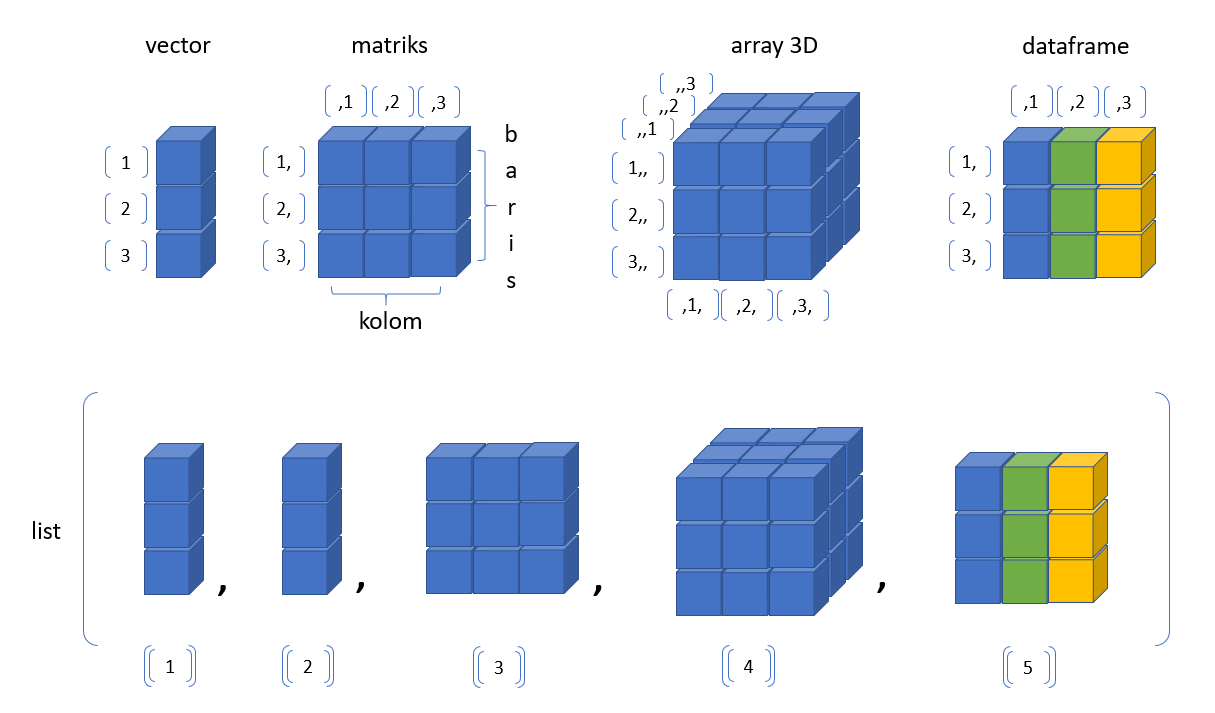
\includegraphics[width=1\linewidth]{./images/Bab3/Struktur_Data} 

}

\caption{Struktur Data dalam R}\label{fig:struktur-data}
\end{figure}

\hypertarget{vektor}{%
\section{Vektor}\label{vektor}}

Elemen paling dasar dalam R adalah vektor, yang berisikan kumpulan elemen data dengan tipe yang sama. Terdapat dua jenis vector, yaitu vector numerik dan vector karakter. Misalnya:

\begin{Shaded}
\begin{Highlighting}[]
\NormalTok{vektor }\OtherTok{\textless{}{-}} \FunctionTok{seq}\NormalTok{(}\AttributeTok{from=}\DecValTok{10}\NormalTok{, }\AttributeTok{to=}\DecValTok{21}\NormalTok{, }\AttributeTok{by=}\DecValTok{1}\NormalTok{)      }\CommentTok{\# fungsi \textasciigrave{}seq()\textasciigrave{} dengan "by"}
\NormalTok{vektor}\OtherTok{\textless{}{-}} \FunctionTok{seq}\NormalTok{(}\AttributeTok{from=}\DecValTok{10}\NormalTok{, }\AttributeTok{to=}\DecValTok{21}\NormalTok{, }\AttributeTok{len=}\DecValTok{12}\NormalTok{)     }\CommentTok{\# fungsi \textasciigrave{}seq()\textasciigrave{} dengan "len"}
\NormalTok{vektor }\OtherTok{\textless{}{-}} \DecValTok{10}\SpecialCharTok{:}\DecValTok{21}                          \CommentTok{\# tetapkan data dalam vektor }
\NormalTok{vektor }\OtherTok{\textless{}{-}}\NormalTok{ vektor}\SpecialCharTok{+}\DecValTok{2}                       \CommentTok{\# Operasi berdasarkan elemen}
\NormalTok{vektor }\OtherTok{\textless{}{-}}\NormalTok{ vektor}\SpecialCharTok{*}\DecValTok{2}                       \CommentTok{\# Tambahkan 2 untuk setiap elemen }
\NormalTok{vektor }\OtherTok{\textless{}{-}}\NormalTok{ vektor}\SpecialCharTok{\^{}}\DecValTok{2}                       \CommentTok{\# Pangkat 2 untuk setiap elemen }
\NormalTok{vektor }\OtherTok{\textless{}{-}} \FunctionTok{sqrt}\NormalTok{(vektor)                   }\CommentTok{\# Akar kuadrat untuk setiap elemen}
\NormalTok{vektor }\OtherTok{\textless{}{-}} \FunctionTok{log}\NormalTok{(vektor)                    }\CommentTok{\# Logaritma untuk setiap elemen}
\NormalTok{vektor}\OtherTok{\textless{}{-}} \FunctionTok{c}\NormalTok{(}\FloatTok{0.5}\NormalTok{, }\FloatTok{0.6}\NormalTok{)                     }\CommentTok{\# Numerik}
\NormalTok{vektor }\OtherTok{\textless{}{-}} \FunctionTok{c}\NormalTok{(}\ConstantTok{TRUE}\NormalTok{, }\ConstantTok{FALSE}\NormalTok{)                 }\CommentTok{\# Logis}
\NormalTok{vektor }\OtherTok{\textless{}{-}} \FunctionTok{c}\NormalTok{(T, F)                        }\CommentTok{\# Logis}
\NormalTok{vektor }\OtherTok{\textless{}{-}} \FunctionTok{c}\NormalTok{(}\StringTok{"a"}\NormalTok{, }\StringTok{"b"}\NormalTok{, }\StringTok{"c"}\NormalTok{)               }\CommentTok{\# Karakter}
\NormalTok{vektor }\OtherTok{\textless{}{-}} \DecValTok{9}\SpecialCharTok{:}\DecValTok{29}                           \CommentTok{\# Integer}
\NormalTok{vektor }\OtherTok{\textless{}{-}} \FunctionTok{c}\NormalTok{(}\DecValTok{1}\SpecialCharTok{+}\NormalTok{0i, }\DecValTok{2}\SpecialCharTok{+}\NormalTok{4i)                  }\CommentTok{\# Kompleks}
\NormalTok{vektor }\OtherTok{\textless{}{-}} \FunctionTok{vector}\NormalTok{(}\StringTok{"numeric"}\NormalTok{, }\AttributeTok{length =} \DecValTok{10}\NormalTok{) }\CommentTok{\# untuk inisialisasi vektor.}
\end{Highlighting}
\end{Shaded}

\textbf{Catatan:} Menurut \href{https://stat.ethz.ch/R-manual/R-devel/doc/manual/R-lang.html\#Objects}{dokumentasi R} untuk \texttt{typeof()} dan \texttt{class()}, pernyataan tentang ``perbedaan utama/main difference'' adalah tidak benar. Kelas adalah atribut dari objek yang dapat ditetapkan terlepas dari mode penyimpanan internalnya, sedangkan \texttt{typeof()} menentukan tipe (R internal) atau mode penyimpanan dari objek apa pun. Salah satu menggambarkan karakteristik logis sedangkan yang lain adalah karakteristik fisik dari suatu objek.

\begin{Shaded}
\begin{Highlighting}[]
\FunctionTok{class}\NormalTok{(vektor)                            }\CommentTok{\# Periksa kelas vektor}
\FunctionTok{as.numeric}\NormalTok{(vektor)                       }\CommentTok{\# Menetapkan vektor sebagai numerik}
\FunctionTok{as.logical}\NormalTok{(vektor)                       }\CommentTok{\# Menetapkan vektor sebagai logis}
\FunctionTok{as.character}\NormalTok{(vektor)                     }\CommentTok{\# Menetapkan vektor sebagai karakter}
\FunctionTok{as.numeric}\NormalTok{(}\FunctionTok{c}\NormalTok{(}\ConstantTok{FALSE}\NormalTok{,}\ConstantTok{TRUE}\NormalTok{,}\ConstantTok{TRUE}\NormalTok{,}\ConstantTok{FALSE}\NormalTok{))     }\CommentTok{\# Menetapkan vektor logis sebagai angka }
\end{Highlighting}
\end{Shaded}

Terkadang, R tidak dapat menemukan cara untuk memaksa suatu objek dan ini dapat menghasilkan NA.

\begin{Shaded}
\begin{Highlighting}[]
\NormalTok{vektor }\OtherTok{\textless{}{-}} \FunctionTok{c}\NormalTok{(}\StringTok{"a"}\NormalTok{, }\StringTok{"b"}\NormalTok{, }\StringTok{"c"}\NormalTok{,}\StringTok{"1"}\NormalTok{)             }\CommentTok{\# menetapkan nilai vektor}
\FunctionTok{as.numeric}\NormalTok{(vektor)                       }\CommentTok{\# menetapkan vektor sebagai numerik}
\end{Highlighting}
\end{Shaded}

\begin{verbatim}
## Warning: NAs introduced by coercion
\end{verbatim}

\begin{Shaded}
\begin{Highlighting}[]
\FunctionTok{as.logical}\NormalTok{(vektor)                       }\CommentTok{\# menetapkan vektor sebagai logis}
\FunctionTok{as.complex}\NormalTok{(vektor)                       }\CommentTok{\# menetapkan vektor sebagai karakter}
\end{Highlighting}
\end{Shaded}

\begin{verbatim}
## Warning: NAs introduced by coercion
\end{verbatim}

\textbf{Catatan:} Saat paksaan tidak masuk akal terjadi, Anda biasanya akan mendapat peringatan dari R.

Kita sudah melihat bahwa elemen dasar dari objek R adalah vektor. Vektor dapat ditetapkan dengan berbagai jenis berikut:

\begin{itemize}
\tightlist
\item
  \textbf{character:} di mana setiap elemen adalah string, mis., urutan simbol alfanumerik.
\item
  \textbf{numeric:} di mana setiap elemen adalah \href{https://en.wikipedia.org/wiki/Real_number}{bilangan real} dalam format floating point \href{https://en.wikipedia.org/wiki/Double-precision_floating-point_format}{presisi ganda}.
\item
  \textbf{integer:} di mana setiap elemen adalah \href{https://en.wikipedia.org/wiki/Integer}{integer}.
\item
  \textbf{logis:} di mana setiap elemen adalah TRUE, FALSE, atau NA3
\item
  \textbf{complex:} di mana setiap elemen adalah bilangan kompleks.
\end{itemize}

\hypertarget{matriks}{%
\section{Matriks}\label{matriks}}

Matriks adalah vektor dengan atribut dimensi. Matriks dibuat berdasarkan kolom, sehingga entri dapat dianggap dimulai dari sudut ``kiri atas'' dan mengalir di kolom.

\begin{Shaded}
\begin{Highlighting}[]
\NormalTok{matriks }\OtherTok{\textless{}{-}} \FunctionTok{matrix}\NormalTok{(}\FunctionTok{c}\NormalTok{(}\DecValTok{1}\NormalTok{, }\DecValTok{2}\NormalTok{, }\DecValTok{3}\NormalTok{, }\DecValTok{4}\NormalTok{, }\DecValTok{5}\NormalTok{, }\DecValTok{6}\NormalTok{), }\AttributeTok{nrow =} \DecValTok{2}\NormalTok{, }\AttributeTok{ncol =} \DecValTok{3}\NormalTok{)}
\NormalTok{matriks}
\end{Highlighting}
\end{Shaded}

\begin{verbatim}
##      [,1] [,2] [,3]
## [1,]    1    3    5
## [2,]    2    4    6
\end{verbatim}

Matriks juga dapat dibuat langsung dari vektor dengan menambahkan atribut dimensi.

\begin{Shaded}
\begin{Highlighting}[]
\NormalTok{matriks }\OtherTok{\textless{}{-}} \DecValTok{1}\SpecialCharTok{:}\DecValTok{6}                         \CommentTok{\# Membuat vektor}
\FunctionTok{dim}\NormalTok{(matriks) }\OtherTok{\textless{}{-}} \FunctionTok{c}\NormalTok{(}\DecValTok{2}\NormalTok{, }\DecValTok{3}\NormalTok{)                }\CommentTok{\# rubah vektor sebagai matriks sebesar 2x3}
\NormalTok{matriks                                }\CommentTok{\# Mencetak hasilnya}
\end{Highlighting}
\end{Shaded}

Matriks dapat dibuat dengan pengikatan kolom atau pengikatan baris dengan fungsi \texttt{cbind()} dan \texttt{rbind()}.

\begin{Shaded}
\begin{Highlighting}[]
\NormalTok{x }\OtherTok{\textless{}{-}} \DecValTok{1}\SpecialCharTok{:}\DecValTok{3}                              \CommentTok{\# Membuat vektor \textasciigrave{}x\textasciigrave{}}
\NormalTok{y }\OtherTok{\textless{}{-}} \DecValTok{10}\SpecialCharTok{:}\DecValTok{12}                            \CommentTok{\# Membuat vektor \textasciigrave{}y\textasciigrave{}}
\FunctionTok{cbind}\NormalTok{(x, y)                           }\CommentTok{\# Menggabungkan vektor \textasciigrave{}x\textasciigrave{} dan\textasciigrave{} y\textasciigrave{} dengan kolom}
\FunctionTok{rbind}\NormalTok{(x, y)                           }\CommentTok{\# Menggabungkan vektor \textasciigrave{}x\textasciigrave{} dan\textasciigrave{} y\textasciigrave{} dengan baris}
\end{Highlighting}
\end{Shaded}

\hypertarget{array}{%
\section{Array}\label{array}}

Array mirip dengan matrix, tetapi dapat memiliki lebih dari dua dimensi. Masing-masing dimensi dalam array memiliki ukuran tertentu.

\begin{Shaded}
\begin{Highlighting}[]
\NormalTok{array\_data }\OtherTok{\textless{}{-}} \FunctionTok{array}\NormalTok{(}\FunctionTok{c}\NormalTok{(}\DecValTok{1}\NormalTok{, }\DecValTok{2}\NormalTok{, }\DecValTok{3}\NormalTok{, }\DecValTok{4}\NormalTok{, }\DecValTok{5}\NormalTok{, }\DecValTok{6}\NormalTok{), }\AttributeTok{dim =} \FunctionTok{c}\NormalTok{(}\DecValTok{2}\NormalTok{, }\DecValTok{3}\NormalTok{, }\DecValTok{1}\NormalTok{))}
\end{Highlighting}
\end{Shaded}

\hypertarget{faktor}{%
\section{Faktor}\label{faktor}}

Faktor-faktor digunakan untuk mewakili data kategorikal dan dapat menjadi tidak teratur atau teratur. Orang dapat menganggap faktor sebagai vektor integer di mana setiap integer memiliki label. Menggunakan faktor dengan label lebih baik daripada menggunakan bilangan bulat karena faktor menggambarkan diri sendiri. Memiliki variabel yang memiliki nilai ``Laki-laki'' dan ``Perempuan'' lebih baik daripada variabel yang memiliki nilai 1 dan 2. Objek-objek dapat dibuat dengan fungsi \texttt{faktor()}.

\begin{Shaded}
\begin{Highlighting}[]
\NormalTok{x }\OtherTok{\textless{}{-}} \FunctionTok{factor}\NormalTok{(}\FunctionTok{c}\NormalTok{(}\StringTok{"yes"}\NormalTok{,}\StringTok{"no"}\NormalTok{,}\StringTok{"yes"}\NormalTok{,}\StringTok{"no"}\NormalTok{))  }\CommentTok{\# Membuat objek faktor}
\NormalTok{x                                      }\CommentTok{\# Cetak hasilnya}
\FunctionTok{table}\NormalTok{(x)                               }\CommentTok{\# Tabel dari \textasciigrave{}x\textasciigrave{}}
\FunctionTok{unclass}\NormalTok{(x)                             }\CommentTok{\# Melihat representasi faktor yang mendasarinya}
\FunctionTok{attr}\NormalTok{(x,}\StringTok{"levels"}\NormalTok{)                       }\CommentTok{\# Melihat representasi faktor yang mendasarinya}
\end{Highlighting}
\end{Shaded}

\hypertarget{data-frame}{%
\section{Data Frame}\label{data-frame}}

Kerangka data (data frame) adalah tabel atau struktur mirip array dua dimensi di mana setiap kolom berisi nilai satu variabel dan setiap baris berisi satu set nilai dari setiap kolom.

Berikut ini adalah karakteristik data frame.

\begin{itemize}
\tightlist
\item
  Nama kolom tidak boleh kosong;
\item
  Nama baris harus unik;
\item
  Data yang disimpan dalam data frame bisa dari numerik, faktor atau tipe karakter;
\item
  Setiap kolom harus berisi jumlah item data yang sama.
\end{itemize}

\begin{Shaded}
\begin{Highlighting}[]
\CommentTok{\# Buat data frame pertama.}
\NormalTok{df1 }\OtherTok{\textless{}{-}} \FunctionTok{data.frame}\NormalTok{(}\AttributeTok{id =} \FunctionTok{c}\NormalTok{ (}\DecValTok{1}\SpecialCharTok{:}\DecValTok{5}\NormalTok{), }
                \AttributeTok{name =} \FunctionTok{c}\NormalTok{(}\StringTok{"Julian"}\NormalTok{,}\StringTok{"Vanessa"}\NormalTok{,}\StringTok{"Jeffry"}\NormalTok{,}\StringTok{"Angel"}\NormalTok{,}\StringTok{"Nikki"}\NormalTok{),}
              \AttributeTok{salary =} \FunctionTok{c}\NormalTok{(}\FloatTok{623.3}\NormalTok{,}\FloatTok{515.2}\NormalTok{,}\FloatTok{611.0}\NormalTok{,}\FloatTok{729.0}\NormalTok{,}\FloatTok{843.25}\NormalTok{), }
          \AttributeTok{start\_date =} \FunctionTok{as.Date}\NormalTok{(}\FunctionTok{c}\NormalTok{(}\StringTok{"2022{-}01{-}01"}\NormalTok{, }\StringTok{"2022{-}09{-}23"}\NormalTok{, }\StringTok{"2022{-}11{-}15"}\NormalTok{,                                               }\StringTok{"2022{-}05{-}11"}\NormalTok{, }\StringTok{"2022{-}03{-}27"}\NormalTok{)),}
                \AttributeTok{dept =} \FunctionTok{c}\NormalTok{(}\StringTok{"DS"}\NormalTok{,}\StringTok{"DS"}\NormalTok{,}\StringTok{"BA"}\NormalTok{,}\StringTok{"DA"}\NormalTok{,}\StringTok{"DS"}\NormalTok{), }\AttributeTok{stringsAsFactors =}\NormalTok{ F)}
\NormalTok{df1}
\end{Highlighting}
\end{Shaded}

\begin{Shaded}
\begin{Highlighting}[]
\CommentTok{\# Buat data frame kedua.}
\NormalTok{df2 }\OtherTok{\textless{}{-}}\FunctionTok{data.frame}\NormalTok{(}\AttributeTok{id =} \FunctionTok{c}\NormalTok{ (}\DecValTok{6}\SpecialCharTok{:}\DecValTok{10}\NormalTok{), }
               \AttributeTok{name =} \FunctionTok{c}\NormalTok{(}\StringTok{"Ardifo"}\NormalTok{,}\StringTok{"Irene"}\NormalTok{,}\StringTok{"Kefas"}\NormalTok{,}\StringTok{"Sherly"}\NormalTok{,}\StringTok{"Bakti"}\NormalTok{),}
             \AttributeTok{salary =} \FunctionTok{c}\NormalTok{(}\FloatTok{578.0}\NormalTok{,}\FloatTok{722.5}\NormalTok{,}\FloatTok{632.8}\NormalTok{,}\FloatTok{632.8}\NormalTok{,}\ConstantTok{NA}\NormalTok{), }
         \AttributeTok{start\_date =} \FunctionTok{as.Date}\NormalTok{(}\FunctionTok{c}\NormalTok{(}\StringTok{"2022{-}05{-}21"}\NormalTok{,}\StringTok{"2022{-}07{-}30"}\NormalTok{,}\StringTok{"2022{-}06{-}17"}\NormalTok{,}
                                \StringTok{"2022{-}07{-}30"}\NormalTok{,}\StringTok{"2018{-}09{-}03"}\NormalTok{)),}
               \AttributeTok{dept =} \FunctionTok{c}\NormalTok{(}\StringTok{"Actuaries"}\NormalTok{,}\StringTok{"Actuaries"}\NormalTok{,}\StringTok{"CA"}\NormalTok{,}\StringTok{"DE"}\NormalTok{,}\StringTok{"Lecturer"}\NormalTok{),}\AttributeTok{stringsAsFactors =}\NormalTok{ F)}
\NormalTok{df2}
\end{Highlighting}
\end{Shaded}

\begin{Shaded}
\begin{Highlighting}[]
\NormalTok{df3 }\OtherTok{\textless{}{-}} \FunctionTok{rbind}\NormalTok{(df1,df2)                  }\CommentTok{\# Gabungkan dua frame data}
\FunctionTok{print}\NormalTok{(df3)                             }\CommentTok{\# Cetak hasilnya \textasciigrave{}df3\textasciigrave{}}
\FunctionTok{head}\NormalTok{(df3)                              }\CommentTok{\# Cetak enam baris pertama}
\FunctionTok{head}\NormalTok{(df3,}\DecValTok{6}\NormalTok{)                            }\CommentTok{\# Cetak enam baris pertama}
\CommentTok{\#View(df3)                             \# Menggunakan RStudio seperti penampil Excel}
\FunctionTok{class}\NormalTok{(df3)                             }\CommentTok{\# objeknya bertipe data.frame}
\FunctionTok{str}\NormalTok{(df3)                               }\CommentTok{\# Dapatkan struktur data frame}
\FunctionTok{dim}\NormalTok{(df3)                               }\CommentTok{\# Periksa dimensi data}
\end{Highlighting}
\end{Shaded}

Data frame biasanya dibuat dengan membaca dalam dataset menggunakan \texttt{read.table()} atau \texttt{read.csv\ ()}. Namun, data frame juga dapat dibuat secara eksplisit dengan fungsi \texttt{data.frame()} atau mereka dapat dipaksakan dari jenis objek lain seperti list.

\hypertarget{lists}{%
\section{Lists}\label{lists}}

List dalam R adalah struktur data yang mengizinkan Anda untuk menyimpan berbagai jenis objek, termasuk vektor, matriks, array, dataframe, dan objek list lainnya, dalam satu objek tunggal. Ini memungkinkan Anda untuk membuat struktur data yang kompleks dan fleksibel dengan menggabungkan objek-objek yang berbeda ke dalam satu wadah. List sering digunakan ketika Anda perlu mengorganisir dan mengelompokkan objek-objek yang terkait.

Berikut adalah contoh penggunaan dan pembuatan list dalam R:

\begin{Shaded}
\begin{Highlighting}[]
\CommentTok{\# Membuat vektor dan matriks}
\NormalTok{vektor }\OtherTok{\textless{}{-}} \FunctionTok{c}\NormalTok{(}\FloatTok{1.5}\NormalTok{, }\FloatTok{2.7}\NormalTok{, }\FloatTok{3.2}\NormalTok{, }\FloatTok{4.0}\NormalTok{)}
\NormalTok{matriks }\OtherTok{\textless{}{-}} \FunctionTok{matrix}\NormalTok{(}\FunctionTok{c}\NormalTok{(}\DecValTok{1}\NormalTok{, }\DecValTok{2}\NormalTok{, }\DecValTok{3}\NormalTok{, }\DecValTok{4}\NormalTok{, }\DecValTok{5}\NormalTok{, }\DecValTok{6}\NormalTok{), }\AttributeTok{nrow =} \DecValTok{2}\NormalTok{, }\AttributeTok{ncol =} \DecValTok{3}\NormalTok{)}
\end{Highlighting}
\end{Shaded}

\begin{Shaded}
\begin{Highlighting}[]
\CommentTok{\# Membuat dataframe}
\NormalTok{data\_frame }\OtherTok{\textless{}{-}} \FunctionTok{data.frame}\NormalTok{(}\AttributeTok{name =} \FunctionTok{c}\NormalTok{(}\StringTok{"Alice"}\NormalTok{, }\StringTok{"Bakti"}\NormalTok{, }\StringTok{"Charlie"}\NormalTok{),}
                         \AttributeTok{age =} \FunctionTok{c}\NormalTok{(}\DecValTok{25}\NormalTok{, }\DecValTok{30}\NormalTok{, }\DecValTok{28}\NormalTok{),}
                         \AttributeTok{score =} \FunctionTok{c}\NormalTok{(}\DecValTok{95}\NormalTok{, }\DecValTok{88}\NormalTok{, }\DecValTok{76}\NormalTok{))}
\end{Highlighting}
\end{Shaded}

\begin{Shaded}
\begin{Highlighting}[]
\NormalTok{faktor }\OtherTok{\textless{}{-}} \StringTok{"List, Sudah Jadi"}
\end{Highlighting}
\end{Shaded}

\begin{Shaded}
\begin{Highlighting}[]
\CommentTok{\# Membuat list}
\NormalTok{my\_list }\OtherTok{\textless{}{-}} \FunctionTok{list}\NormalTok{(vektor, matriks, data\_frame, faktor)}
\end{Highlighting}
\end{Shaded}

\begin{Shaded}
\begin{Highlighting}[]
\CommentTok{\# Menampilkan list}
\FunctionTok{print}\NormalTok{(my\_list)}
\end{Highlighting}
\end{Shaded}

Anda juga dapat memberi nama pada setiap elemen dalam list untuk membuat list yang lebih mudah dibaca:

\begin{Shaded}
\begin{Highlighting}[]
\NormalTok{nama\_list }\OtherTok{\textless{}{-}} \FunctionTok{list}\NormalTok{(}\AttributeTok{elemen1 =}\NormalTok{ vektor, }
                  \AttributeTok{elemen2 =}\NormalTok{ matriks, }
                  \AttributeTok{elemen3 =}\NormalTok{ data\_frame, }
                  \AttributeTok{elemen4 =}\NormalTok{ faktor)}

\CommentTok{\# Menampilkan elemen dalam list berdasarkan nama}
\FunctionTok{print}\NormalTok{(nama\_list}\SpecialCharTok{$}\NormalTok{elemen1)}
\end{Highlighting}
\end{Shaded}

\begin{verbatim}
## [1] 1.5 2.7 3.2 4.0
\end{verbatim}

\begin{Shaded}
\begin{Highlighting}[]
\FunctionTok{print}\NormalTok{(nama\_list}\SpecialCharTok{$}\NormalTok{elemen2)}
\end{Highlighting}
\end{Shaded}

\begin{verbatim}
##      [,1] [,2] [,3]
## [1,]    1    3    5
## [2,]    2    4    6
\end{verbatim}

\begin{Shaded}
\begin{Highlighting}[]
\FunctionTok{print}\NormalTok{(nama\_list}\SpecialCharTok{$}\NormalTok{elemen3)}
\end{Highlighting}
\end{Shaded}

\begin{verbatim}
##      name age score
## 1   Alice  25    95
## 2   Bakti  30    88
## 3 Charlie  28    76
\end{verbatim}

\begin{Shaded}
\begin{Highlighting}[]
\FunctionTok{print}\NormalTok{(nama\_list}\SpecialCharTok{$}\NormalTok{elemen4)}
\end{Highlighting}
\end{Shaded}

\begin{verbatim}
## [1] "List, Sudah Jadi"
\end{verbatim}

Anda dapat mengakses elemen-elemen dalam list menggunakan indeks atau nama. Misalnya:

\begin{Shaded}
\begin{Highlighting}[]
\CommentTok{\# Mengakses elemen pertama dalam list menggunakan indeks}
\NormalTok{elemen1 }\OtherTok{\textless{}{-}}\NormalTok{ my\_list[[}\DecValTok{1}\NormalTok{]]}
\NormalTok{elemen2 }\OtherTok{\textless{}{-}}\NormalTok{ my\_list[[}\DecValTok{2}\NormalTok{]]}
\NormalTok{elemen3 }\OtherTok{\textless{}{-}}\NormalTok{ my\_list[[}\DecValTok{2}\NormalTok{]]}
\NormalTok{elemen4 }\OtherTok{\textless{}{-}}\NormalTok{ my\_list[[}\DecValTok{2}\NormalTok{]]}

\CommentTok{\# Menampilkan hasil}
\FunctionTok{print}\NormalTok{(elemen1)}
\FunctionTok{print}\NormalTok{(elemen2)}
\FunctionTok{print}\NormalTok{(elemen3)}
\FunctionTok{print}\NormalTok{(elemen4)}
\end{Highlighting}
\end{Shaded}

List memungkinkan Anda mengorganisir, mengelompokkan, dan mengakses objek-objek yang beragam dalam struktur data tunggal, sehingga sangat berguna dalam analisis data yang kompleks dan beragam.

\hypertarget{rekayasa-data-frame}{%
\section{Rekayasa Data Frame}\label{rekayasa-data-frame}}

\hypertarget{tanpa-packages}{%
\subsection{Tanpa Packages}\label{tanpa-packages}}

Sebagai seorang Data Scientist, ketika mencoba menyimulasikan proses analisis data, pemodelan, bahkan prediksi. Anda harus mampu secara intuitif membangun dataframe untuk memperkirakan kumpulan data sampel. Terutama, ketika Anda tidak memiliki kumpulan data sampel sama sekali. Oleh karena itu, pada bagian ini, kita akan belajar sedikit mengenai cara menghasilkan dataframe. Harap perhatikan baik-baik contoh berikut:

\begin{Shaded}
\begin{Highlighting}[]
\CommentTok{\# Misalkan Anda ingin membangun kumpulan data karyawan di sebuah perusahaan}

\NormalTok{No}\OtherTok{\textless{}{-}}\NormalTok{(}\DecValTok{1}\SpecialCharTok{:}\DecValTok{52}\NormalTok{)                                       }\CommentTok{\# Menghasilkan bilangan 1{-}52}
\NormalTok{Name}\OtherTok{\textless{}{-}}\FunctionTok{c}\NormalTok{(LETTERS,letters)                         }\CommentTok{\# 26 LETTERS dan 26 letters}
\NormalTok{Gender}\OtherTok{\textless{}{-}}\FunctionTok{sample}\NormalTok{(}\FunctionTok{rep}\NormalTok{(}\FunctionTok{c}\NormalTok{(}\StringTok{"Male"}\NormalTok{,}\StringTok{"Female"}\NormalTok{),}\AttributeTok{times=}\DecValTok{26}\NormalTok{)) }\CommentTok{\# 26 Laki{-}laki dan 26 perempuan}

\CommentTok{\# Menghasilkan tanggal lahir}
\NormalTok{year\_in\_3}\OtherTok{\textless{}{-}}\FunctionTok{seq}\NormalTok{(}\FunctionTok{as.Date}\NormalTok{(}\StringTok{"2000/01/01"}\NormalTok{), }\AttributeTok{by=}\StringTok{"year"}\NormalTok{, }\AttributeTok{length.out=}\DecValTok{4}\NormalTok{)}
\NormalTok{Birthday }\OtherTok{\textless{}{-}} \FunctionTok{rep}\NormalTok{(year\_in\_3, }\AttributeTok{times=}\DecValTok{13}\NormalTok{)}

\CommentTok{\# Menghasilkan kategori universitas}
\NormalTok{univ1}\OtherTok{\textless{}{-}}\FunctionTok{rep}\NormalTok{(}\StringTok{"National"}\NormalTok{,}\AttributeTok{times=}\DecValTok{26}\NormalTok{)                  }\CommentTok{\# 26 universitas negeri}
\NormalTok{univ2}\OtherTok{\textless{}{-}}\FunctionTok{rep}\NormalTok{(}\StringTok{"Private"}\NormalTok{,}\AttributeTok{times=}\DecValTok{16}\NormalTok{)                   }\CommentTok{\# 16 universitas swasta }
\NormalTok{univ3}\OtherTok{\textless{}{-}}\FunctionTok{rep}\NormalTok{(}\StringTok{"Overseas"}\NormalTok{,}\AttributeTok{times=}\DecValTok{10}\NormalTok{)                  }\CommentTok{\# 10 universitas luar negeri}
\NormalTok{Universities}\OtherTok{\textless{}{-}}\FunctionTok{sample}\NormalTok{(}\FunctionTok{c}\NormalTok{(univ1,univ2,univ3))       }\CommentTok{\# Menggabungkan data (vetor)}

\NormalTok{gpa}\OtherTok{\textless{}{-}}\FunctionTok{runif}\NormalTok{(}\DecValTok{52}\NormalTok{,}\AttributeTok{min=}\FloatTok{3.00}\NormalTok{,}\AttributeTok{max=}\FloatTok{4.00}\NormalTok{)                 }\CommentTok{\# Menghasilkan 52 bilangan acak (min=3, dan max=4) }
\NormalTok{GPA}\OtherTok{\textless{}{-}}\FunctionTok{round}\NormalTok{(gpa,}\AttributeTok{digits=}\DecValTok{2}\NormalTok{)                         }\CommentTok{\# Mengatur digit bilangan acak Anda}
\NormalTok{Salary}\OtherTok{\textless{}{-}}\FunctionTok{sample}\NormalTok{(}\DecValTok{600}\SpecialCharTok{:}\DecValTok{1200}\NormalTok{,}\DecValTok{52}\NormalTok{,}\AttributeTok{replace=}\NormalTok{T)            }\CommentTok{\# Menghasilakn sampel antara 600{-}1200 (memungkinkan nilai duplikat)}
\NormalTok{Employees}\OtherTok{\textless{}{-}}\FunctionTok{data.frame}\NormalTok{(No,}
\NormalTok{                      Name,}
\NormalTok{                      Birthday,}
\NormalTok{                      Gender,}
\NormalTok{                      Universities,}
\NormalTok{                      GPA,}
\NormalTok{                      Salary)}
\NormalTok{Employees}
\end{Highlighting}
\end{Shaded}

\begin{verbatim}
##    No Name   Birthday Gender Universities  GPA Salary
## 1   1    A 2000-01-01   Male     National 3.05    630
## 2   2    B 2001-01-01   Male     National 3.61    851
## 3   3    C 2002-01-01   Male     Overseas 3.42    600
## 4   4    D 2003-01-01 Female      Private 3.49    857
## 5   5    E 2000-01-01 Female     National 3.17    865
## 6   6    F 2001-01-01   Male     National 3.39   1134
## 7   7    G 2002-01-01 Female     National 3.77    756
## 8   8    H 2003-01-01   Male      Private 3.38    635
## 9   9    I 2000-01-01   Male     National 3.24   1040
## 10 10    J 2001-01-01 Female     National 3.62    969
## 11 11    K 2002-01-01 Female      Private 3.42   1162
## 12 12    L 2003-01-01 Female      Private 3.32   1190
## 13 13    M 2000-01-01 Female      Private 3.09    819
## 14 14    N 2001-01-01 Female     National 3.22    612
## 15 15    O 2002-01-01   Male     National 3.41    974
## 16 16    P 2003-01-01 Female     Overseas 3.70    777
## 17 17    Q 2000-01-01   Male      Private 3.36    612
## 18 18    R 2001-01-01 Female     Overseas 3.07    615
## 19 19    S 2002-01-01 Female     National 3.41   1103
## 20 20    T 2003-01-01   Male     National 3.60   1093
## 21 21    U 2000-01-01   Male      Private 3.22    897
## 22 22    V 2001-01-01   Male     National 3.66    999
## 23 23    W 2002-01-01   Male     National 3.82    777
## 24 24    X 2003-01-01 Female     National 3.96   1187
## 25 25    Y 2000-01-01   Male     National 3.18    809
## 26 26    Z 2001-01-01 Female     National 3.45    664
## 27 27    a 2002-01-01   Male      Private 3.48    738
## 28 28    b 2003-01-01   Male      Private 3.47    610
## 29 29    c 2000-01-01   Male     National 3.56   1177
## 30 30    d 2001-01-01 Female     Overseas 3.53    902
## 31 31    e 2002-01-01 Female     National 3.07    974
## 32 32    f 2003-01-01   Male      Private 3.26    840
## 33 33    g 2000-01-01   Male     National 3.40    832
## 34 34    h 2001-01-01   Male     Overseas 3.43    915
## 35 35    i 2002-01-01 Female      Private 3.03   1100
## 36 36    j 2003-01-01   Male      Private 3.92   1130
## 37 37    k 2000-01-01   Male     Overseas 3.31    894
## 38 38    l 2001-01-01 Female     Overseas 3.92   1045
## 39 39    m 2002-01-01 Female      Private 3.11    683
## 40 40    n 2003-01-01 Female     Overseas 3.72    709
## 41 41    o 2000-01-01 Female     National 3.99   1112
## 42 42    p 2001-01-01 Female      Private 3.92   1022
## 43 43    q 2002-01-01   Male     National 3.12    821
## 44 44    r 2003-01-01   Male     National 3.86    905
## 45 45    s 2000-01-01   Male     Overseas 3.54   1164
## 46 46    t 2001-01-01   Male      Private 3.19    759
## 47 47    u 2002-01-01 Female     Overseas 3.62   1148
## 48 48    v 2003-01-01 Female     National 3.98   1122
## 49 49    w 2000-01-01 Female      Private 3.01    878
## 50 50    x 2001-01-01 Female     National 3.49    922
## 51 51    y 2002-01-01 Female     National 3.94    932
## 52 52    z 2003-01-01   Male     National 3.24    892
\end{verbatim}

\hypertarget{mengunakan-packages}{%
\subsection{Mengunakan Packages}\label{mengunakan-packages}}

Dalam contoh kedua ini, digunakan pustaka \emph{(Packages)} \texttt{faker} untuk menghasilkan data palsu seperti nama, alamat, dan lain-lain. Pastikan Anda telah menginstal pustaka tersebut menggunakan perintah \texttt{install.packages("fakir")} jika belum terinstal, mengikuti langkah berikut.

\begin{Shaded}
\begin{Highlighting}[]
\FunctionTok{install.packages}\NormalTok{(}\StringTok{"remotes"}\NormalTok{)}
\NormalTok{remotes}\SpecialCharTok{::}\FunctionTok{install\_github}\NormalTok{(}\StringTok{"ThinkR{-}open/fakir"}\NormalTok{)}
\end{Highlighting}
\end{Shaded}

Selanjutnya, anda dapat membuat data frame palsu seperti diperlihatkan berikut:

\begin{Shaded}
\begin{Highlighting}[]
\FunctionTok{library}\NormalTok{(fakir)}
\FunctionTok{fake\_ticket\_client}\NormalTok{(}\AttributeTok{vol =} \DecValTok{10}\NormalTok{)}
\end{Highlighting}
\end{Shaded}

\begin{verbatim}
## # A tibble: 10 x 25
##    ref        num_client first last  job     age region
##    <chr>      <chr>      <chr> <chr> <chr> <dbl> <chr> 
##  1 DOSS-AMQN~ 79         Jovan O'Ke~ Gene~    22 Franc~
##  2 DOSS-NCKJ~ 69         Miss  Lean~ Emer~    68 Breta~
##  3 DOSS-GPBE~ 120        Odell Stok~ Engi~    24 Bourg~
##  4 DOSS-GRLN~ 31         Loren Lars~ <NA>     NA Rhône~
##  5 DOSS-LEPJ~ 59         Mayb~ Maye~ Furt~    18 Rhône~
##  6 DOSS-DUCL~ 118        Jama~ Ober~ Engi~    18 <NA>  
##  7 DOSS-OCED~ 77         Lee   Scha~ Admi~    NA Rhône~
##  8 DOSS-KXSJ~ 65         Deme~ Auer  Cont~    21 Lorra~
##  9 DOSS-UITD~ 141        Wilf~ Harv~ Educ~    53 Centre
## 10 DOSS-SHKL~ 182        Addy~ Nien~ Earl~    65 Poito~
## # i 18 more variables: id_dpt <chr>,
## #   departement <chr>, cb_provider <chr>, name <chr>,
## #   entry_date <dttm>, fidelity_points <dbl>,
## #   priority_encoded <dbl>, priority <fct>,
## #   timestamp <date>, year <dbl>, month <dbl>,
## #   day <int>, supported <chr>,
## #   supported_encoded <int>, type <chr>, ...
\end{verbatim}

\textbf{Catatan:} Pustaka \texttt{fakir} Menyimpan beberapa dataset didalamnya, antara lain:

\begin{Shaded}
\begin{Highlighting}[]
\FunctionTok{fake\_products}\NormalTok{(}\DecValTok{10}\NormalTok{)                                   }\CommentTok{\# Rekayasa Data Produk }
\FunctionTok{fake\_visits}\NormalTok{(}\AttributeTok{from =} \StringTok{"2017{-}01{-}01"}\NormalTok{, }\AttributeTok{to =} \StringTok{"2017{-}01{-}31"}\NormalTok{) }\CommentTok{\# Pengunjung Website}
\FunctionTok{fake\_sondage\_answers}\NormalTok{(}\AttributeTok{n =} \DecValTok{10}\NormalTok{)                        }\CommentTok{\# Kuisioner transfortasi}
\end{Highlighting}
\end{Shaded}

\hypertarget{latihan-1}{%
\section{Latihan}\label{latihan-1}}

\begin{enumerate}
\def\labelenumi{\arabic{enumi}.}
\item
  Buatlah Rekayasa dataframe Mahasiswa dengan empat kolom: ``Nama'', ``Usia'', ``Kota'', dan ``Nilai''. Sebanyak 100 baris, dengan syarat tidak boleh ada nama yang sama.
\item
  Buatlah Rekayasa dataframe Karyawan dengan tujuh kolom: ``No'', ``Name'', ``Birthday'', ``Gender'', ``Universities'', ``GPA'', ``Salary''. Sebanyak 100 baris, dengan syarat tidak boleh ada nama yang sama.
\item
  Buatlah Rekayasa dataframe pengunjung Website, sebanyak 200 baris.
\end{enumerate}

\textbf{Catatan:} Kumpulkan hasil latihan anda, tidak boleh sama dengan teman mahasiwa lainnya.

\hypertarget{ekstraksi-data}{%
\chapter{Ekstraksi Data}\label{ekstraksi-data}}

Ekstraksi data mengacu pada proses mengambil sebagian atau elemen tertentu dari struktur data seperti vektor, matriks, dataframe, atau list.

\hypertarget{impor-dataset}{%
\section{Impor Dataset}\label{impor-dataset}}

Berikut ini digunakan dataset yang sudah ada didalam R.

\begin{Shaded}
\begin{Highlighting}[]
\FunctionTok{library}\NormalTok{(stima)                        }\CommentTok{\# Pustaka Dataset}
\FunctionTok{View}\NormalTok{(employee)                        }\CommentTok{\# Data employee dari Pustaka stima}
\FunctionTok{typeof}\NormalTok{(employee)                      }\CommentTok{\# Memeriksa jenis data}
\FunctionTok{class}\NormalTok{(employee)                       }\CommentTok{\# Memeriksa kelas data}
\end{Highlighting}
\end{Shaded}

\hypertarget{ekstraksi-baris}{%
\section{Ekstraksi Baris}\label{ekstraksi-baris}}

Ekstraksi baris berdasarkan indeks dapat dilakukan dengan operator \texttt{{[}{]}}.

\begin{Shaded}
\begin{Highlighting}[]
\NormalTok{employee[}\DecValTok{1}\NormalTok{,}\DecValTok{5}\NormalTok{]                        }\CommentTok{\# ekstrak elemen di baris 1 dan kolom 5}
\NormalTok{employee}\SpecialCharTok{$}\NormalTok{gender                      }\CommentTok{\# Mengekstrak kolom terntentu (\textasciigrave{}Gender\textasciigrave{})}
\NormalTok{employee[,}\FunctionTok{c}\NormalTok{(}\StringTok{\textquotesingle{}jobcat\textquotesingle{}}\NormalTok{,}\StringTok{\textquotesingle{}gender\textquotesingle{}}\NormalTok{)]      }\CommentTok{\# Mengekstrak kolom tertentu (jobcat, gender\textasciigrave{})}
\NormalTok{employee[}\DecValTok{1}\SpecialCharTok{:}\DecValTok{5}\NormalTok{,]                       }\CommentTok{\# Mengekstrak lima baris pertama dari employee}
\NormalTok{employee[,}\DecValTok{1}\SpecialCharTok{:}\DecValTok{5}\NormalTok{]                       }\CommentTok{\# Mengekstrak lima kolom pertama dari employee}
\NormalTok{employee}\SpecialCharTok{$}\NormalTok{edu }\SpecialCharTok{\textgreater{}}\DecValTok{12}                     \CommentTok{\# Subset kolom dengan kondisi}
\NormalTok{employee[employee}\SpecialCharTok{$}\NormalTok{edu}\SpecialCharTok{\textgreater{}}\DecValTok{12} \SpecialCharTok{\&}\NormalTok{ employee}\SpecialCharTok{$}\NormalTok{salary}\SpecialCharTok{\textgreater{}}\DecValTok{40200}\NormalTok{,] }\CommentTok{\# Subset Kondisi Kombinasi indeks}
\end{Highlighting}
\end{Shaded}

\hypertarget{ekstraksi-subset}{%
\section{Ekstraksi Subset}\label{ekstraksi-subset}}

Ekstraksi subset mengacu pada proses mengambil sebagian data dari suatu struktur data berdasarkan kriteria tertentu. Ini memungkinkan Anda untuk fokus pada subset data yang relevan untuk analisis atau tugas tertentu tanpa harus memanipulasi atau mengakses keseluruhan data. Subset dapat diambil berdasarkan kondisi tertentu, indeks, atau kombinasi keduanya.

Dalam R, Anda dapat melakukan ekstraksi subset menggunakan berbagai metode tergantung pada jenis struktur data yang Anda gunakan. Beberapa teknik umum untuk ekstraksi subset adalah:

\begin{Shaded}
\begin{Highlighting}[]
\FunctionTok{subset}\NormalTok{(employee, }\AttributeTok{select=}\StringTok{\textquotesingle{}jobcat\textquotesingle{}}\NormalTok{)    }\CommentTok{\# subset kolom tertentu}
\FunctionTok{subset}\NormalTok{(employee, }\AttributeTok{select=}\DecValTok{6}\NormalTok{)           }\CommentTok{\# subset kolom tertentu }
\FunctionTok{subset}\NormalTok{(employee, }\AttributeTok{select=} \FunctionTok{c}\NormalTok{(}\DecValTok{6}\NormalTok{,}\DecValTok{7}\NormalTok{))     }\CommentTok{\# subset kolom pertama dan kedua}
\FunctionTok{subset}\NormalTok{(employee, }\AttributeTok{select=} \FunctionTok{c}\NormalTok{(}\DecValTok{2}\SpecialCharTok{:}\DecValTok{5}\NormalTok{))     }\CommentTok{\# subset kolom tertentu}
\end{Highlighting}
\end{Shaded}

\hypertarget{ekstraksi-dengan-variabel-baru}{%
\section{Ekstraksi Dengan Variabel Baru}\label{ekstraksi-dengan-variabel-baru}}

Menambah variabel baru ke dalam dataframe dapat dilakukan dengan menetapkan vektor baru. Kekuatan objek dataframe adalah menerima hampir semua jenis vektor, mis. integer, numerik, logika, faktor, dan karakter.

\begin{Shaded}
\begin{Highlighting}[]
\CommentTok{\# Tambahkan variabel baru \textquotesingle{}Tax\textquotesingle{} ke dataframe Employess}
\NormalTok{employee}\SpecialCharTok{$}\NormalTok{Tax }\OtherTok{\textless{}{-}}\NormalTok{ employee}\SpecialCharTok{$}\NormalTok{salary}\SpecialCharTok{*}\FloatTok{0.03}   

\CommentTok{\# Tambahkan variabel baru \textquotesingle{}Take\_Home\_Pay\textquotesingle{} ke dataframe Employess}
\NormalTok{employee}\SpecialCharTok{$}\NormalTok{Take\_Home\_Pay }\OtherTok{\textless{}{-}}\NormalTok{ employee}\SpecialCharTok{$}\NormalTok{salary}\SpecialCharTok{{-}}\NormalTok{employee}\SpecialCharTok{$}\NormalTok{Tax }

 \CommentTok{\# Tambahkan variabel baru \textquotesingle{}Category\_Salary1\textquotesingle{} ke dataframe Employess}
\NormalTok{employee}\SpecialCharTok{$}\NormalTok{Category\_Salary1 }\OtherTok{\textless{}{-}}\NormalTok{ employee}\SpecialCharTok{$}\NormalTok{salary }\SpecialCharTok{\textgreater{}} \DecValTok{92000}    

\CommentTok{\# Tambahkan variabel baru \textquotesingle{}Category\_Salary2\textquotesingle{} ke dataframe Employess}
\NormalTok{employee}\SpecialCharTok{$}\NormalTok{Category\_Salary2}\OtherTok{\textless{}{-}}\FunctionTok{ifelse}\NormalTok{(employee}\SpecialCharTok{$}\NormalTok{salary }\SpecialCharTok{\textgreater{}} \DecValTok{92000}\NormalTok{, }
                                    \StringTok{"High"}\NormalTok{, }
                                    \StringTok{"Low"}\NormalTok{)                }
\NormalTok{employee}\SpecialCharTok{$}\NormalTok{Category\_Salary2}\OtherTok{\textless{}{-}}\FunctionTok{factor}\NormalTok{(employee}\SpecialCharTok{$}\NormalTok{edu }\SpecialCharTok{\textgreater{}}\DecValTok{12} \SpecialCharTok{\&} 
\NormalTok{                                   employee}\SpecialCharTok{$}\NormalTok{salary}\SpecialCharTok{\textgreater{}}\DecValTok{92000}\NormalTok{,}
                                   \AttributeTok{labels =} \FunctionTok{c}\NormalTok{(}\StringTok{"level1"}\NormalTok{,}
                                              \StringTok{"level2"}\NormalTok{))}
\end{Highlighting}
\end{Shaded}

\hypertarget{ekstraksi-summary-statistik}{%
\section{Ekstraksi Summary Statistik}\label{ekstraksi-summary-statistik}}

\begin{Shaded}
\begin{Highlighting}[]
\FunctionTok{min}\NormalTok{(employee}\SpecialCharTok{$}\NormalTok{salary)                  }\CommentTok{\# Temukan nilai minimum dari \textasciigrave{}Salary\textasciigrave{}}
\FunctionTok{max}\NormalTok{(employee}\SpecialCharTok{$}\NormalTok{salary)                  }\CommentTok{\# Temukan nilai mksimum dari \textasciigrave{}Salary\textasciigrave{}}
\FunctionTok{mean}\NormalTok{(employee}\SpecialCharTok{$}\NormalTok{salary)                 }\CommentTok{\# Temukan nilai rata{-}rata dari \textasciigrave{}Salary\textasciigrave{}}
\FunctionTok{var}\NormalTok{(employee}\SpecialCharTok{$}\NormalTok{salary)                  }\CommentTok{\# Temukan nilai variansi dari \textasciigrave{}Salary\textasciigrave{}}
\FunctionTok{sd}\NormalTok{(employee}\SpecialCharTok{$}\NormalTok{salary)                   }\CommentTok{\# Temukan nilai standar deviasi dari \textasciigrave{}Salary\textasciigrave{}}
\FunctionTok{summary}\NormalTok{(employee)                     }\CommentTok{\# Ringkasan statistik sederhana dari \textasciigrave{}employee\textasciigrave{}}
\end{Highlighting}
\end{Shaded}

\textbf{Catatan:} Berhati-hatilah saat mengekstrak kumpulan data yang berisi nilai yang hilang, jangan lupa mengabaikannya, atau menghapusnya terlebih dahulu. Lihat contoh berikut:

\begin{Shaded}
\begin{Highlighting}[]
\CommentTok{\#View(mtcars)                          \# Lihat dataset \textasciigrave{}mtcars\textasciigrave{} (environment R)}
\CommentTok{\#?mtcars                               \# Informasi detail tentang mtcars}
\FunctionTok{min}\NormalTok{(mtcars}\SpecialCharTok{$}\NormalTok{mpg )                       }\CommentTok{\# Temukan minimum gallon Miles/(US) }
\end{Highlighting}
\end{Shaded}

\begin{verbatim}
## [1] 10.4
\end{verbatim}

\begin{Shaded}
\begin{Highlighting}[]
\FunctionTok{max}\NormalTok{(mtcars}\SpecialCharTok{$}\NormalTok{mpg , }\AttributeTok{na.rm =} \ConstantTok{TRUE}\NormalTok{)         }\CommentTok{\# Temukan maksimum gallon Miles/(US)}
\end{Highlighting}
\end{Shaded}

\begin{verbatim}
## [1] 33.9
\end{verbatim}

\begin{Shaded}
\begin{Highlighting}[]
\FunctionTok{mean}\NormalTok{(mtcars}\SpecialCharTok{$}\NormalTok{mpg , }\AttributeTok{na.rm =} \ConstantTok{TRUE}\NormalTok{)        }\CommentTok{\# Temukan rata{-}rata gallon Miles/(US)}
\end{Highlighting}
\end{Shaded}

\begin{verbatim}
## [1] 20.09
\end{verbatim}

\begin{Shaded}
\begin{Highlighting}[]
\FunctionTok{var}\NormalTok{(mtcars}\SpecialCharTok{$}\NormalTok{mpg , }\AttributeTok{na.rm =} \ConstantTok{TRUE}\NormalTok{)         }\CommentTok{\# Temukan varians gallon Miles/(US)}
\end{Highlighting}
\end{Shaded}

\begin{verbatim}
## [1] 36.32
\end{verbatim}

\begin{Shaded}
\begin{Highlighting}[]
\FunctionTok{sd}\NormalTok{(mtcars}\SpecialCharTok{$}\NormalTok{mpg , }\AttributeTok{na.rm =} \ConstantTok{TRUE}\NormalTok{)          }\CommentTok{\# Temukan standar deviasi gallon Miles/(US)}
\end{Highlighting}
\end{Shaded}

\begin{verbatim}
## [1] 6.027
\end{verbatim}

\hypertarget{mengubah-nama}{%
\section{Mengubah Nama}\label{mengubah-nama}}

Objek R dapat memiliki nama, yang sangat berguna untuk menulis kode yang dapat dibaca dan menggambarkan objek sendiri. Di sini, Anda akan belajar cara mengganti nama kolom dari dataframe pada R menggunakan fungsi \texttt{names()}.

\begin{Shaded}
\begin{Highlighting}[]
\NormalTok{rename\_1}\OtherTok{\textless{}{-}}\NormalTok{employee[,}\DecValTok{1}\SpecialCharTok{:}\DecValTok{5}\NormalTok{]               }\CommentTok{\# Mengubah nama variabel}
\FunctionTok{names}\NormalTok{(rename\_1)}\OtherTok{\textless{}{-}}\FunctionTok{c}\NormalTok{(}\StringTok{"gaji"}\NormalTok{, }
                    \StringTok{"usia"}\NormalTok{,}
                    \StringTok{"gaji\_awal"}\NormalTok{,}
                    \StringTok{"jam\_kerja"}\NormalTok{,}
                    \StringTok{"pengalaman\_kerja"}\NormalTok{)}\CommentTok{\# Mengubah nama variabel menjadi Indonesia}
\NormalTok{rename\_1                               }\CommentTok{\# Cetak hasilnya}
\end{Highlighting}
\end{Shaded}

Jika dataframe Anda dihasilkan dari fungsi \texttt{matrix()}, Anda dapat mengubah nama kolom dan barisnya.

\begin{Shaded}
\begin{Highlighting}[]
\NormalTok{m }\OtherTok{\textless{}{-}} \FunctionTok{matrix}\NormalTok{(}\DecValTok{1}\SpecialCharTok{:}\DecValTok{52}\NormalTok{, }\AttributeTok{nrow =} \DecValTok{26}\NormalTok{, }\AttributeTok{ncol =} \DecValTok{2}\NormalTok{)}
\FunctionTok{dimnames}\NormalTok{(m) }\OtherTok{\textless{}{-}} \FunctionTok{list}\NormalTok{(}\FunctionTok{c}\NormalTok{(LETTERS), }\FunctionTok{c}\NormalTok{(}\StringTok{"AA"}\NormalTok{, }\StringTok{"BB"}\NormalTok{)) }
\NormalTok{m}
\end{Highlighting}
\end{Shaded}

\begin{verbatim}
##   AA BB
## A  1 27
## B  2 28
## C  3 29
## D  4 30
## E  5 31
## F  6 32
## G  7 33
## H  8 34
## I  9 35
## J 10 36
## K 11 37
## L 12 38
## M 13 39
## N 14 40
## O 15 41
## P 16 42
## Q 17 43
## R 18 44
## S 19 45
## T 20 46
## U 21 47
## V 22 48
## W 23 49
## X 24 50
## Y 25 51
## Z 26 52
\end{verbatim}

Nama kolom dan nama baris dapat diatur secara terpisah menggunakan fungsi \texttt{colnames()} dan \texttt{rownames()}.

\begin{Shaded}
\begin{Highlighting}[]
\FunctionTok{colnames}\NormalTok{(m) }\OtherTok{\textless{}{-}} \FunctionTok{c}\NormalTok{(}\StringTok{"Column 1"}\NormalTok{, }\StringTok{"Column 2"}\NormalTok{) }\CommentTok{\# Mengubah nama kolom}
\FunctionTok{rownames}\NormalTok{(m) }\OtherTok{\textless{}{-}} \FunctionTok{c}\NormalTok{(letters)                }\CommentTok{\# Mengubah nama baris}
\NormalTok{m}
\end{Highlighting}
\end{Shaded}

\begin{verbatim}
##   Column 1 Column 2
## a        1       27
## b        2       28
## c        3       29
## d        4       30
## e        5       31
## f        6       32
## g        7       33
## h        8       34
## i        9       35
## j       10       36
## k       11       37
## l       12       38
## m       13       39
## n       14       40
## o       15       41
## p       16       42
## q       17       43
## r       18       44
## s       19       45
## t       20       46
## u       21       47
## v       22       48
## w       23       49
## x       24       50
## y       25       51
## z       26       52
\end{verbatim}

\hypertarget{latihan-2}{%
\section{Latihan}\label{latihan-2}}

Gunakan berikut ini:

\begin{Shaded}
\begin{Highlighting}[]
\NormalTok{data\_frame }\OtherTok{\textless{}{-}} \FunctionTok{fake\_products}\NormalTok{(}\DecValTok{100}\NormalTok{)         }\CommentTok{\# Rekayasa Data Produk }
\FunctionTok{View}\NormalTok{(data\_frame)}
\end{Highlighting}
\end{Shaded}

\begin{enumerate}
\def\labelenumi{\arabic{enumi}.}
\tightlist
\item
  Lakukan Proses ekstraksi data seperti materi diatas!
\item
  Hintunglah Jumlah produk yang berasal dari suatu Negara (Contoh: ``Taiwan'')!
\item
  Hitunglah Jumalah Produk yang ada dalam dataset tersebut!
\end{enumerate}

\textbf{Catatan:} Kumpulkan hasil latihan anda, tidak boleh sama dengan teman mahasiwa lainnya.

\hypertarget{fungsi-dalam-r}{%
\chapter{Fungsi dalam R}\label{fungsi-dalam-r}}

Suatu fungsi \emph{(function)} dalam lingkungan pemrograman adalah satu set instruksi untuk melaksanakan tugas-tugas tertentu. Seorang programmer membangun sebuah fungsi untuk menghindari pengulangan tugas yang sama atau mengurangi kompleksitas.

Dari gambar diatas diperlihatkan bahwa:

\begin{itemize}
\tightlist
\item
  Jika \(x=5\) adalah masukan \emph{(input)}
\item
  Diberikan instruksi (fungsi) \(f(x)=x+3\), yang disebut badan progam \emph{(body)}
\item
  Maka \(y=8\) aadalah keluaran \emph{(output)}
\end{itemize}

Sehingga, komponen yang harus terkandung didalam fungsi adalah:

\begin{itemize}
\tightlist
\item
  \(f\) adalah \texttt{Nama\ Fungsi} yang digunakan untuk menjalan fungsi (perintah) pada program tertentu.
\item
  \(x\) adalah \texttt{Masukan}, tetapi mungkin saja tidak ada argumen.
\item
  \(x+3\) adalah \texttt{Badan\ Program} yang mendefinisikan fungsi yang dilakukan.
\item
  \texttt{Keluaran} adalah perintah pengembalian satu atau lebih nilai dan mungkin saja tidak memuat pengembalian nilai.
\end{itemize}

Dalam berbagai kesempatan, programer diharapkan untuk mampu membangun fungsi (algoritma) sendiri dikarenakan tugas tertentu tidak dapat diselesaikan dengan fungsi yang sudah ada atau tidak ditemukannya fungsi dalam bahasa pemoragraman yang sedang digunakan. Pembentukan fungsi ini akan dibagi menjadi dua, yaitu fungsi dengan satu-argumen dan fungsi dengan multi-argument.

\hypertarget{fungsi-satu-argumen}{%
\section{Fungsi Satu Argumen}\label{fungsi-satu-argumen}}

Fungsi menerima nilai dan mengembalikan kuadrat dari suatu nilai. Berikut ini, dilampirkan struktur penulisan suatu fungsi dengan satu argumen secara garis besar:

\begin{verbatim}
nama.fungsi <- function(argumen)
  {
     perhitungan perintah yang dilakukan terhadap argumen
     beberapa kode lain
  } 
\end{verbatim}

\hypertarget{fungsi-kuadrat}{%
\subsection{Fungsi Kuadrat}\label{fungsi-kuadrat}}

Jika diberikan suatu vector \(x=1,2,3,\cdots, n\), maka nilai \(x^2\) dapat dihitung dengan fungsi berikut;

\begin{Shaded}
\begin{Highlighting}[]
\NormalTok{masukan}\OtherTok{=}\FunctionTok{c}\NormalTok{(}\DecValTok{1}\SpecialCharTok{:}\DecValTok{5}\NormalTok{)                               }\CommentTok{\# nilai x awal (1,2,3,4,5)}

\NormalTok{x\_kuadrat }\OtherTok{\textless{}{-}} \ControlFlowTok{function}\NormalTok{(x)                     }\CommentTok{\# nama fungsi dan argumen}
\NormalTok{   \{                                         }\CommentTok{\# pembukaan fungsi}
\NormalTok{    x}\SpecialCharTok{*}\NormalTok{x                                      }\CommentTok{\# perintah yang dilakukan }
\NormalTok{   \}                                         }\CommentTok{\# penutupan fungsi}

\FunctionTok{x\_kuadrat}\NormalTok{(masukan)                           }\CommentTok{\# menggunakan fungsi}
\end{Highlighting}
\end{Shaded}

\begin{verbatim}
## [1]  1  4  9 16 25
\end{verbatim}

\begin{Shaded}
\begin{Highlighting}[]
\FunctionTok{cat}\NormalTok{(}\StringTok{"Hasil kuadrat:"}\NormalTok{,}\FunctionTok{x\_kuadrat}\NormalTok{(masukan))     }\CommentTok{\# menggunakan fungsi }
\end{Highlighting}
\end{Shaded}

\begin{verbatim}
## Hasil kuadrat: 1 4 9 16 25
\end{verbatim}

atau,

\begin{Shaded}
\begin{Highlighting}[]
\NormalTok{masukan}\OtherTok{=}\FunctionTok{c}\NormalTok{(}\DecValTok{1}\SpecialCharTok{:}\DecValTok{5}\NormalTok{)                               }\CommentTok{\# nilai x awal (1,2,3,4,5)}

\NormalTok{x\_kuadrat }\OtherTok{\textless{}{-}} \ControlFlowTok{function}\NormalTok{(x)                     }\CommentTok{\# nama fungsi dan argumen}
\NormalTok{   \{                                         }\CommentTok{\# pembukaan fungsi}
\NormalTok{    keluaran }\OtherTok{=}\NormalTok{ x}\SpecialCharTok{\^{}}\DecValTok{2}                           \CommentTok{\# perintah yang dilakukan }
    \FunctionTok{return}\NormalTok{(}\FunctionTok{cat}\NormalTok{(}\StringTok{"Hasil kuadrat:"}\NormalTok{,keluaran))   }\CommentTok{\# print hasil dengan komentar}
\NormalTok{   \}                                         }\CommentTok{\# penutupan fungsi}

\FunctionTok{x\_kuadrat}\NormalTok{(masukan)                           }\CommentTok{\# menggunakan fungsi}
\end{Highlighting}
\end{Shaded}

\begin{verbatim}
## Hasil kuadrat: 1 4 9 16 25
\end{verbatim}

\hypertarget{fungsi-akar}{%
\subsection{Fungsi Akar}\label{fungsi-akar}}

Jika diberikan suatu vector adalah kelipatan 9 dari 3 sampai 27, maka nilai \(\sqrt[3]{x}\) dapat dihitung dengan fungsi berikut;

\begin{Shaded}
\begin{Highlighting}[]
\NormalTok{masukan }\OtherTok{=} \FunctionTok{seq}\NormalTok{(}\AttributeTok{from=}\DecValTok{3}\NormalTok{, }\AttributeTok{to=}\DecValTok{27}\NormalTok{, }\AttributeTok{by =} \DecValTok{9}\NormalTok{)         }\CommentTok{\# kelipatan 9 dari 3 sampai 27}

\NormalTok{akar }\OtherTok{\textless{}{-}} \ControlFlowTok{function}\NormalTok{(x)                          }\CommentTok{\# nama fungsi dan argumen}
\NormalTok{   \{                                         }\CommentTok{\# pembukaan fungsi}
\NormalTok{    x}\SpecialCharTok{\^{}}\NormalTok{(}\DecValTok{1}\SpecialCharTok{/}\DecValTok{3}\NormalTok{)                                  }\CommentTok{\# perintah yang dilakukan }
\NormalTok{   \}                                         }\CommentTok{\# penutupan fungsi}

\FunctionTok{akar}\NormalTok{(masukan)                                }\CommentTok{\# menggunakan fungsi}
\end{Highlighting}
\end{Shaded}

\begin{verbatim}
## [1] 1.442 2.289 2.759
\end{verbatim}

\hypertarget{nilai-rerata}{%
\subsection{Nilai Rerata}\label{nilai-rerata}}

Jika diberikan suatu vector adalah 100 sampel acak dengan rata-rata 160 dan standar deviasi 15, maka nilai rata-ratanya \(\bar{x}\) dapat dihitung dengan fungsi berikut;

\begin{Shaded}
\begin{Highlighting}[]
\NormalTok{masukan }\OtherTok{=} \FunctionTok{rnorm}\NormalTok{(}\DecValTok{100}\NormalTok{, }\AttributeTok{mean=}\DecValTok{160}\NormalTok{, }\AttributeTok{sd=}\DecValTok{15}\NormalTok{)        }\CommentTok{\# 100 sampel,mean=160, dan sd=15 }

\NormalTok{rerata}\OtherTok{\textless{}{-}} \ControlFlowTok{function}\NormalTok{(x)                         }\CommentTok{\# nama fungsi dan argumen   }
\NormalTok{\{                                            }\CommentTok{\# pembukaan fungsi}
  \FunctionTok{sum}\NormalTok{(x)}\SpecialCharTok{/}\FunctionTok{length}\NormalTok{(x)                           }\CommentTok{\# perintah yang dilakukan }
\NormalTok{\}                                            }\CommentTok{\# penutupan fungsi}

\FunctionTok{rerata}\NormalTok{(masukan)                              }\CommentTok{\# menggunakan fungsi}
\end{Highlighting}
\end{Shaded}

\begin{verbatim}
## [1] 162.3
\end{verbatim}

\hypertarget{konversi-persen}{%
\subsection{Konversi Persen}\label{konversi-persen}}

Misalkan anda ingin menyajikan angka pecahan sebagai nilai persentase, dibulatkan dengan baik ke dalam dua digit desimal. Berikut cara mencapainya:

\begin{itemize}
\tightlist
\item
  Kalikan bilangan pecahan dengan 100.
\item
  Bulatkan hasilnya ke satu tempat desimal: Anda dapat menggunakan fungsi \texttt{round()} untuk melakukan ini.
\item
  Tempelkan tanda persentase setelah angka yang dibulatkan dengan mengunakan fungsi \texttt{paste()}
\item
  Cetak hasilnya: dengan menggunakan \texttt{print()}.
\end{itemize}

Sebenarnya, akan sangat mudah menerjemahkan langkah-langkah ini ke dalam skrip R berikut ini:

\begin{Shaded}
\begin{Highlighting}[]
\NormalTok{x }\OtherTok{\textless{}{-}} \FunctionTok{c}\NormalTok{(}\FloatTok{0.8765}\NormalTok{, }\FloatTok{0.4321}\NormalTok{, }\FloatTok{0.1234}\NormalTok{, }\FloatTok{0.05678}\NormalTok{)}
\NormalTok{persen }\OtherTok{\textless{}{-}} \FunctionTok{round}\NormalTok{(x}\SpecialCharTok{*}\DecValTok{100}\NormalTok{, }\AttributeTok{digits =} \DecValTok{2}\NormalTok{)}
\NormalTok{a }\OtherTok{\textless{}{-}} \FunctionTok{paste}\NormalTok{(persen, }\StringTok{"\%"}\NormalTok{)}
\FunctionTok{print}\NormalTok{(a)}
\end{Highlighting}
\end{Shaded}

\begin{verbatim}
## [1] "87.65 %" "43.21 %" "12.34 %" "5.68 %"
\end{verbatim}

Untuk membuat skrip ini menjadi sebuah fungsi, Anda perlu melakukan beberapa hal berikut:

\begin{Shaded}
\begin{Highlighting}[]
\NormalTok{x }\OtherTok{\textless{}{-}} \FunctionTok{c}\NormalTok{(}\FloatTok{0.8765}\NormalTok{, }\FloatTok{0.4321}\NormalTok{, }\FloatTok{0.1234}\NormalTok{, }\FloatTok{0.05678}\NormalTok{)}

\NormalTok{persen }\OtherTok{\textless{}{-}} \ControlFlowTok{function}\NormalTok{(x)}
\NormalTok{  \{}
\NormalTok{    persen\_2digit }\OtherTok{\textless{}{-}} \FunctionTok{round}\NormalTok{(x }\SpecialCharTok{*} \DecValTok{100}\NormalTok{, }\AttributeTok{digits =} \DecValTok{2}\NormalTok{)}
\NormalTok{    keluaran }\OtherTok{\textless{}{-}} \FunctionTok{paste}\NormalTok{(persen\_2digit, }\StringTok{"\%"}\NormalTok{)}
     \FunctionTok{return}\NormalTok{(keluaran)}
\NormalTok{\}}

\FunctionTok{persen}\NormalTok{(x)}
\end{Highlighting}
\end{Shaded}

\begin{verbatim}
## [1] "87.65 %" "43.21 %" "12.34 %" "5.68 %"
\end{verbatim}

\hypertarget{simpan-fungsi}{%
\section{Simpan Fungsi}\label{simpan-fungsi}}

Jika anda menyimpan skrip ini sebagai file \texttt{.R}: misalnya, \href{https://github.com/dsciencelabs/Algoritma_Pemrograman_R/blob/main/persen.R}{\texttt{percent.R}} ke komputer/PC anda dalam sebuah folder. Kemudian, kapapun anda dapat memanggil skrip ini di konsol dengan perintah berikut:

\begin{Shaded}
\begin{Highlighting}[]
\NormalTok{x }\OtherTok{\textless{}{-}} \FunctionTok{c}\NormalTok{(}\FloatTok{0.8765}\NormalTok{, }\FloatTok{0.4321}\NormalTok{, }\FloatTok{0.1234}\NormalTok{, }\FloatTok{0.05678}\NormalTok{)}
\FunctionTok{source}\NormalTok{(}\StringTok{\textquotesingle{}persen.R\textquotesingle{}}\NormalTok{)                   }\CommentTok{\# pastikan direktori anda benar}
\FunctionTok{persen}\NormalTok{(x)                                   }\CommentTok{\# menggunakan fungsi anda }
\end{Highlighting}
\end{Shaded}

\begin{verbatim}
## [1] "87.65 %" "43.21 %" "12.34 %" "5.68 %"
\end{verbatim}

\textbf{Catatan:} Sebenarnya sudah ada library yang dapat anda gunakan untuk mengubah suatu array di R yaitu:

\begin{Shaded}
\begin{Highlighting}[]
\FunctionTok{library}\NormalTok{(scales)}
\FunctionTok{percent}\NormalTok{(x,}\AttributeTok{accuracy=}\FloatTok{0.01}\NormalTok{)}
\end{Highlighting}
\end{Shaded}

\begin{verbatim}
## [1] "87.65%" "43.21%" "12.34%" "5.68%"
\end{verbatim}

\hypertarget{fungsi-multi-argumen}{%
\section{Fungsi Multi Argumen}\label{fungsi-multi-argumen}}

Kita dapat menulis fungsi dengan lebih dari satu argumen. Berikut Ini adalah fungsi langsung mengalikan dua variabel.

\begin{verbatim}
nama.fungsi <- function(argumen1, argumen2,...., argumen_n) 
    {
     perhitungan perintah yang dilakukan terhadap argumen
     beberapa kode lain
    }   
\end{verbatim}

\hypertarget{luas-keliling}{%
\subsection{Luas \& Keliling}\label{luas-keliling}}

Misalkan anda ingin menghitung luas dan keliling suatu persegi (panjang), diketahui panjang \(p\) dan lebarnya \(l\). Berikut ini diperlihatkan penyelesaian dengan menggunakan fungsi:

\begin{Shaded}
\begin{Highlighting}[]
\NormalTok{luas\_keliling }\OtherTok{\textless{}{-}} \ControlFlowTok{function}\NormalTok{(p,l)               }\CommentTok{\# nama fungsi dan argumen}
\NormalTok{\{                                            }\CommentTok{\# pembukaan fungsi}
\NormalTok{  luas}\OtherTok{=}\NormalTok{ p}\SpecialCharTok{*}\NormalTok{l                                  }\CommentTok{\# menghitung luas}
\NormalTok{  keliling}\OtherTok{=} \DecValTok{2}\SpecialCharTok{*}\NormalTok{(p}\SpecialCharTok{+}\NormalTok{l)                          }\CommentTok{\# menghitung keliling}
  \FunctionTok{return}\NormalTok{ (}\FunctionTok{cat}\NormalTok{(}\FunctionTok{c}\NormalTok{(}\StringTok{"Luas:"}\NormalTok{,luas, }\StringTok{"}\SpecialCharTok{\textbackslash{}n}\StringTok{"}\NormalTok{, }
             \StringTok{"Keliling:"}\NormalTok{,keliling)))  }
\NormalTok{\}                                            }\CommentTok{\# penutupan fungsi}
\FunctionTok{luas\_keliling}\NormalTok{(}\DecValTok{8}\NormalTok{,}\DecValTok{6}\NormalTok{)                           }\CommentTok{\# menggunakan fungsi}
\end{Highlighting}
\end{Shaded}

\begin{verbatim}
## Luas: 48 
##  Keliling: 28
\end{verbatim}

\hypertarget{luas-keliling-dan-volume}{%
\subsection{Luas, Keliling dan Volume}\label{luas-keliling-dan-volume}}

Misalkan anda ingin menghitung luas, keliling dan volume suatu balok (kubus), diketahui panjang \(p\), lebarnya \(l\), dan tinggi \(t\). Berikut ini diperlihatkan penyelesaian dengan menggunakan fungsi:

\begin{Shaded}
\begin{Highlighting}[]
\NormalTok{lukelvol }\OtherTok{\textless{}{-}} \ControlFlowTok{function}\NormalTok{(p,l,t)                  }\CommentTok{\# nama fungsi dan argumen}
\NormalTok{\{                                            }\CommentTok{\# pembukaan fungsi}
\NormalTok{  luas\_permukaan }\OtherTok{=} \DecValTok{2}\SpecialCharTok{*}\NormalTok{((p}\SpecialCharTok{*}\NormalTok{l)}\SpecialCharTok{+}\NormalTok{(p}\SpecialCharTok{*}\NormalTok{l)}\SpecialCharTok{+}\NormalTok{(t}\SpecialCharTok{*}\NormalTok{l))     }\CommentTok{\# menghitung luas permukan}
\NormalTok{  keliling }\OtherTok{=} \DecValTok{2}\SpecialCharTok{*}\NormalTok{(p }\SpecialCharTok{+}\NormalTok{l)                        }\CommentTok{\# menghitung keliling rusuk}
\NormalTok{  volume }\OtherTok{=}\NormalTok{ p}\SpecialCharTok{*}\NormalTok{l}\SpecialCharTok{*}\NormalTok{t                             }\CommentTok{\# menghitung volume balok (kubus)}
  \FunctionTok{return}\NormalTok{ (}\FunctionTok{cat}\NormalTok{(}\FunctionTok{c}\NormalTok{(}\StringTok{"Luas Permukaan:"}\NormalTok{,}
\NormalTok{                luas\_permukaan, }\AttributeTok{sep =} \StringTok{"}\SpecialCharTok{\textbackslash{}n}\StringTok{"}\NormalTok{, }
                \StringTok{"Keliling:"}\NormalTok{,keliling,}\AttributeTok{sep=}\StringTok{"}\SpecialCharTok{\textbackslash{}n}\StringTok{"}\NormalTok{, }
                \StringTok{"Volume:"}\NormalTok{,volume)))  }
\NormalTok{\}                                            }\CommentTok{\# penutupan fungsi}
\FunctionTok{lukelvol}\NormalTok{(}\DecValTok{6}\NormalTok{,}\DecValTok{7}\NormalTok{,}\DecValTok{8}\NormalTok{)                              }\CommentTok{\# menggunakan fungsi}
\end{Highlighting}
\end{Shaded}

\begin{verbatim}
## Luas Permukaan: 280 
##  Keliling: 26 
##  Volume: 336
\end{verbatim}

\hypertarget{rerata-frekuensi}{%
\subsection{Rerata Frekuensi}\label{rerata-frekuensi}}

Jika diberikan data berfrekensi sebagai berikut:

\begin{longtable}[]{@{}cc@{}}
\toprule\noalign{}
Tinggi Badan & Frekuensi \\
\midrule\noalign{}
\endhead
\bottomrule\noalign{}
\endlastfoot
150 & 16 \\
155 & 23 \\
160 & 28 \\
165 & 40 \\
170 & 39 \\
175 & 22 \\
180 & 9 \\
\end{longtable}

Maka cara menghitung reratanya dengan bantuan fungsi adalah sebagai berikut:

\begin{Shaded}
\begin{Highlighting}[]
\NormalTok{Tinggi}\OtherTok{\textless{}{-}}\FunctionTok{seq}\NormalTok{(}\DecValTok{150}\NormalTok{,}\DecValTok{180}\NormalTok{,}\DecValTok{5}\NormalTok{)                       }\CommentTok{\# masukan/argumen 1 }
\NormalTok{Frek}\OtherTok{\textless{}{-}}\FunctionTok{c}\NormalTok{(}\DecValTok{15}\NormalTok{,}\DecValTok{23}\NormalTok{,}\DecValTok{28}\NormalTok{,}\DecValTok{40}\NormalTok{,}\DecValTok{39}\NormalTok{,}\DecValTok{22}\NormalTok{,}\DecValTok{9}\NormalTok{)                 }\CommentTok{\# masukan/argumen 2}

\NormalTok{rerata\_frek }\OtherTok{\textless{}{-}} \ControlFlowTok{function}\NormalTok{(x,frek)              }\CommentTok{\# nama fungsi dan argumen}
\NormalTok{\{                                            }\CommentTok{\# pembukaan fungsi}
\NormalTok{ keluaran}\OtherTok{=}\FunctionTok{sum}\NormalTok{(x}\SpecialCharTok{*}\NormalTok{frek)}\SpecialCharTok{/}\FunctionTok{length}\NormalTok{(frek)           }\CommentTok{\# menghitung rerata frekuensinya}
 \FunctionTok{return}\NormalTok{(}\FunctionTok{cat}\NormalTok{(}\StringTok{"Reratanya:"}\NormalTok{,keluaran))          }\CommentTok{\# print hasil dengan komentar }
\NormalTok{\}                                            }\CommentTok{\# penutupan fungsi}

\FunctionTok{rerata\_frek}\NormalTok{(Tinggi,Frek)                     }\CommentTok{\# menggunakan fungsi}
\end{Highlighting}
\end{Shaded}

\begin{verbatim}
## Reratanya: 4142
\end{verbatim}

\hypertarget{fungsi-untuk-data-frame}{%
\section{Fungsi untuk Data Frame}\label{fungsi-untuk-data-frame}}

\hypertarget{normalisasi}{%
\subsection{Normalisasi}\label{normalisasi}}

Seperti yang telah saya sebutkan sebelumnya, ilmuwan data perlu melakukan banyak tugas berulang. Sebagian besar waktu, kami menyalin dan menempelkan potongan kode berulang-ulang. Contoh lain, normalisasi suatu variabel sangat disarankan sebelum kita menjalankan algoritma pembelajaran mesin. Rumus untuk menormalkan variabel adalah:

\[\text{Normalisasi}={x-x_{min} / x_{max} - x_{min}}\]

Mari kita buat kerangka data seperti yang telah kita pelajari di dasar-dasar R di bagian terakhir.

\begin{Shaded}
\begin{Highlighting}[]
\FunctionTok{set.seed}\NormalTok{(}\DecValTok{123}\NormalTok{)                                }\CommentTok{\# statik random set}
\NormalTok{a }\OtherTok{=} \FunctionTok{rnorm}\NormalTok{(}\DecValTok{100}\NormalTok{, }\DecValTok{5}\NormalTok{, }\DecValTok{1}\NormalTok{)                         }\CommentTok{\# 100 bilangan acak normal}
\NormalTok{b }\OtherTok{=} \FunctionTok{rnorm}\NormalTok{(}\DecValTok{100}\NormalTok{, }\DecValTok{5}\NormalTok{, }\DecValTok{1}\NormalTok{)                         }\CommentTok{\# 100 bilangan acak normal}
\NormalTok{c }\OtherTok{=} \FunctionTok{rnorm}\NormalTok{(}\DecValTok{100}\NormalTok{, }\DecValTok{5}\NormalTok{, }\DecValTok{1}\NormalTok{)                         }\CommentTok{\# 100 bilangan acak normal}
\NormalTok{df}\OtherTok{\textless{}{-}} \FunctionTok{data.frame}\NormalTok{(a,b,c)                       }\CommentTok{\# buat data frame}
\NormalTok{df                                           }\CommentTok{\# mencetak hasil data frame}
\end{Highlighting}
\end{Shaded}

\begin{verbatim}
##         a     b     c
## 1   4.440 4.290 7.199
## 2   4.770 5.257 6.312
## 3   6.559 4.753 4.735
## 4   5.071 4.652 5.543
## 5   5.129 4.048 4.586
## 6   6.715 4.955 4.524
## 7   5.461 4.215 4.211
## 8   3.735 3.332 4.405
## 9   4.313 4.620 6.651
## 10  4.554 5.919 4.946
## 11  6.224 4.425 5.119
## 12  5.360 5.608 5.244
## 13  5.401 3.382 6.232
## 14  5.111 4.944 4.484
## 15  4.444 5.519 4.007
## 16  6.787 5.301 6.676
## 17  5.498 5.106 4.559
## 18  3.033 4.359 4.277
## 19  5.701 4.150 3.764
## 20  4.527 3.976 3.715
## 21  3.932 5.118 4.426
## 22  4.782 4.053 5.618
## 23  3.974 4.509 6.110
## 24  4.271 4.744 5.708
## 25  4.375 6.844 4.636
## 26  3.313 4.348 5.060
## 27  5.838 5.235 4.295
## 28  5.153 5.078 4.283
## 29  3.862 4.038 5.885
## 30  6.254 4.929 3.984
## 31  5.426 6.445 6.955
## 32  4.705 5.452 4.910
## 33  5.895 5.041 5.215
## 34  5.878 4.578 4.261
## 35  5.822 2.947 4.426
## 36  5.689 6.131 3.683
## 37  5.554 3.539 4.817
## 38  4.938 5.740 5.419
## 39  4.694 6.909 5.324
## 40  4.620 3.556 4.218
## 41  4.305 5.702 4.211
## 42  4.792 4.738 4.498
## 43  3.735 3.428 6.496
## 44  7.169 3.485 3.863
## 45  6.208 3.398 4.821
## 46  3.877 4.469 6.902
## 47  4.597 3.538 4.899
## 48  4.533 5.688 3.640
## 49  5.780 7.100 4.335
## 50  4.917 3.713 5.485
## 51  5.253 5.788 4.624
## 52  4.971 5.769 4.438
## 53  4.957 5.332 4.656
## 54  6.369 3.992 5.090
## 55  4.774 4.881 6.599
## 56  6.516 4.720 4.911
## 57  3.451 5.563 6.081
## 58  5.585 4.628 5.631
## 59  5.124 5.977 4.886
## 60  5.216 4.625 3.467
## 61  5.380 6.053 4.479
## 62  4.498 3.951 4.510
## 63  4.667 3.740 5.047
## 64  3.981 8.241 6.300
## 65  3.928 4.583 7.293
## 66  5.304 5.298 6.548
## 67  5.448 5.637 4.867
## 68  5.053 4.516 3.243
## 69  5.922 5.517 4.611
## 70  7.050 5.369 5.089
## 71  4.509 4.785 5.845
## 72  2.691 5.065 5.963
## 73  6.006 4.966 5.684
## 74  4.291 7.128 3.605
## 75  4.312 4.259 5.850
## 76  6.026 3.904 4.553
## 77  4.715 5.038 5.175
## 78  3.779 5.310 5.075
## 79  5.181 5.437 5.428
## 80  4.861 4.542 5.025
## 81  5.006 3.937 3.333
## 82  5.385 6.263 5.736
## 83  4.629 4.650 5.386
## 84  5.644 4.134 4.734
## 85  4.780 4.764 5.118
## 86  5.332 4.803 5.134
## 87  6.097 6.110 5.221
## 88  5.435 5.085 6.641
## 89  4.674 5.754 4.781
## 90  6.149 4.501 5.168
## 91  5.994 5.214 6.168
## 92  5.548 4.675 6.054
## 93  5.239 5.095 6.145
## 94  4.372 4.105 4.423
## 95  6.361 3.689 7.002
## 96  4.400 6.997 5.067
## 97  7.187 5.601 6.867
## 98  6.533 3.749 3.649
## 99  4.764 4.389 5.021
## 100 3.974 3.815 6.250
\end{verbatim}

\begin{Shaded}
\begin{Highlighting}[]
\FunctionTok{typeof}\NormalTok{(df)}
\end{Highlighting}
\end{Shaded}

\begin{verbatim}
## [1] "list"
\end{verbatim}

Kita sudah mengetahui cara menggunakan fungsi \texttt{min()} dan \texttt{max()} di R. Oleh karena itu kita dapat menggunakan rumus normalisasi yang kita miliki di atas untuk mendapatkan nilai normalisasi \texttt{df} sebagai berikut:

\begin{Shaded}
\begin{Highlighting}[]
\NormalTok{df.norm }\OtherTok{\textless{}{-}} \FunctionTok{data.frame}\NormalTok{(  }
  \AttributeTok{a =}\NormalTok{ (df}\SpecialCharTok{$}\NormalTok{a }\SpecialCharTok{{-}}\FunctionTok{min}\NormalTok{(df}\SpecialCharTok{$}\NormalTok{a))}\SpecialCharTok{/}\NormalTok{(}\FunctionTok{max}\NormalTok{(df}\SpecialCharTok{$}\NormalTok{a)}\SpecialCharTok{{-}}\FunctionTok{min}\NormalTok{(df}\SpecialCharTok{$}\NormalTok{a)), }
  \AttributeTok{b =}\NormalTok{ (df}\SpecialCharTok{$}\NormalTok{b }\SpecialCharTok{{-}}\FunctionTok{min}\NormalTok{(df}\SpecialCharTok{$}\NormalTok{b))}\SpecialCharTok{/}\NormalTok{(}\FunctionTok{max}\NormalTok{(df}\SpecialCharTok{$}\NormalTok{b)}\SpecialCharTok{{-}}\FunctionTok{min}\NormalTok{(df}\SpecialCharTok{$}\NormalTok{b)),    }
  \AttributeTok{c =}\NormalTok{ (df}\SpecialCharTok{$}\NormalTok{c }\SpecialCharTok{{-}}\FunctionTok{min}\NormalTok{(df}\SpecialCharTok{$}\NormalTok{c))}\SpecialCharTok{/}\NormalTok{(}\FunctionTok{max}\NormalTok{(df}\SpecialCharTok{$}\NormalTok{c)}\SpecialCharTok{{-}}\FunctionTok{min}\NormalTok{(df}\SpecialCharTok{$}\NormalTok{c))    }
\NormalTok{)}
\NormalTok{df.norm                                       }
\end{Highlighting}
\end{Shaded}

\begin{verbatim}
##           a       b       c
## 1   0.38890 0.25364 0.97672
## 2   0.46236 0.43634 0.75784
## 3   0.86020 0.34123 0.36828
## 4   0.52923 0.32218 0.56789
## 5   0.54230 0.20808 0.33144
## 6   0.89497 0.37932 0.31615
## 7   0.61605 0.23957 0.23902
## 8   0.23220 0.07278 0.28692
## 9   0.36080 0.31600 0.84142
## 10  0.41443 0.56141 0.42041
## 11  0.78578 0.27915 0.46320
## 12  0.59357 0.50266 0.49393
## 13  0.60268 0.08223 0.73810
## 14  0.53816 0.37733 0.30632
## 15  0.38993 0.48593 0.18867
## 16  0.91095 0.44471 0.84755
## 17  0.62427 0.40778 0.32481
## 18  0.07618 0.26680 0.25520
## 19  0.66953 0.22733 0.12847
## 20  0.40840 0.19438 0.11651
## 21  0.27607 0.41004 0.29202
## 22  0.46507 0.20886 0.58636
## 23  0.28537 0.29517 0.70782
## 24  0.35145 0.33945 0.60848
## 25  0.37454 0.73610 0.34395
## 26  0.13844 0.26468 0.44851
## 27  0.69987 0.43228 0.25976
## 28  0.54766 0.40255 0.25664
## 29  0.26043 0.20614 0.65221
## 30  0.79239 0.37435 0.18296
## 31  0.60839 0.66067 0.91659
## 32  0.44793 0.47310 0.41145
## 33  0.71262 0.39561 0.48673
## 34  0.70884 0.30802 0.25138
## 35  0.69626 0.00000 0.29191
## 36  0.66670 0.60151 0.10853
## 37  0.63674 0.11193 0.38858
## 38  0.49978 0.52759 0.53722
## 39  0.44550 0.74842 0.51384
## 40  0.42893 0.11510 0.24076
## 41  0.35905 0.52038 0.23901
## 42  0.46731 0.33830 0.30974
## 43  0.23213 0.09087 0.80319
## 44  0.99591 0.10173 0.15291
## 45  0.78219 0.08532 0.38954
## 46  0.26377 0.28754 0.90352
## 47  0.42395 0.11172 0.40882
## 48  0.40977 0.51776 0.09796
## 49  0.68701 0.78450 0.26960
## 50  0.49501 0.14473 0.55363
## 51  0.56988 0.53661 0.34100
## 52  0.50720 0.53308 0.29500
## 53  0.50401 0.45057 0.34883
## 54  0.81792 0.19736 0.45610
## 55  0.46334 0.36526 0.82848
## 56  0.85080 0.33486 0.41188
## 57  0.16911 0.49416 0.70064
## 58  0.64356 0.31748 0.58951
## 59  0.54109 0.57236 0.40569
## 60  0.56157 0.31707 0.05522
## 61  0.59798 0.58666 0.30507
## 62  0.40183 0.18965 0.31279
## 63  0.43944 0.14980 0.44540
## 64  0.28702 1.00000 0.75482
## 65  0.27519 0.30909 1.00000
## 66  0.58105 0.44415 0.81591
## 67  0.61323 0.50806 0.40087
## 68  0.52534 0.29645 0.00000
## 69  0.71866 0.48545 0.33775
## 70  0.96948 0.45751 0.45578
## 71  0.40434 0.34714 0.64242
## 72  0.00000 0.40016 0.67144
## 73  0.73722 0.38139 0.60273
## 74  0.35583 0.78985 0.08921
## 75  0.36054 0.24780 0.64356
## 76  0.74163 0.18081 0.32348
## 77  0.45022 0.39496 0.47692
## 78  0.24207 0.44647 0.45216
## 79  0.55387 0.47027 0.53948
## 80  0.48266 0.30125 0.43985
## 81  0.51483 0.18698 0.02199
## 82  0.59923 0.62642 0.61562
## 83  0.43111 0.32178 0.52908
## 84  0.65685 0.22434 0.36815
## 85  0.46451 0.34319 0.46293
## 86  0.58733 0.35058 0.46685
## 87  0.75748 0.59747 0.48833
## 88  0.61033 0.40383 0.83894
## 89  0.44106 0.53025 0.37966
## 90  0.76904 0.29352 0.47525
## 91  0.73450 0.42833 0.72227
## 92  0.63551 0.32650 0.69407
## 93  0.56664 0.40569 0.71656
## 94  0.37390 0.21870 0.29115
## 95  0.81615 0.14024 0.92824
## 96  0.38005 0.76506 0.45022
## 97  1.00000 0.50129 0.89475
## 98  0.85439 0.15148 0.10016
## 99  0.46113 0.27238 0.43893
## 100 0.28528 0.16391 0.74240
\end{verbatim}

Namun, metode ini rentan terhadap kesalahan penulisan koding. Kita bisa menyalin koding yang hampir serupa, tetapi mungkin saja lupa mengubah variabel yang perlu diganti. Oleh karena itu sebaiknya, kita dapat pertimbangkan penggunaan suatu fungsi untuk melakukannya:

\begin{Shaded}
\begin{Highlighting}[]
\NormalTok{normalize }\OtherTok{\textless{}{-}} \ControlFlowTok{function}\NormalTok{(x)\{}
\NormalTok{  norm }\OtherTok{\textless{}{-}}\NormalTok{ (x}\SpecialCharTok{{-}}\FunctionTok{min}\NormalTok{(x))}\SpecialCharTok{/}\NormalTok{(}\FunctionTok{max}\NormalTok{(x)}\SpecialCharTok{{-}}\FunctionTok{min}\NormalTok{(x))}
  \FunctionTok{return}\NormalTok{(norm)}
\NormalTok{\}}
\end{Highlighting}
\end{Shaded}

\begin{Shaded}
\begin{Highlighting}[]
\NormalTok{df.norm }\OtherTok{=} \FunctionTok{normalize}\NormalTok{(df)}
\NormalTok{df.norm}
\end{Highlighting}
\end{Shaded}

\begin{verbatim}
##           a       b       c
## 1   0.31507 0.28805 0.81222
## 2   0.37458 0.46233 0.65251
## 3   0.69689 0.37160 0.36828
## 4   0.42875 0.35343 0.51392
## 5   0.43935 0.24459 0.34140
## 6   0.72506 0.40794 0.33024
## 7   0.49910 0.27463 0.27397
## 8   0.18812 0.11553 0.30892
## 9   0.29230 0.34754 0.71350
## 10  0.33575 0.58163 0.40632
## 11  0.63660 0.31239 0.43754
## 12  0.48088 0.52559 0.45996
## 13  0.48826 0.12455 0.63811
## 14  0.43599 0.40604 0.32307
## 15  0.31590 0.50963 0.23723
## 16  0.73801 0.47031 0.71797
## 17  0.50575 0.43509 0.33656
## 18  0.06172 0.30061 0.28577
## 19  0.54242 0.26296 0.19331
## 20  0.33087 0.23153 0.18458
## 21  0.22366 0.43725 0.31264
## 22  0.37678 0.24534 0.52740
## 23  0.23119 0.32767 0.61602
## 24  0.28472 0.36991 0.54354
## 25  0.30344 0.74827 0.35053
## 26  0.11215 0.29859 0.42682
## 27  0.56700 0.45846 0.28910
## 28  0.44368 0.43010 0.28683
## 29  0.21099 0.24275 0.57544
## 30  0.64195 0.40320 0.23307
## 31  0.49289 0.67632 0.76834
## 32  0.36289 0.49740 0.39978
## 33  0.57733 0.42348 0.45471
## 34  0.57427 0.33993 0.28299
## 35  0.56408 0.04611 0.31256
## 36  0.54013 0.61989 0.17876
## 37  0.51585 0.15288 0.38309
## 38  0.40490 0.54937 0.49154
## 39  0.36092 0.76002 0.47448
## 40  0.34750 0.15590 0.27524
## 41  0.29088 0.54249 0.27396
## 42  0.37859 0.36881 0.32557
## 43  0.18806 0.13279 0.68560
## 44  0.80684 0.14315 0.21114
## 45  0.63369 0.12750 0.38379
## 46  0.21370 0.32040 0.75881
## 47  0.34346 0.15268 0.39786
## 48  0.33197 0.54000 0.17104
## 49  0.55658 0.79443 0.29628
## 50  0.40103 0.18416 0.50352
## 51  0.46169 0.55798 0.34838
## 52  0.41091 0.55461 0.31482
## 53  0.40833 0.47590 0.35409
## 54  0.66264 0.23437 0.43236
## 55  0.37537 0.39453 0.70406
## 56  0.68928 0.36553 0.40009
## 57  0.13701 0.51749 0.61078
## 58  0.52138 0.34895 0.52970
## 59  0.43837 0.59208 0.39558
## 60  0.45496 0.34856 0.13986
## 61  0.48445 0.60572 0.32216
## 62  0.32555 0.22702 0.32779
## 63  0.35602 0.18900 0.42455
## 64  0.23253 1.00000 0.65031
## 65  0.22294 0.34094 0.82920
## 66  0.47074 0.46978 0.69488
## 67  0.49681 0.53074 0.39206
## 68  0.42560 0.32889 0.09957
## 69  0.58222 0.50918 0.34600
## 70  0.78542 0.48253 0.43212
## 71  0.32758 0.37724 0.56830
## 72  0.00000 0.42781 0.58947
## 73  0.59726 0.40991 0.53935
## 74  0.28827 0.79954 0.16466
## 75  0.29209 0.28248 0.56913
## 76  0.60083 0.21858 0.33559
## 77  0.36474 0.42286 0.44755
## 78  0.19611 0.47199 0.42948
## 79  0.44872 0.49470 0.49320
## 80  0.39103 0.33347 0.42050
## 81  0.41709 0.22447 0.11562
## 82  0.48547 0.64364 0.54875
## 83  0.34927 0.35305 0.48560
## 84  0.53215 0.26011 0.36819
## 85  0.37632 0.37348 0.43734
## 86  0.47583 0.38052 0.44020
## 87  0.61367 0.61603 0.45587
## 88  0.49446 0.43132 0.71169
## 89  0.35733 0.55191 0.37658
## 90  0.62304 0.32609 0.44633
## 91  0.59505 0.45469 0.62656
## 92  0.51486 0.35755 0.60599
## 93  0.45906 0.43309 0.62240
## 94  0.30292 0.25473 0.31201
## 95  0.66120 0.17988 0.77684
## 96  0.30790 0.77590 0.42807
## 97  0.81015 0.52428 0.75241
## 98  0.69219 0.19060 0.17265
## 99  0.37358 0.30593 0.41983
## 100 0.23112 0.20246 0.64125
\end{verbatim}

\hypertarget{latihan-3}{%
\section{Latihan}\label{latihan-3}}

\begin{enumerate}
\def\labelenumi{\arabic{enumi}.}
\tightlist
\item
  Buatlah Fungsi Summary Statistik untuk data berfrekuansi
\item
  Buatlah Fungsi summary Statistik untuk data frame
\end{enumerate}

\textbf{Catatan:} Kumpulkan hasil latihan anda, tidak boleh sama dengan teman mahasiwa lainnya.

\hypertarget{struktur-kontrol}{%
\chapter{Struktur Kontrol}\label{struktur-kontrol}}

Pada dasarnya, struktur kontrol memungkinkan Anda untuk memasukkan beberapa ``logika'' ke dalam kode R Anda, daripada hanya mengeksekusi kode R yang sama setiap saat. Struktur kontrol memungkinkan Anda untuk merespons input atau fitur data dan mengeksekusi ekspresi R yang berbeda. Struktur kontrol yang umum digunakan adalah

\begin{itemize}
\tightlist
\item
  \texttt{if} dan \texttt{else} menguji suatu kondisi dan menindaklanjutinya
\item
  \texttt{for} mengeksekusi loop beberapa kali
\item
  \texttt{while} menjalankan loop saat kondisi benar
\item
  \texttt{break} mengeksekusi fraagmen loop yang rusak
\item
  \texttt{repeat} menjalankan loop tak terbatas (harus keluar dari itu untuk berhenti)
\item
  \texttt{next} melewati interasi dari sebuah loop
\end{itemize}

Sebagian besar struktur kontrol tidak digunakan dalam sesi interaktif, melainkan saat menulis fungsi atau ekspresi yang lebih panjang. Namun, konstruksi ini tidak harus digunakan dalam fungsi dan ada baiknya Anda memahaminya sebelumnya.

\hypertarget{pengambilan-keputusan}{%
\section{Pengambilan Keputusan}\label{pengambilan-keputusan}}

Gambaran pengambilan Keputusan \emph{(Decision Tree)} dalam dunia pemrograman adalah proses penentuan keputusan dengan pernyataan bersyarat. Dalam hal ini, programer menginstruksikan komputer untuk melakukan suatu aksi tertentu \((X)\), hanya jika suatu kondisi \(Y\) terpenuhi.

\begin{figure}

{\centering 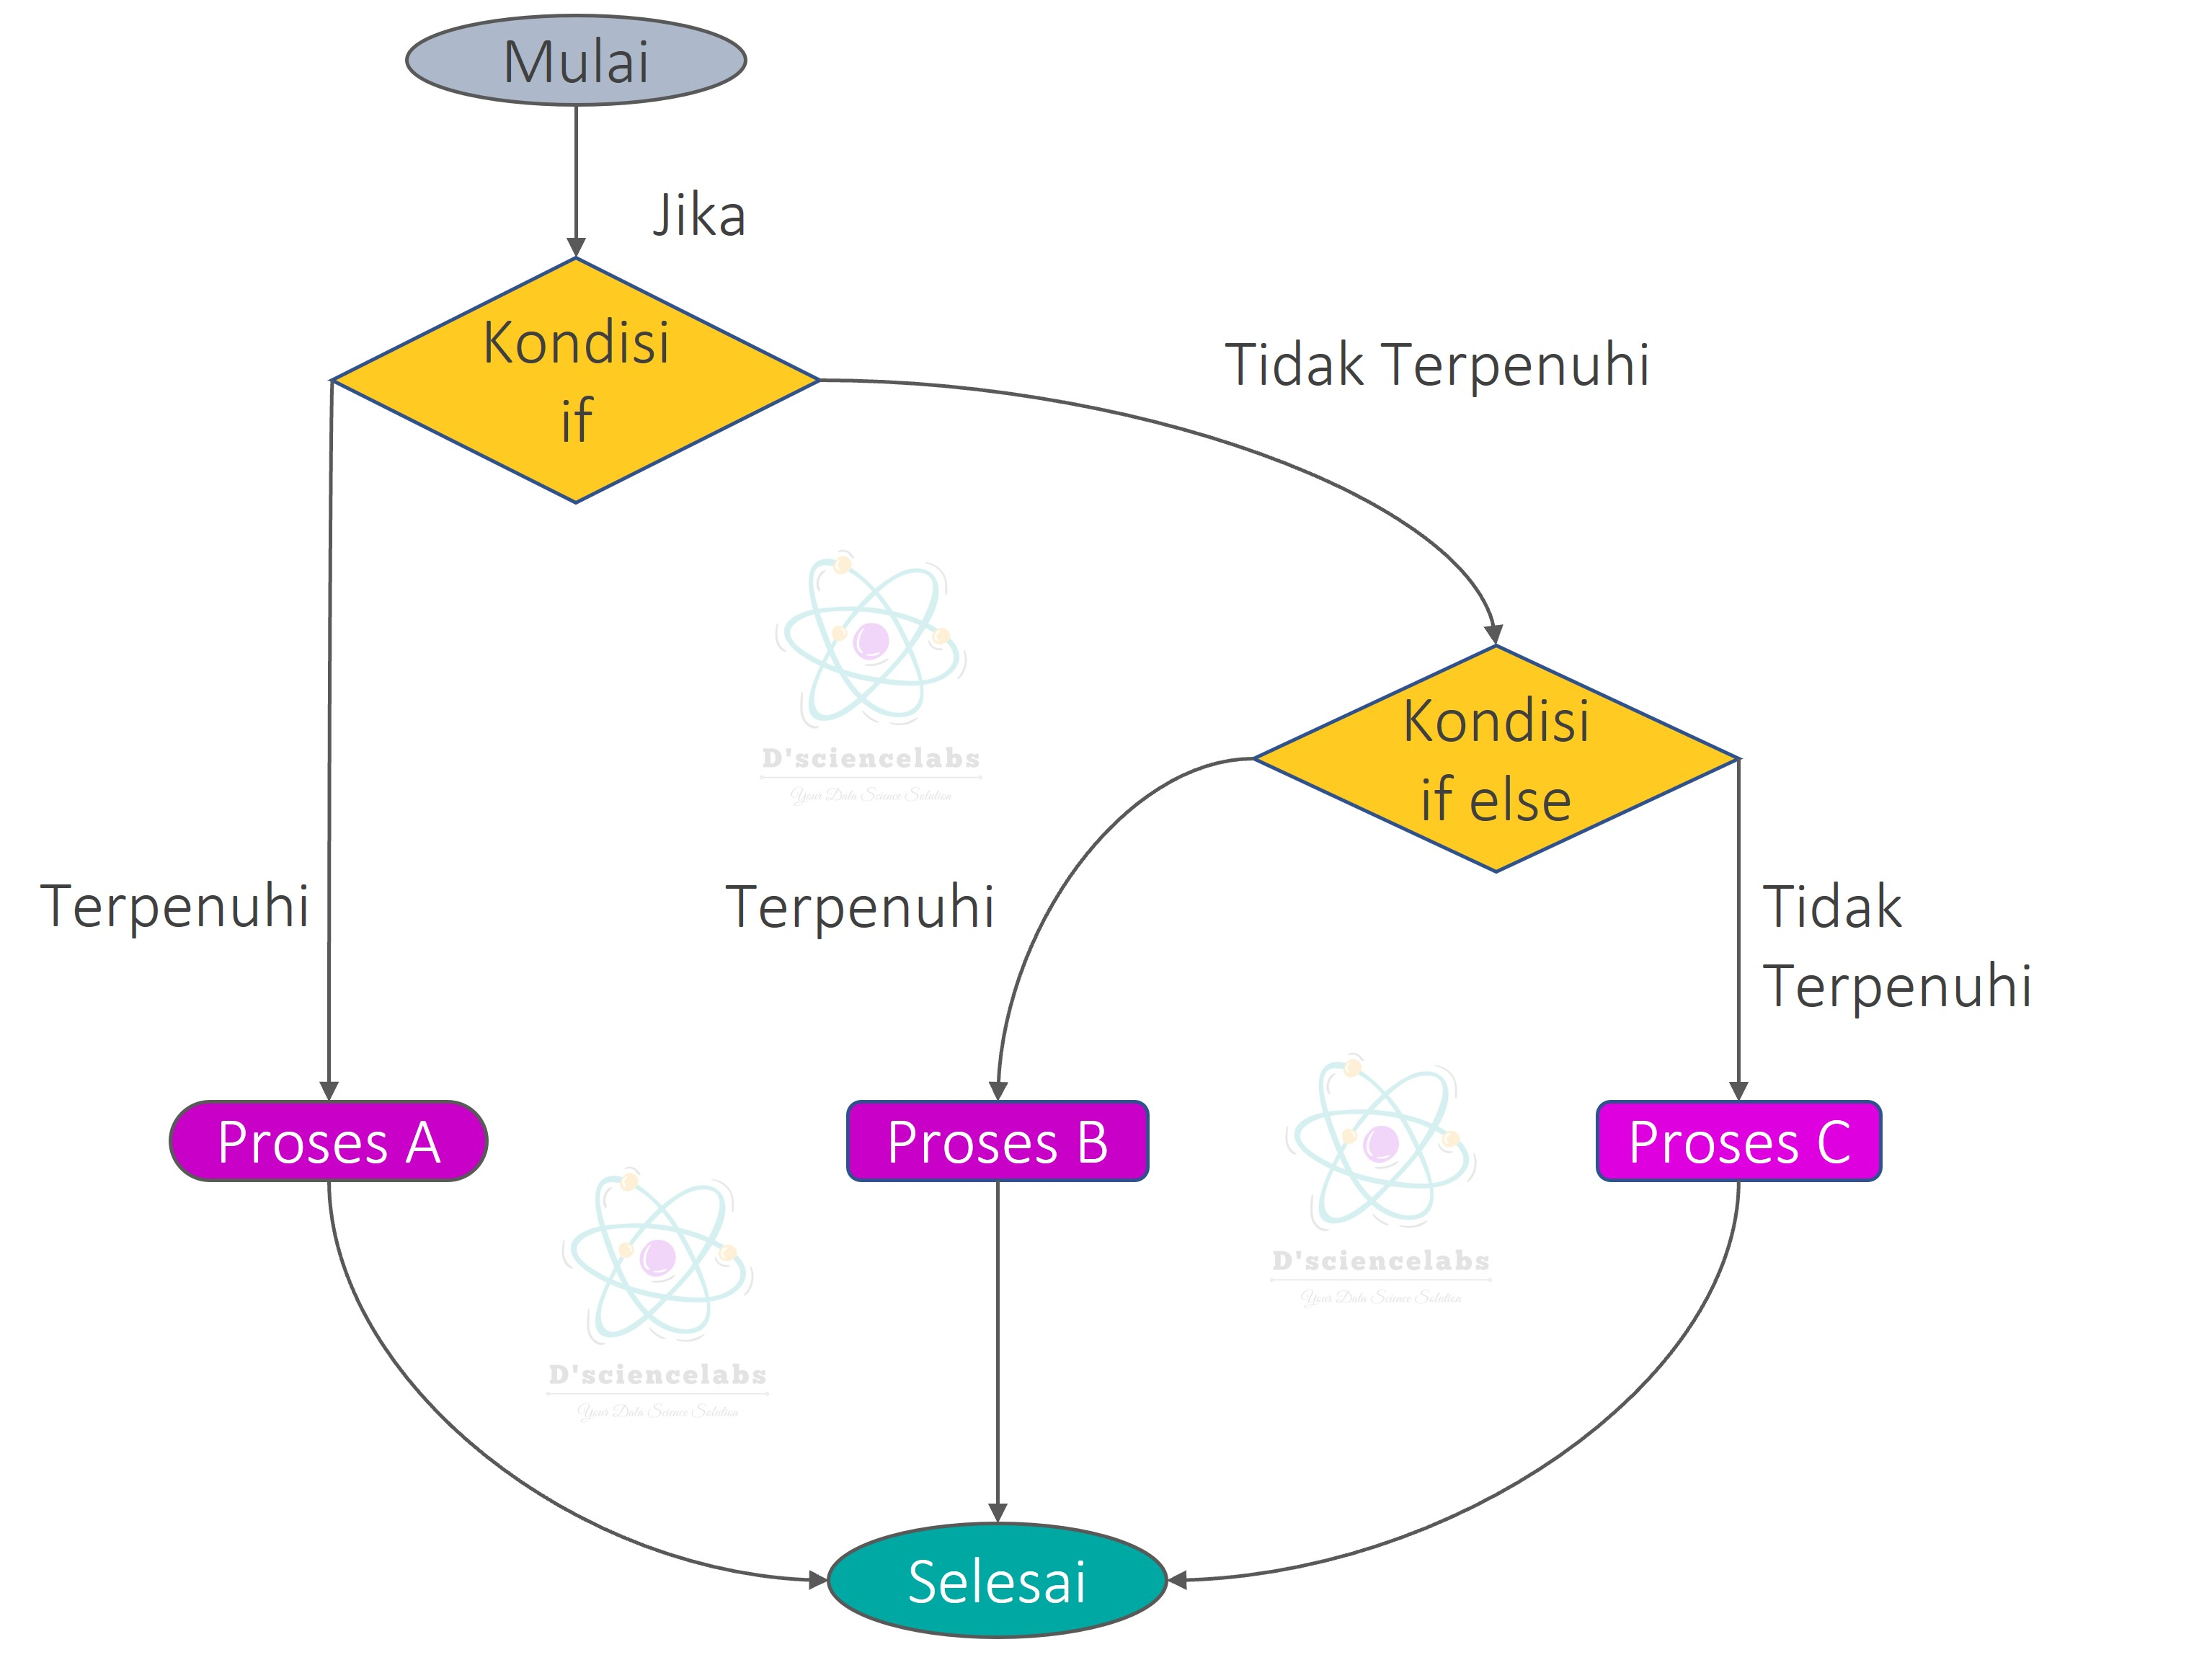
\includegraphics[width=1\linewidth]{./images/Bab6/if-else} 

}

\caption{Struktur Kontrol if else}\label{fig:if-else}
\end{figure}

\hypertarget{sintaks-if-else-if-dan-else}{%
\subsection{\texorpdfstring{Sintaks \texttt{if,\ else-if}, dan \texttt{else}}{Sintaks if, else-if, dan else}}\label{sintaks-if-else-if-dan-else}}

Secara garis besar struktur kontrol pengambilan keputasan yang paling umum digunakan dalam bahasa pemrograman R adalah kombinasi \texttt{if-else}, bahkan untuk semua bahasa pemrograman lainnya. Struktur kontrol ini memungkinkan untuk menguji suatu kondisi dan menindaklanjutinya tergantung pada apakah itu benar atau salah.

Anda dapat memiliki serangkaian tes dengan mengikuti inisial \texttt{if} dengan sejumlah \texttt{else\ if} dan \texttt{else} itu sendiri. Fungsi umum untuk ini, seperti kode berikut:

\begin{verbatim}
nama.fungsi <- function(argumen){
  if (kondisi1) {
      lakukan sesuatu 
      } 
  else if (kondisi2) {
      lakukan sesuatu yang berbeda dibandingkan dengan kondisi 1} 
  else if (kondisi3) {
      lakukan sesuatu yang berbeda dibandingkan dengan kondisi 1,2} 
  else if (kondisi4) {
      lakukan sesuatu yang berbeda dibandingkan dengan kondisi 1,2,3} 
  else (opsional){
      melakukan sesuatu yang berbeda dibandingkan semua kondisi semua}
}
\end{verbatim}

\hypertarget{program-penilaian}{%
\subsection{Program Penilaian}\label{program-penilaian}}

Andaikan anda ingin membuat suatu program yang dapat memudahkan anda untuk memberikan peringkat kepada nilai mahasiswa sesuai dengan standar yang berlaku. Perhatikan contoh berikut dalam R:

\begin{Shaded}
\begin{Highlighting}[]
\NormalTok{x }\OtherTok{\textless{}{-}} \FunctionTok{runif}\NormalTok{(}\DecValTok{1}\NormalTok{, }\DecValTok{50}\NormalTok{, }\DecValTok{100}\NormalTok{)                      }\CommentTok{\# pilih satu nomor acak dari 0\textasciitilde{}100}
\NormalTok{nilai }\OtherTok{\textless{}{-}} \ControlFlowTok{function}\NormalTok{(x)\{}
            \ControlFlowTok{if}\NormalTok{ (x}\SpecialCharTok{\textgreater{}=}\DecValTok{85}\NormalTok{)\{                     }\CommentTok{\# kondisi 1}
              \FunctionTok{print}\NormalTok{(}\StringTok{\textquotesingle{}Peringkat A\textquotesingle{}}\NormalTok{)\}         }\CommentTok{\# hasil untuk kondisi 1 }
            \ControlFlowTok{else} \ControlFlowTok{if}\NormalTok{ (x}\SpecialCharTok{\textless{}}\DecValTok{85} \SpecialCharTok{\&}\NormalTok{ x }\SpecialCharTok{\textgreater{}=}\DecValTok{70}\NormalTok{)\{        }\CommentTok{\# kondisi 2 }
              \FunctionTok{print}\NormalTok{(}\StringTok{\textquotesingle{}Peringkat B\textquotesingle{}}\NormalTok{)\}         }\CommentTok{\# hasil untuk kondisi 2}
            \ControlFlowTok{else} \ControlFlowTok{if}\NormalTok{ (x}\SpecialCharTok{\textless{}=}\DecValTok{69} \SpecialCharTok{\&}\NormalTok{ x }\SpecialCharTok{\textgreater{}=}\DecValTok{60}\NormalTok{)\{       }\CommentTok{\# kondisi 3 }
              \FunctionTok{print}\NormalTok{(}\StringTok{\textquotesingle{}Peringkat C\textquotesingle{}}\NormalTok{)\}         }\CommentTok{\# hasil untuk kondisi 3}
            \ControlFlowTok{else} \ControlFlowTok{if}\NormalTok{ (x}\SpecialCharTok{\textless{}=}\DecValTok{59} \SpecialCharTok{\&}\NormalTok{ x }\SpecialCharTok{\textgreater{}=}\DecValTok{50}\NormalTok{)\{       }\CommentTok{\# kondisi 4 }
              \FunctionTok{print}\NormalTok{(}\StringTok{\textquotesingle{}Peringkat D\textquotesingle{}}\NormalTok{)\}         }\CommentTok{\# hasil untuk kondisi 4}
            \ControlFlowTok{else}\NormalTok{\{                           }\CommentTok{\# kondisi 5}
              \FunctionTok{print}\NormalTok{(}\StringTok{\textquotesingle{}Gagal\textquotesingle{}}\NormalTok{)\}               }\CommentTok{\# hasil untuk kondisi 5}
\NormalTok{\}}
\FunctionTok{nilai}\NormalTok{(x)}
\end{Highlighting}
\end{Shaded}

\begin{verbatim}
## [1] "Peringkat C"
\end{verbatim}

\hypertarget{program-hitung-faktorial}{%
\subsection{Program Hitung Faktorial}\label{program-hitung-faktorial}}

Untuk menambah pemahaman terkait pengambilan keputusan dalam pemrograman, mari kita perhatiakan contoh berikut: fungsi factorial menghitung faktorial dari suatu bilangan n.

\begin{Shaded}
\begin{Highlighting}[]
\NormalTok{factorial }\OtherTok{\textless{}{-}} \ControlFlowTok{function}\NormalTok{(n) \{}
  \ControlFlowTok{if}\NormalTok{ (n }\SpecialCharTok{==} \DecValTok{0} \SpecialCharTok{||}\NormalTok{ n }\SpecialCharTok{==} \DecValTok{1}\NormalTok{) \{}
    \FunctionTok{return}\NormalTok{(}\DecValTok{1}\NormalTok{)}
\NormalTok{  \} }\ControlFlowTok{else}\NormalTok{ \{}
    \FunctionTok{return}\NormalTok{(n }\SpecialCharTok{*} \FunctionTok{factorial}\NormalTok{(n }\SpecialCharTok{{-}} \DecValTok{1}\NormalTok{))}
\NormalTok{  \}}
\NormalTok{\}}

\NormalTok{result }\OtherTok{\textless{}{-}} \FunctionTok{factorial}\NormalTok{(}\DecValTok{5}\NormalTok{)}
\FunctionTok{print}\NormalTok{(result)  }\CommentTok{\# Output: 120}
\end{Highlighting}
\end{Shaded}

\begin{verbatim}
## [1] 120
\end{verbatim}

Faktorial dari n (dilambangkan sebagai n!) adalah hasil perkalian semua bilangan bulat positif dari 1 hingga n.~Dalam implementasi tersebut, fungsi factorial memanggil dirinya sendiri dengan argumen yang lebih kecil hingga mencapai kasus dasar (n = 0 atau n = 1), di mana hasil faktorialnya adalah 1.

Namun, perlu diingat bahwa pengulangan rekursif dapat menyebabkan pemanggilan berulang yang dalam beberapa kasus dapat mengakibatkan penumpukan memori (stack overflow) atau kinerja yang buruk. Oleh karena itu, perlu dipastikan bahwa ada kondisi berhenti yang jelas untuk menghindari pengulangan tak terbatas. Selain itu, dalam beberapa situasi, solusi non-rekursif atau pendekatan lain mungkin lebih efisien.

\hypertarget{pengulangan-rekursif}{%
\section{Pengulangan Rekursif}\label{pengulangan-rekursif}}

Pada saat melakukan analisis data, terkadang seorang data analis atau data scientist perlu menggunakan fungsi pengulangan dalam proses pembentukan, perhitungan, manipulasi struktur data seperti halnya vektor, matriks, list, data frame, atau objek lainnya.

\hypertarget{sintaks-for}{%
\subsection{\texorpdfstring{Sintaks \texttt{for}}{Sintaks for}}\label{sintaks-for}}

Dalam porose perulangan ini digunakan fungsi kontrol `for', dimana setiap iterasi pada beberapa perintah akan dievaluasi melalui perulangan yang diinginkan.

\begin{figure}

{\centering 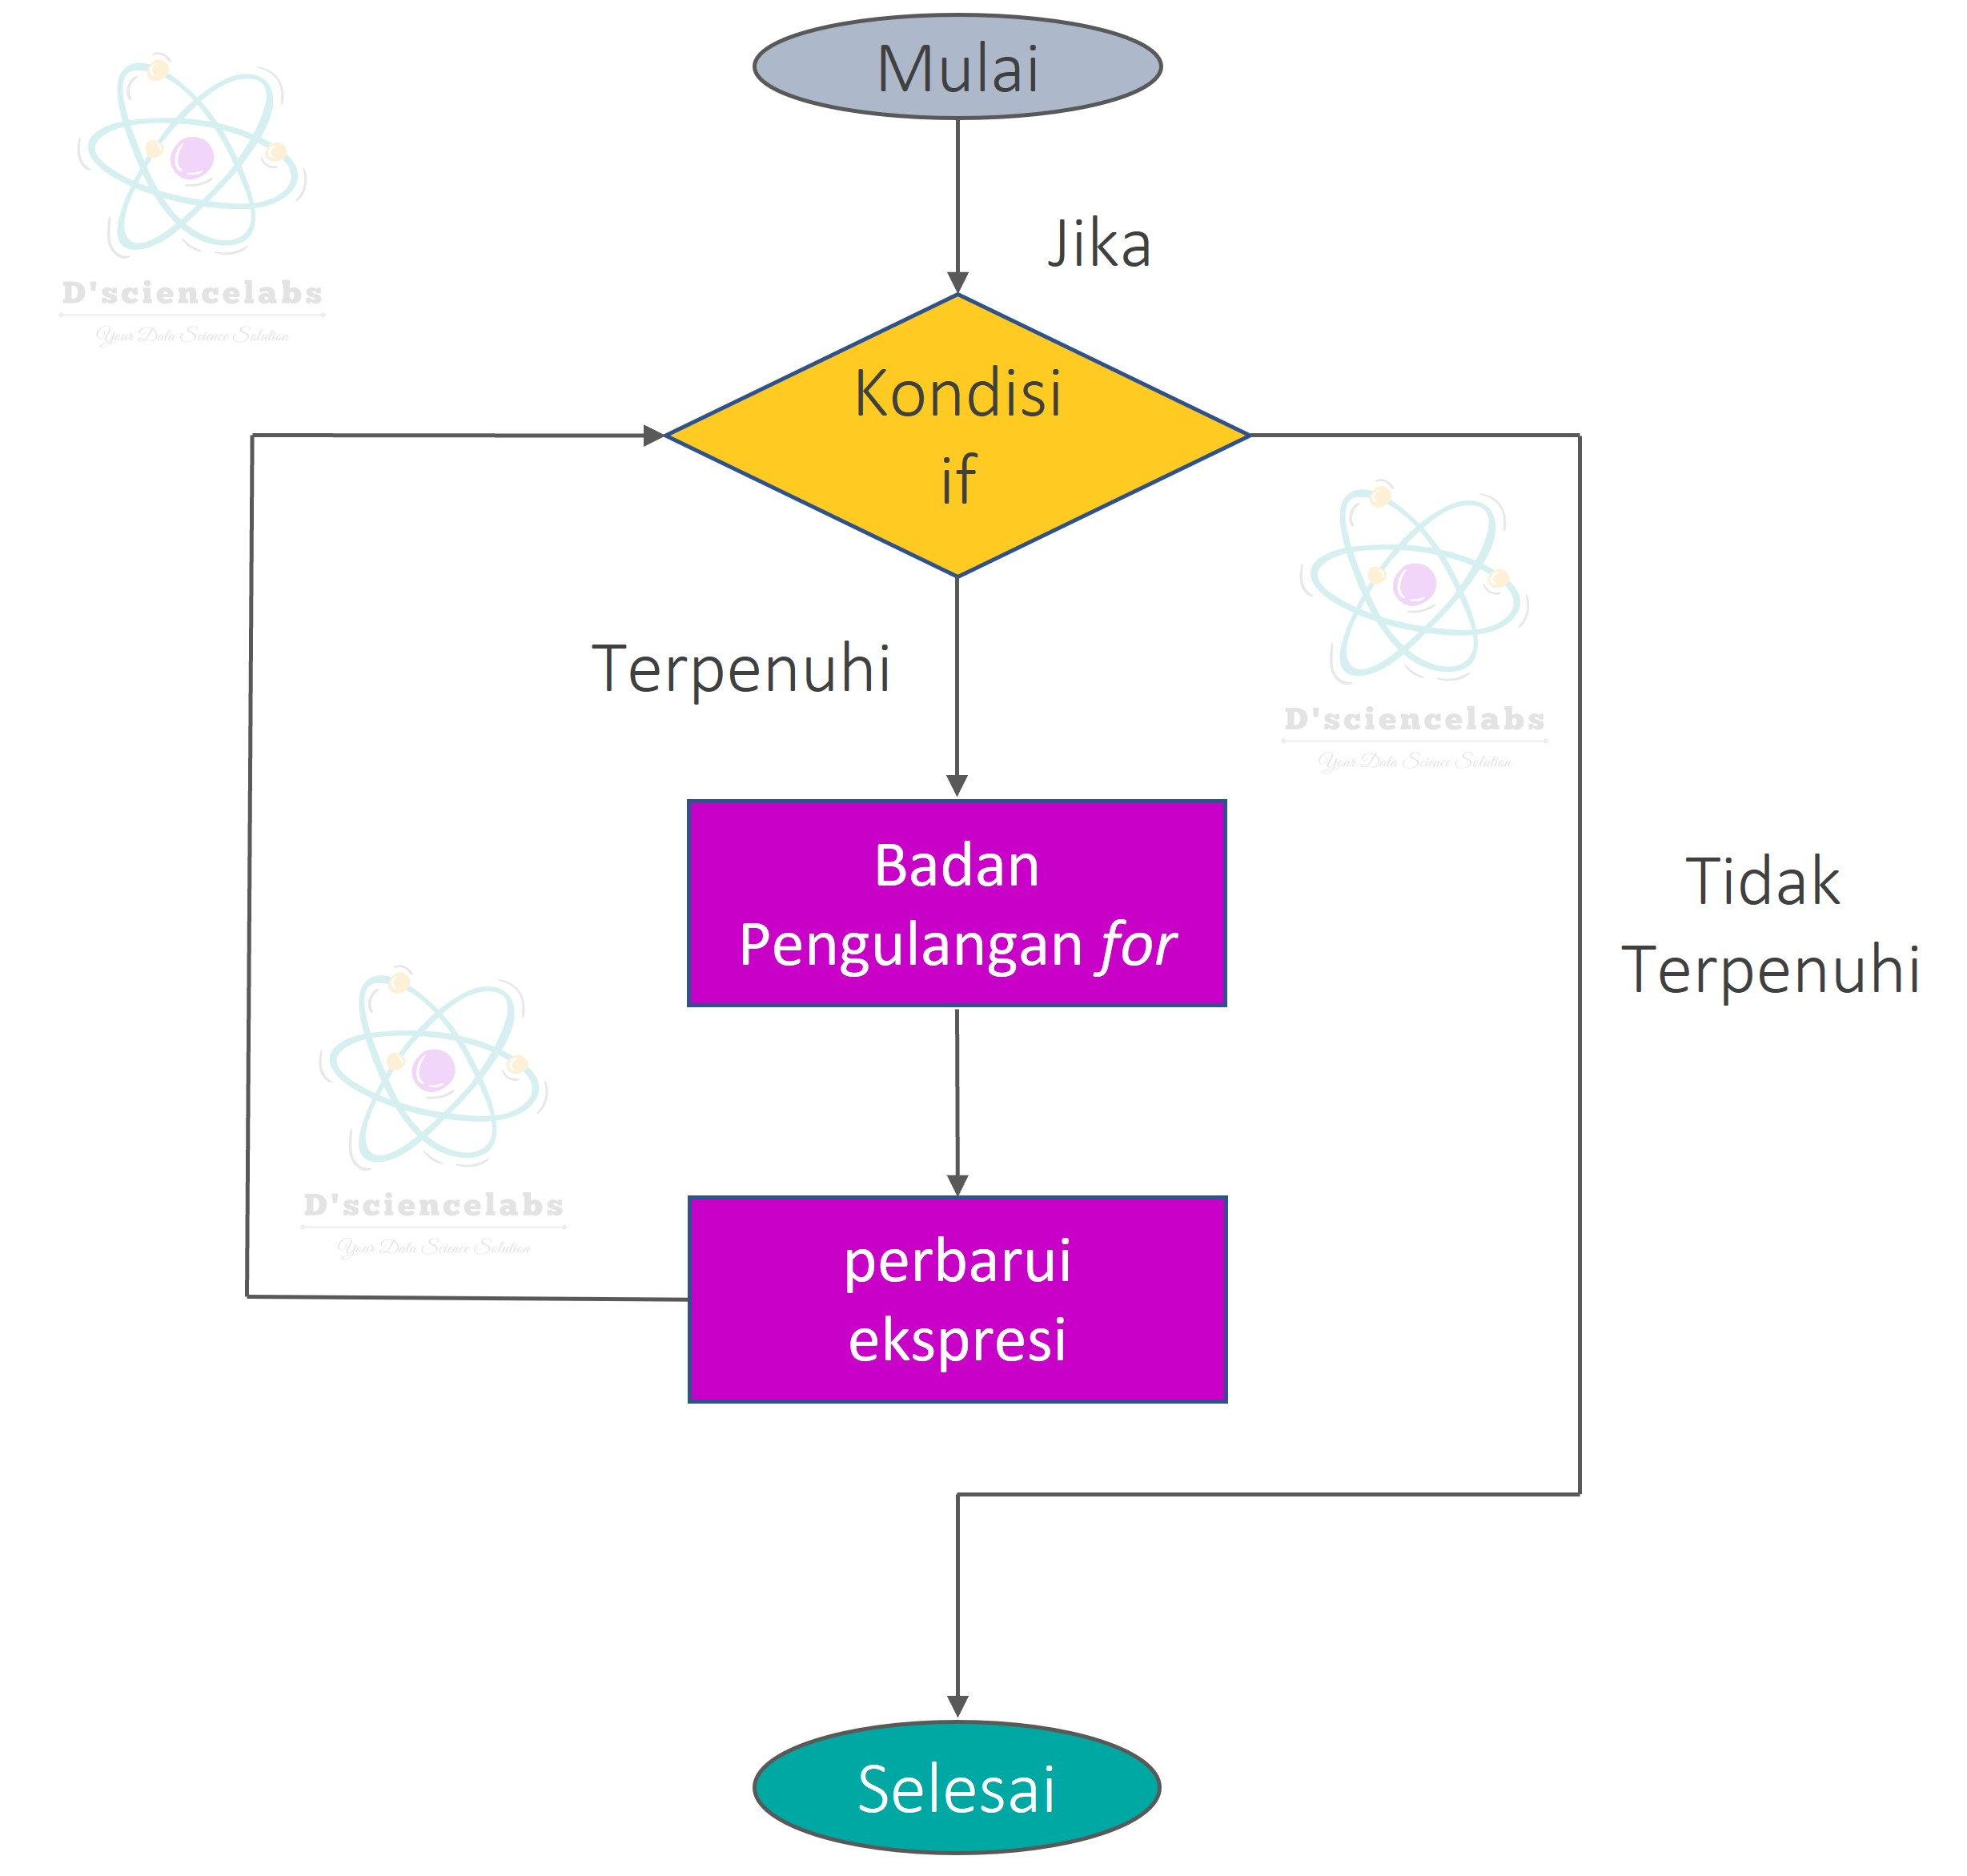
\includegraphics[width=1\linewidth]{./images/Bab6/for} 

}

\caption{Struktur Kontrol for}\label{fig:for}
\end{figure}

Pada gambar di atas bisa dilihat bahwa perulangan juga memerlukan tes kondisi. Bila hasil tes kondisi terpenuhi, maka blok kode kembali dieksekusi. Tapi jika tidak terpenuhi, maka keluar dari perulangan. Sintaks pengulangan for di R sangat sederhana, dapat diperlihatkan sebagai berikut:

\begin{verbatim}
For (i in vector) {
    lakukan sesuatu     
}
\end{verbatim}

Jika anda ingin mencetak \(i + 1\), menjadi \(i = 1,\cdots 10,\) pada setiap iterasi pengulangan (loop). Anda dapat menggunakan sintaks \texttt{for} untuk mencetak angka dengan yang dimulai \(i = 0\) dan berakhir pada \(i = 10\), sebagai berikut:

\begin{Shaded}
\begin{Highlighting}[]
\ControlFlowTok{for}\NormalTok{ (i }\ControlFlowTok{in} \DecValTok{0}\SpecialCharTok{:}\DecValTok{10}\NormalTok{) \{}
  \FunctionTok{print}\NormalTok{(i }\SpecialCharTok{+} \DecValTok{1}\NormalTok{)}
\NormalTok{\}}
\end{Highlighting}
\end{Shaded}

\begin{verbatim}
## [1] 1
## [1] 2
## [1] 3
## [1] 4
## [1] 5
## [1] 6
## [1] 7
## [1] 8
## [1] 9
## [1] 10
## [1] 11
\end{verbatim}

Selain dapat digunakan pada data numerik, pengulangan for ini dapat juga diterapkan pada data karakter sebagai berikut:

\begin{Shaded}
\begin{Highlighting}[]
\NormalTok{mapel }\OtherTok{=} \FunctionTok{c}\NormalTok{(}\StringTok{\textquotesingle{}Data Science\textquotesingle{}}\NormalTok{, }\StringTok{\textquotesingle{}Statistika\textquotesingle{}}\NormalTok{,}\StringTok{\textquotesingle{}Algoritma dan Pemrograman\textquotesingle{}}\NormalTok{)}

\ControlFlowTok{for}\NormalTok{ (i }\ControlFlowTok{in}\NormalTok{ mapel)\{}
   \FunctionTok{print}\NormalTok{(}\FunctionTok{paste0}\NormalTok{(}\StringTok{"Saya suka: "}\NormalTok{, i))}
\NormalTok{\}}
\end{Highlighting}
\end{Shaded}

\begin{verbatim}
## [1] "Saya suka: Data Science"
## [1] "Saya suka: Statistika"
## [1] "Saya suka: Algoritma dan Pemrograman"
\end{verbatim}

Selain itu, anda juga dapat melakukan pengulangan bersarang untuk siklus tertentu. Sintaksnya direpresentasikan sebagai berikut:

\begin{Shaded}
\begin{Highlighting}[]
\NormalTok{nama }\OtherTok{=} \FunctionTok{c}\NormalTok{(}\StringTok{"Bakti: "}\NormalTok{, }\StringTok{"Alexander: "}\NormalTok{, }\StringTok{"Siregar: "}\NormalTok{)}
\NormalTok{mapel }\OtherTok{=} \FunctionTok{c}\NormalTok{(}\StringTok{\textquotesingle{}Data Science\textquotesingle{}}\NormalTok{, }\StringTok{\textquotesingle{}Statistika\textquotesingle{}}\NormalTok{,}\StringTok{\textquotesingle{}Algoritma dan Pemrograman\textquotesingle{}}\NormalTok{)}

\ControlFlowTok{for}\NormalTok{ (x }\ControlFlowTok{in}\NormalTok{ nama)}
  \ControlFlowTok{for}\NormalTok{ (y }\ControlFlowTok{in}\NormalTok{ mapel)\{}
    \FunctionTok{print}\NormalTok{(}\FunctionTok{paste0}\NormalTok{(x, y))}
\NormalTok{  \}}
\end{Highlighting}
\end{Shaded}

\begin{verbatim}
## [1] "Bakti: Data Science"
## [1] "Bakti: Statistika"
## [1] "Bakti: Algoritma dan Pemrograman"
## [1] "Alexander: Data Science"
## [1] "Alexander: Statistika"
## [1] "Alexander: Algoritma dan Pemrograman"
## [1] "Siregar: Data Science"
## [1] "Siregar: Statistika"
## [1] "Siregar: Algoritma dan Pemrograman"
\end{verbatim}

\hypertarget{sintaks-while}{%
\subsection{\texorpdfstring{Sintaks \texttt{while}}{Sintaks while}}\label{sintaks-while}}

Terkadang anda bahkan tidak tahu berapa lama urutan input harus dijalankan. Hal ini biasa terjadi saat melakukan simulasi. Misalnya, Anda mungkin ingin mengulang sampai anda mendapatkan tiga kepala berturut-turut. Anda tidak dapat melakukan iterasi semacam itu dengan pengulangan \texttt{for}. Sebagai gantinya, Anda dapat menggunakan pengulangan \texttt{while}. Perulangan \texttt{while} lebih sederhana daripada perulangan for karena hanya memiliki dua komponen, kondisi, dan badan.

\begin{figure}

{\centering 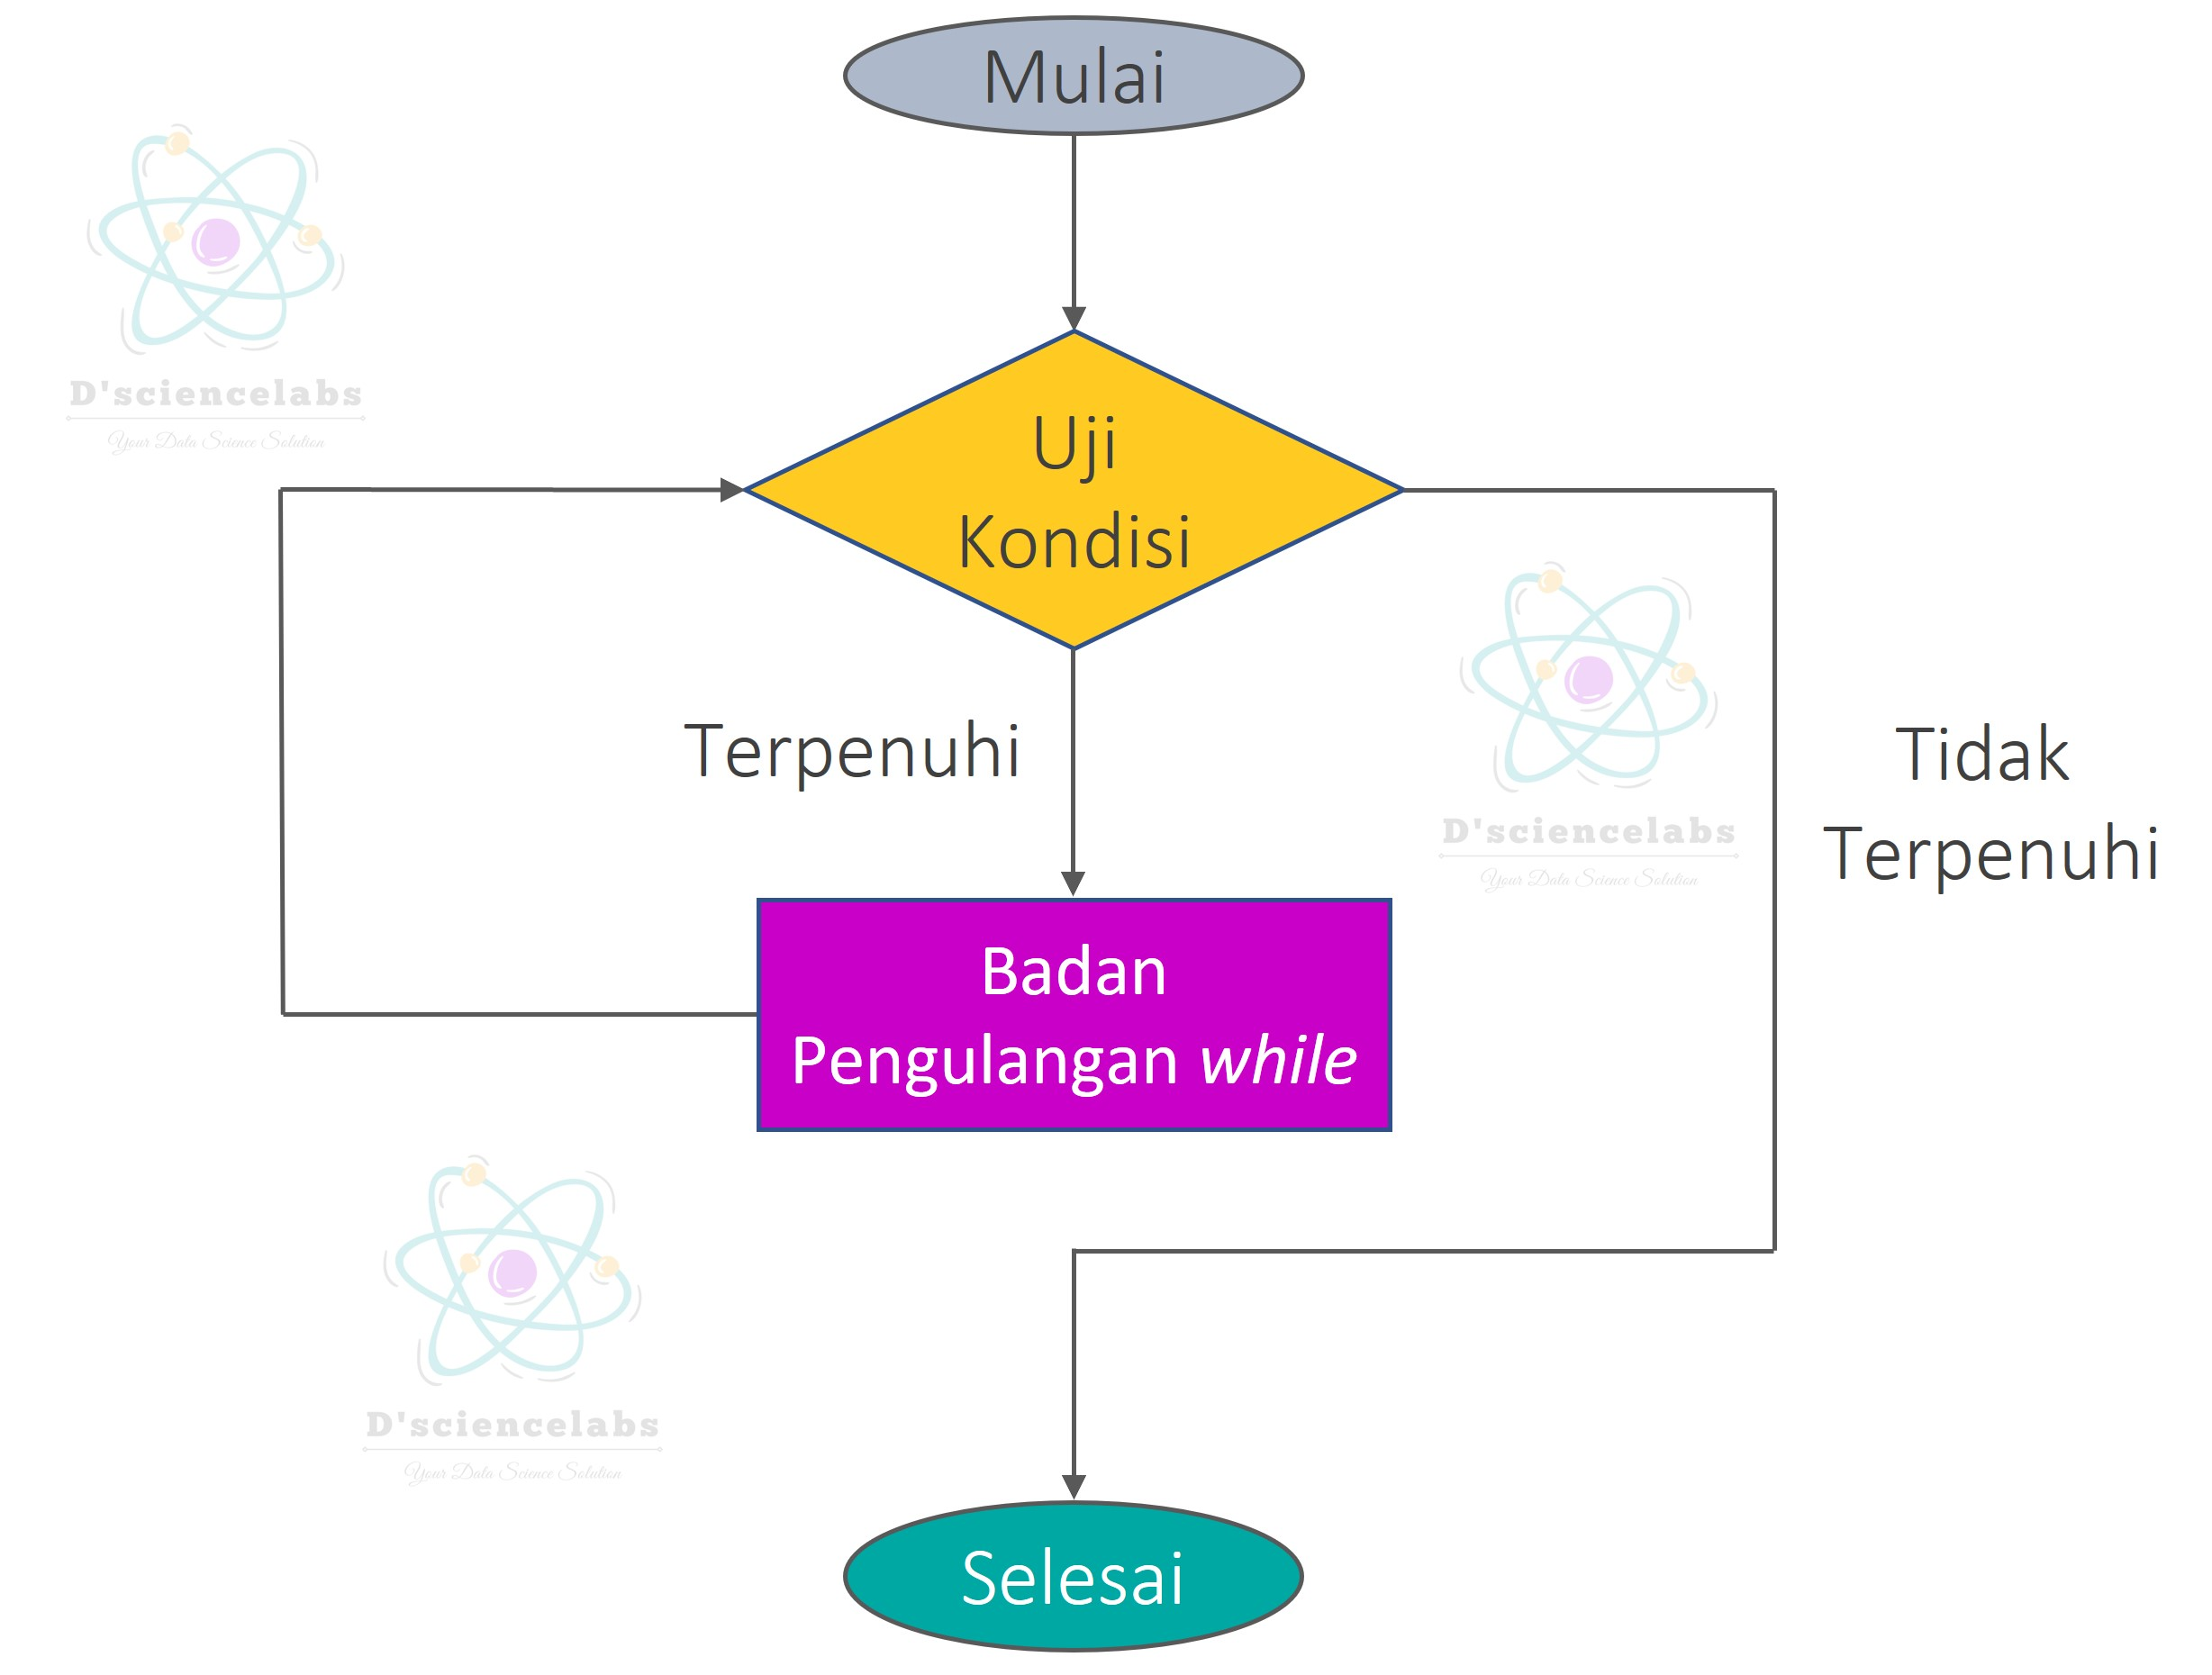
\includegraphics[width=1\linewidth]{./images/Bab6/while} 

}

\caption{Struktur Kontrol while}\label{fig:while}
\end{figure}

Perulangan \texttt{while} dimulai dengan menguji suatu kondisi. Jika benar, maka mereka mengeksekusi badan perulangan. Setelah tubuh loop dieksekusi, kondisinya diuji lagi, dan seterusnya, sampai kondisinya salah, setelah itu loop akan melakukan eksekusi pada kodisi lainnya jika ada. Sintaks untuk \texttt{while} loop adalah sebagai berikut:

\begin{verbatim}
while (Kondisi) {
     lakukan sesuatu 
}
\end{verbatim}

Pengulangan while dalam bahasa pemrograman R digunakan untuk menjalankan serangkaian pernyataan selama kondisi tertentu tetap terpenuhi. Berikut adalah contoh penggunaan pengulangan while dalam R:

\begin{Shaded}
\begin{Highlighting}[]
\NormalTok{x }\OtherTok{\textless{}{-}} \DecValTok{1}

\ControlFlowTok{while}\NormalTok{ (x }\SpecialCharTok{\textless{}=} \DecValTok{5}\NormalTok{) \{}
  \FunctionTok{print}\NormalTok{(x)}
\NormalTok{  x }\OtherTok{\textless{}{-}}\NormalTok{ x }\SpecialCharTok{+} \DecValTok{1}
\NormalTok{\}}
\end{Highlighting}
\end{Shaded}

\begin{verbatim}
## [1] 1
## [1] 2
## [1] 3
## [1] 4
## [1] 5
\end{verbatim}

Dalam contoh di atas, loop while akan menjalankan blok pernyataan selama nilai x masih kurang dari atau sama dengan 5. Setiap kali loop dijalankan, nilai x akan ditambah 1, sehingga pada akhirnya, kondisi x \textless= 5 akan menjadi salah dan loop akan berhenti.

Anda perlu memastikan bahwa ada pernyataan di dalam blok while yang mengubah nilai yang digunakan dalam kondisi. Ini penting untuk menghindari terjebak dalam loop tak berakhir.

Berikut adalah contoh lain dengan menggunakan pengulangan while untuk menghitung jumlah bilangan genap antara 1 dan 10:

\begin{Shaded}
\begin{Highlighting}[]
\NormalTok{count }\OtherTok{\textless{}{-}} \DecValTok{1}
\NormalTok{even\_sum }\OtherTok{\textless{}{-}} \DecValTok{0}

\ControlFlowTok{while}\NormalTok{ (count }\SpecialCharTok{\textless{}=} \DecValTok{10}\NormalTok{) \{}
  \ControlFlowTok{if}\NormalTok{ (count }\SpecialCharTok{\%\%} \DecValTok{2} \SpecialCharTok{==} \DecValTok{0}\NormalTok{) \{}
\NormalTok{    even\_sum }\OtherTok{\textless{}{-}}\NormalTok{ even\_sum }\SpecialCharTok{+}\NormalTok{ count}
\NormalTok{  \}}
\NormalTok{  count }\OtherTok{\textless{}{-}}\NormalTok{ count }\SpecialCharTok{+} \DecValTok{1}
\NormalTok{\}}

\FunctionTok{print}\NormalTok{(even\_sum)  }\CommentTok{\# Output: 30 (2 + 4 + 6 + 8 + 10)}
\end{Highlighting}
\end{Shaded}

\begin{verbatim}
## [1] 30
\end{verbatim}

Dalam contoh ini, kita menggunakan loop while untuk menghitung jumlah bilangan genap antara 1 dan 10. Kita memeriksa apakah count (bilangan saat ini) adalah bilangan genap dengan menggunakan operator modulo (\%\%). Jika ya, kita menambahkan bilangan tersebut ke even\_sum.

Penting untuk selalu memastikan bahwa kondisi dalam loop while pada suatu titik akan menjadi salah, sehingga loop akan berhenti dan program tidak terjebak dalam perulangan tak berakhir.

\hypertarget{interupsi-pengulangan}{%
\section{Interupsi Pengulangan}\label{interupsi-pengulangan}}

Interupsi Pengulangan dalam bahasa pemrograman dilakukan dengan pernyataan \texttt{break} pada suatu fungsi. Biasanya digunakan untuk melewati/menghentikan iterasi dan mengalirkan perintah pengulangan seperti (for, while, repeat). Meskipun, ini tidak umum digunakan dalam aplikasi statistik atau analisis data tetapi mereka memiliki peran penting dalam proses penyederhanaan program atau algoritma.

\begin{figure}

{\centering 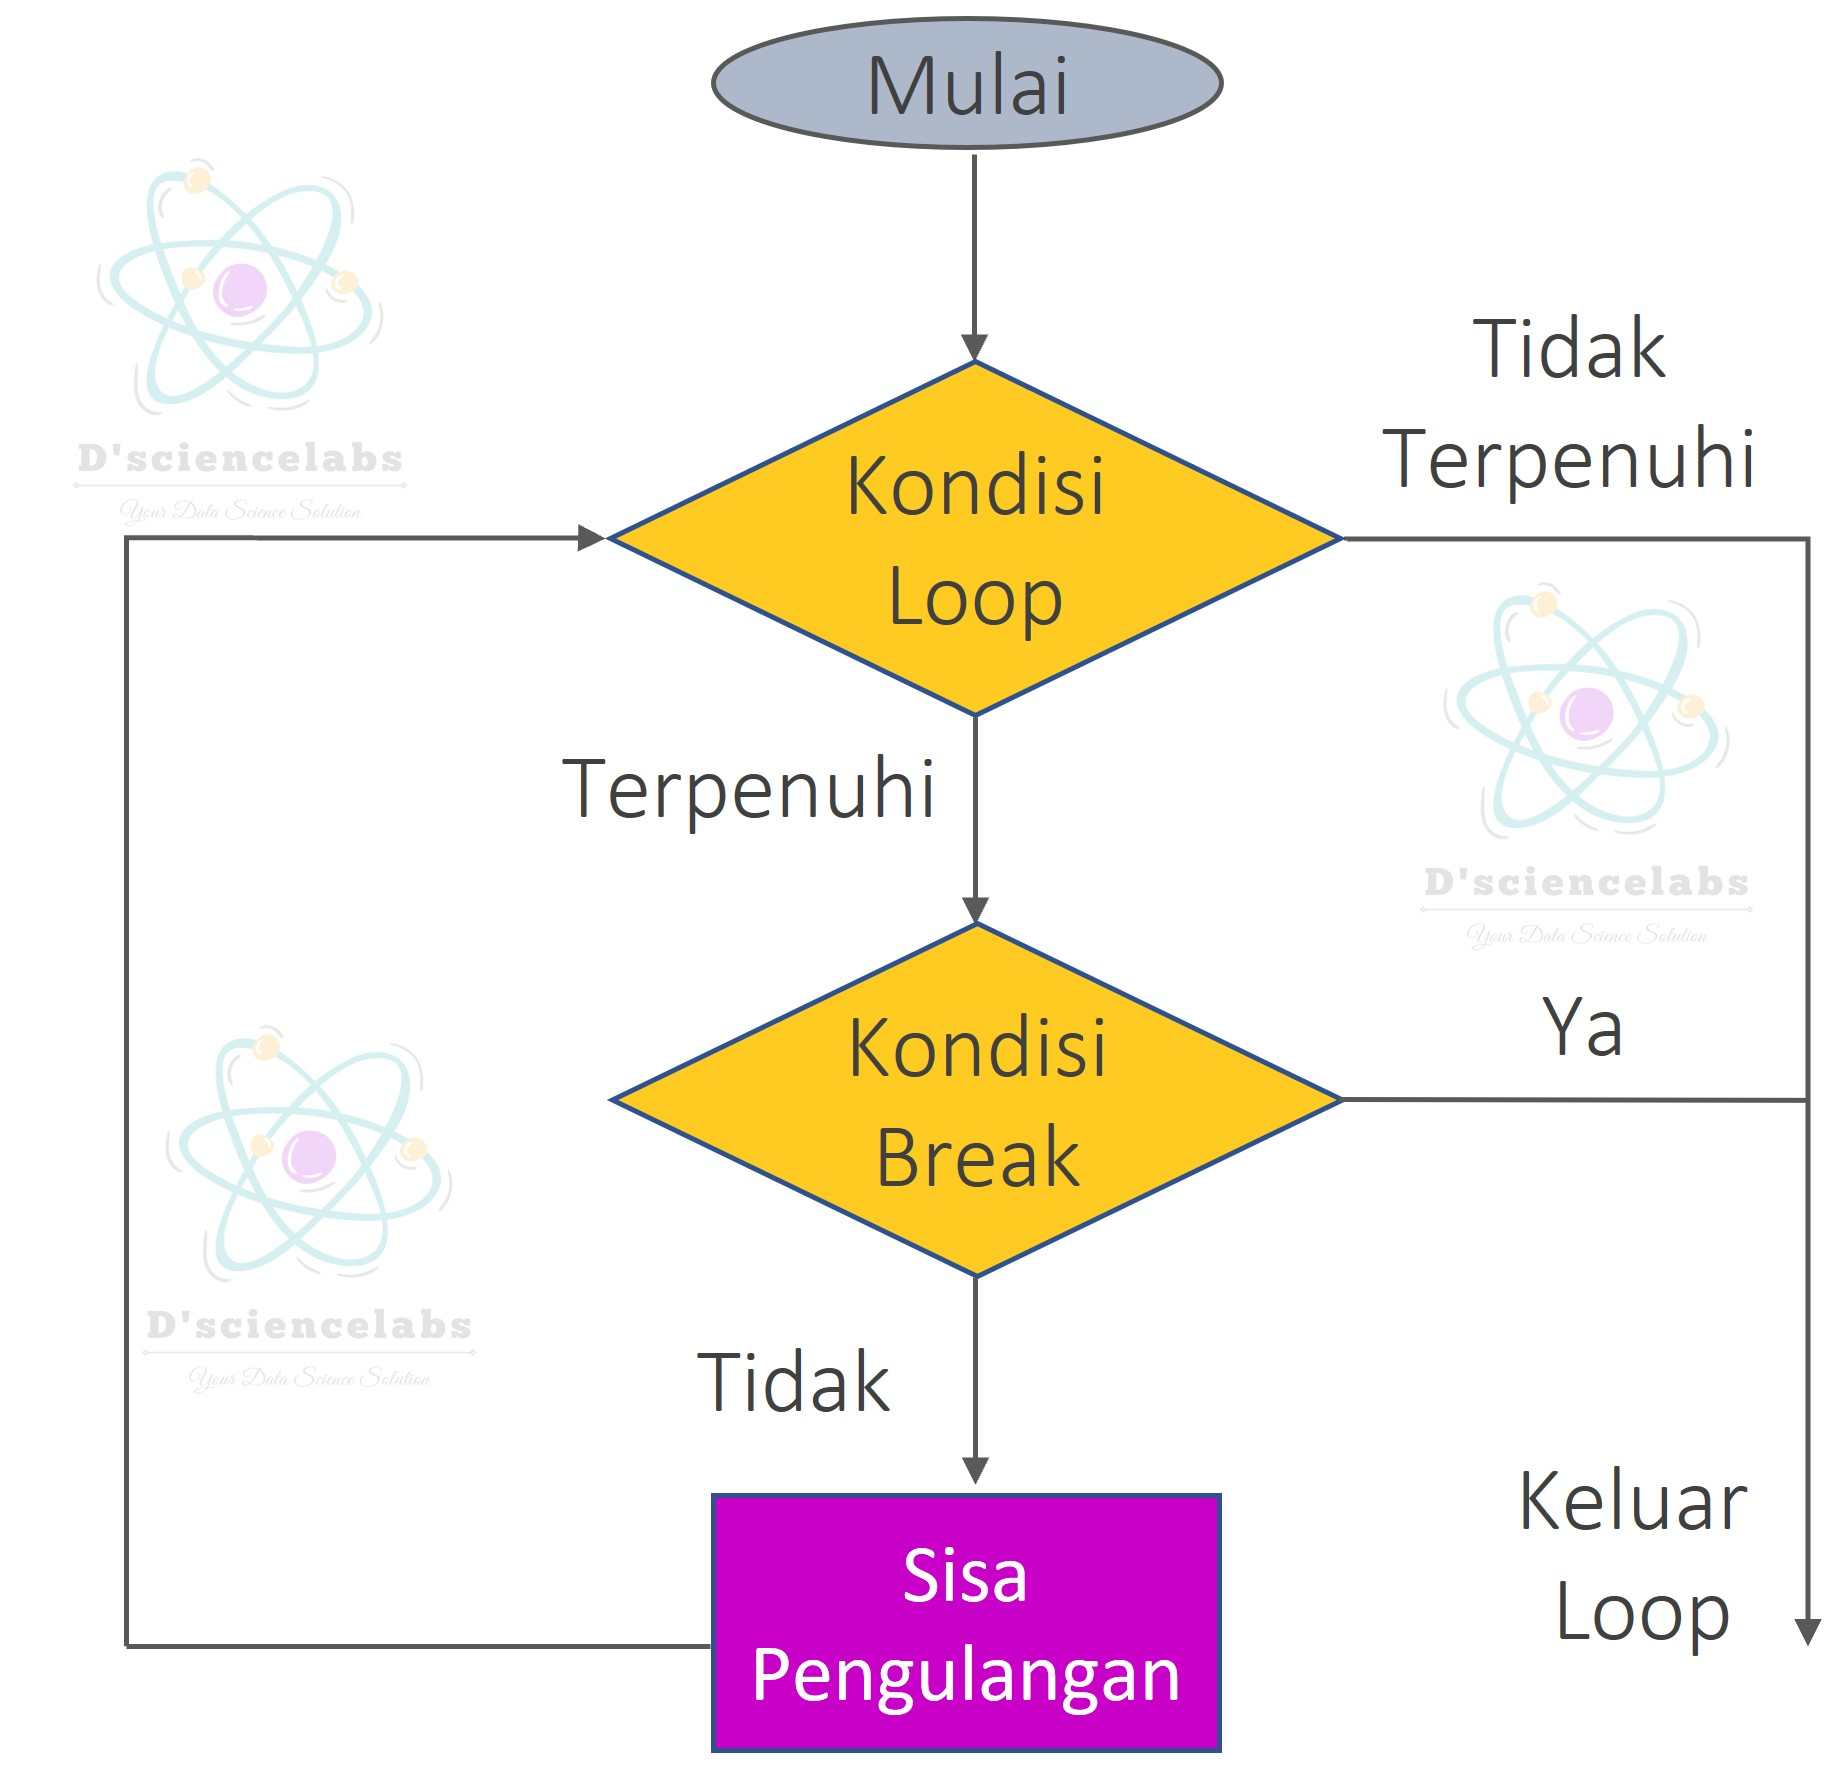
\includegraphics[width=1\linewidth]{./images/Bab6/break} 

}

\caption{Struktur Kontrol break}\label{fig:break}
\end{figure}

\begin{verbatim}
if (Test Kondisi) {
break
}
\end{verbatim}

Andaikan kita ingin melakukan pengulangan suatu nilai pada vektor x, yang memiliki angka berurutan dari 1 hingga 5. Di dalam pengulangan \texttt{for}, kita telah menggunakan kondisi \texttt{if} untuk memutuskan pengulangan pada saat ditemukan nilai sama dengan 3. Dalam hal ini, loop akan berakhir ketika sesat pernyataan break terpenuhi.

\begin{Shaded}
\begin{Highlighting}[]
\NormalTok{x }\OtherTok{\textless{}{-}} \DecValTok{1}\SpecialCharTok{:}\DecValTok{100}
\ControlFlowTok{for}\NormalTok{ (val }\ControlFlowTok{in}\NormalTok{ x) \{}
\ControlFlowTok{if}\NormalTok{ (val }\SpecialCharTok{==} \DecValTok{50}\NormalTok{)\{}
\ControlFlowTok{break}
\NormalTok{\}}
\FunctionTok{print}\NormalTok{(val)}
\NormalTok{\}}
\end{Highlighting}
\end{Shaded}

\begin{verbatim}
## [1] 1
## [1] 2
## [1] 3
## [1] 4
## [1] 5
## [1] 6
## [1] 7
## [1] 8
## [1] 9
## [1] 10
## [1] 11
## [1] 12
## [1] 13
## [1] 14
## [1] 15
## [1] 16
## [1] 17
## [1] 18
## [1] 19
## [1] 20
## [1] 21
## [1] 22
## [1] 23
## [1] 24
## [1] 25
## [1] 26
## [1] 27
## [1] 28
## [1] 29
## [1] 30
## [1] 31
## [1] 32
## [1] 33
## [1] 34
## [1] 35
## [1] 36
## [1] 37
## [1] 38
## [1] 39
## [1] 40
## [1] 41
## [1] 42
## [1] 43
## [1] 44
## [1] 45
## [1] 46
## [1] 47
## [1] 48
## [1] 49
\end{verbatim}

\hypertarget{pengulangan-berkala}{%
\section{Pengulangan Berkala}\label{pengulangan-berkala}}

Kondisi perulangan yang digunakan adalah \texttt{repeat} untuk mengulangi perintah beberapa kali. Tidak ada pemeriksaan kondisi di loop untuk keluar dalam fungsi pengulangan ini. Kita sendiri harus menempatkan kondisi secara eksplisit di dalam tubuh loop.

\begin{figure}

{\centering 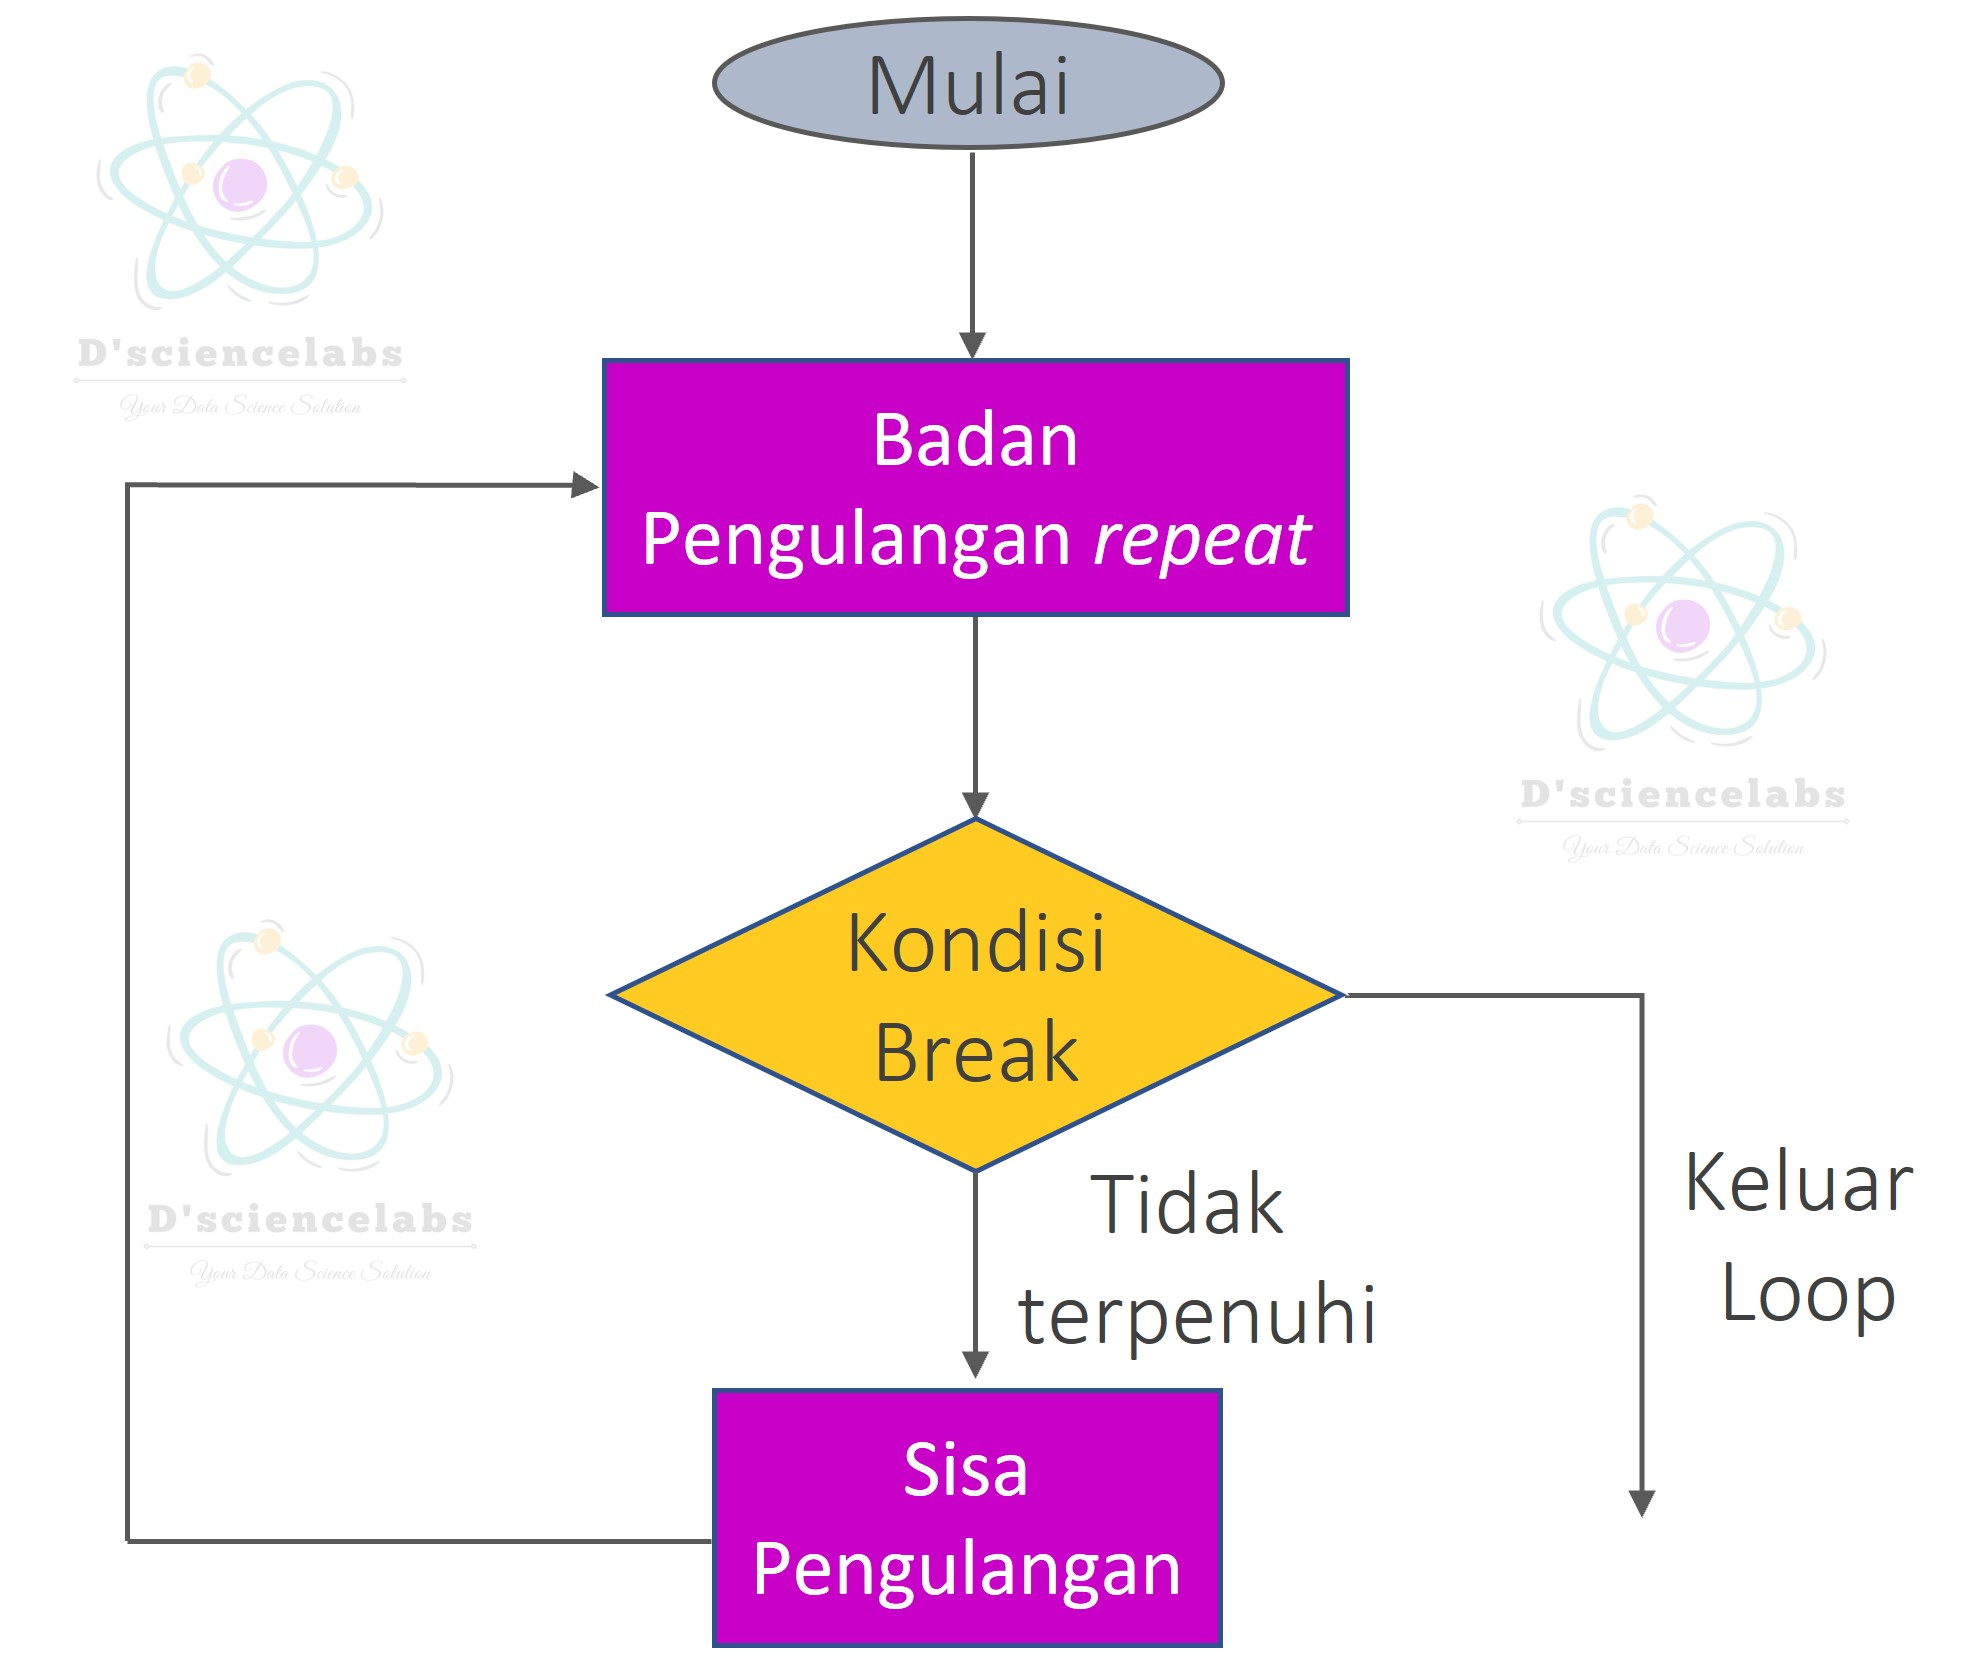
\includegraphics[width=1\linewidth]{./images/Bab6/repeat} 

}

\caption{Struktur Kontrol repeat}\label{fig:repeat}
\end{figure}

Adapun sintak yang digunakan untuk melakukan pengulangan dengan repeat adalah sebgai berikut:

\begin{verbatim}
repeat {
lakukan sesuatu
}
\end{verbatim}

Mari kita gunakan kondisi ini untuk memeriksa dan keluar dari loop ketika \(x\) mengambil nilai 6. Oleh karena itu, kita melihat dalam output bahwa hanya ada nilai dari 1 hingga 5 yang akan dicetak.

\begin{Shaded}
\begin{Highlighting}[]
\NormalTok{x }\OtherTok{\textless{}{-}} \DecValTok{1}
\ControlFlowTok{repeat}\NormalTok{ \{}
  \FunctionTok{print}\NormalTok{(x)}
\NormalTok{    x }\OtherTok{=}\NormalTok{ x}\SpecialCharTok{+}\DecValTok{1}
  \ControlFlowTok{if}\NormalTok{ (x }\SpecialCharTok{==} \DecValTok{6}\NormalTok{)\{}
  \ControlFlowTok{break}
\NormalTok{  \}}
\NormalTok{\}}
\end{Highlighting}
\end{Shaded}

\begin{verbatim}
## [1] 1
## [1] 2
## [1] 3
## [1] 4
## [1] 5
\end{verbatim}

\hypertarget{skip-iterasi-pengulangan}{%
\section{Skip Iterasi Pengulangan}\label{skip-iterasi-pengulangan}}

Penyataan skip iterasi digunakan untuk melewati sisa kode di dalam satu lingkaran untuk iterasi saat ini saja. Artinya, tidak seperti pernyataan break, pengulangan tidak berhenti tetapi terus berlanjut dengan iterasi berikutnya.

\begin{figure}

{\centering 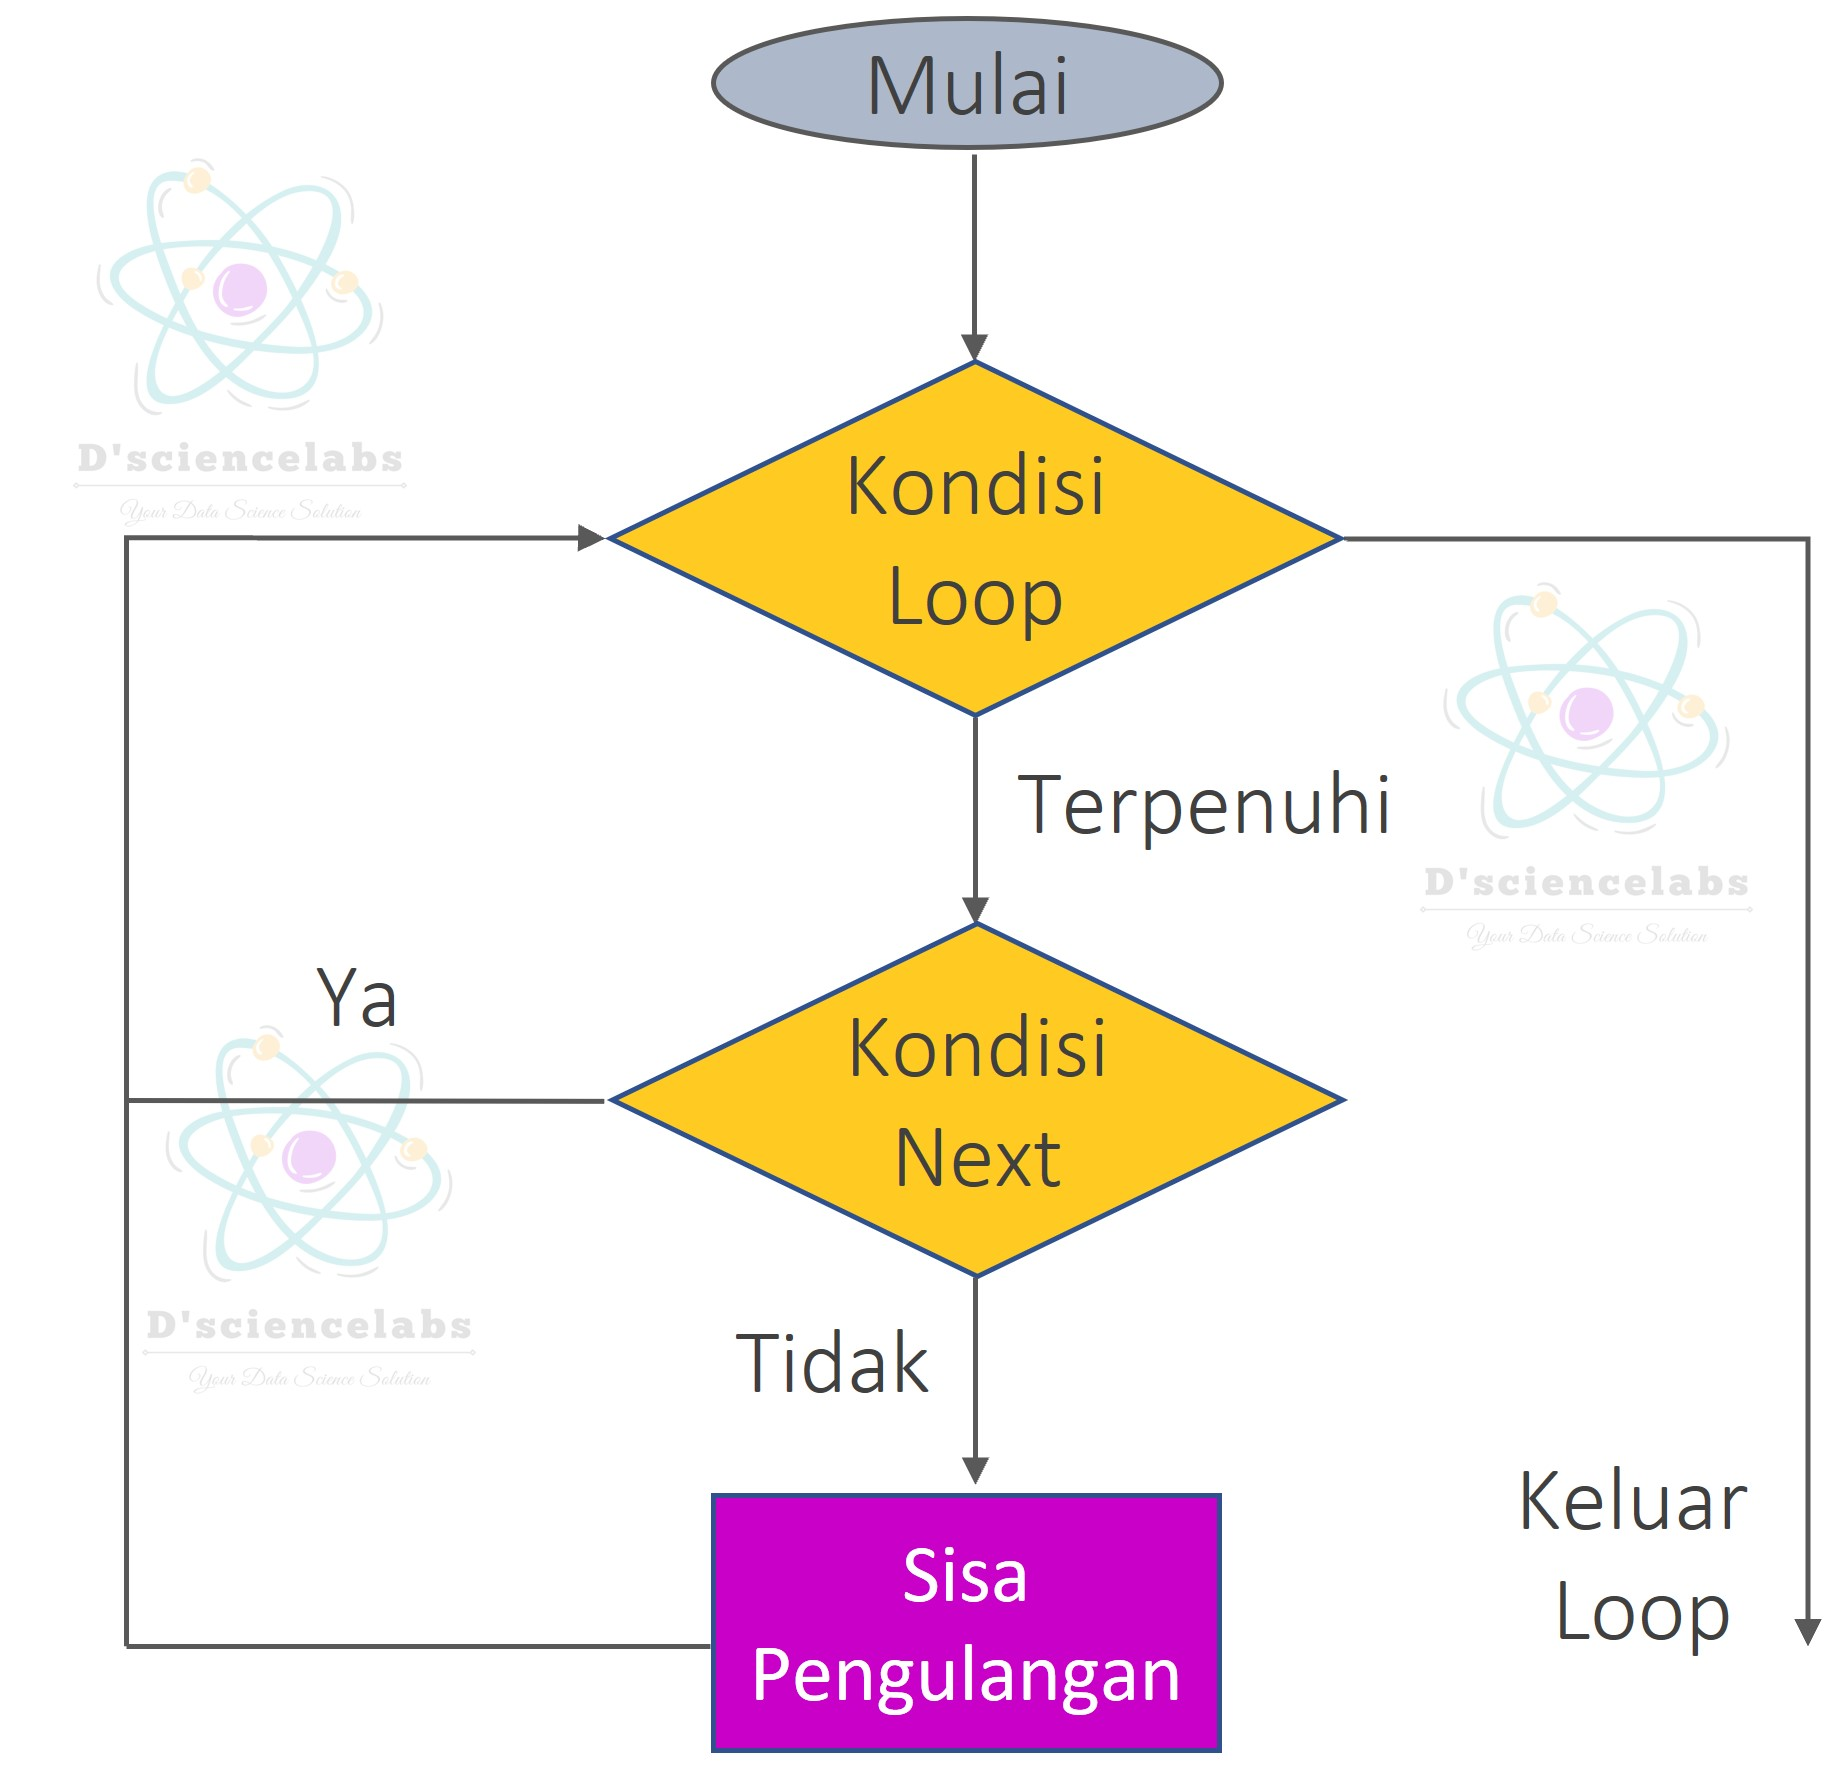
\includegraphics[width=1\linewidth]{./images/Bab6/next} 

}

\caption{Struktur Kontrol next}\label{fig:next}
\end{figure}

\begin{verbatim}
for pengulangan {
  if (kondisi){
  next
  }
  print(val)
}
\end{verbatim}

Gunakan pernyataan \texttt{next}, misalnya untuk memeriksa apakah nilainya sama dengan 5. Jika nilainya sama dengan 5, evaluasi saat ini berhenti (nilai tidak dicetak) tetapi perulangan berlanjut dengan iterasi berikutnya.

\begin{Shaded}
\begin{Highlighting}[]
\NormalTok{x }\OtherTok{\textless{}{-}} \DecValTok{1}\SpecialCharTok{:}\DecValTok{11}
 \ControlFlowTok{for}\NormalTok{ (val }\ControlFlowTok{in}\NormalTok{ x) \{}
 \ControlFlowTok{if}\NormalTok{ (val }\SpecialCharTok{==} \DecValTok{5}\NormalTok{)\{}
 \ControlFlowTok{next}
\NormalTok{ \}}
\FunctionTok{print}\NormalTok{(val)}
\NormalTok{\}}
\end{Highlighting}
\end{Shaded}

\begin{verbatim}
## [1] 1
## [1] 2
## [1] 3
## [1] 4
## [1] 6
## [1] 7
## [1] 8
## [1] 9
## [1] 10
## [1] 11
\end{verbatim}

\hypertarget{latihan-4}{%
\section{Latihan}\label{latihan-4}}

\begin{enumerate}
\def\labelenumi{\arabic{enumi}.}
\item
  Pernyataan Kondisional (if-else):
  Buatlah sebuah program yang memeriksa apakah suatu bilangan adalah positif, negatif, atau nol, dan mencetak pesan yang sesuai.
\item
  Pengulangan (for):
  Hitunglah jumlah dari semua bilangan bulat genap antara 1 dan 50 menggunakan loop for.
\item
  Pengulangan (while):
  Buatlah program yang meminta pengguna untuk menebak suatu angka acak antara 1 dan 100. Berikan petunjuk apakah angka yang ditebak terlalu besar atau terlalu kecil, dan berhenti ketika pengguna berhasil menebak angka tersebut.
\item
  Pernyataan Switch:
  Buatlah program yang mengonversi nama hari dalam bahasa Inggris menjadi nama hari dalam bahasa Indonesia menggunakan pernyataan switch.
\item
  Pengulangan dan Pernyataan Kondisional Gabungan:
  Hitunglah jumlah bilangan bulat positif yang dapat dibagi habis oleh 3 atau 5 di antara 1 dan 1000, lalu cetak hasilnya.
\item
  Nested Loop:
  Buatlah pola segitiga angka seperti berikut menggunakan nested loop:
\end{enumerate}

\begin{verbatim}
1
12
123
1234
12345
\end{verbatim}

\begin{enumerate}
\def\labelenumi{\arabic{enumi}.}
\setcounter{enumi}{6}
\item
  Penggunaan break:
  Buatlah sebuah program yang mencari bilangan prima pertama yang lebih dari 100.
\item
  Fungsi Rekursif:
  Buatlah fungsi rekursif untuk menghitung bilangan Fibonacci ke-n.
\end{enumerate}

\textbf{Catatan:} Kumpulkan hasil latihan anda, tidak boleh sama dengan teman mahasiwa lainnya.

\hypertarget{interface-data}{%
\chapter{Interface Data}\label{interface-data}}

Terhubung dengan data adalah hal paling mendasar dalam preses olah data (Data Science). Pada bagian ini akan dibahas bagaimana proses antarmuka data yang paling sederhana dengan menggunakan R. Secara garis besar R dapat membaca data dari file yang disimpan di dalam maupun luar direktorinya. Selain itu, sistem operasi R juga dapat menyimpan dan membaca data dalam berbagai format file seperti csv, excel, txt, rds, xml, json, dll.

\begin{figure}

{\centering 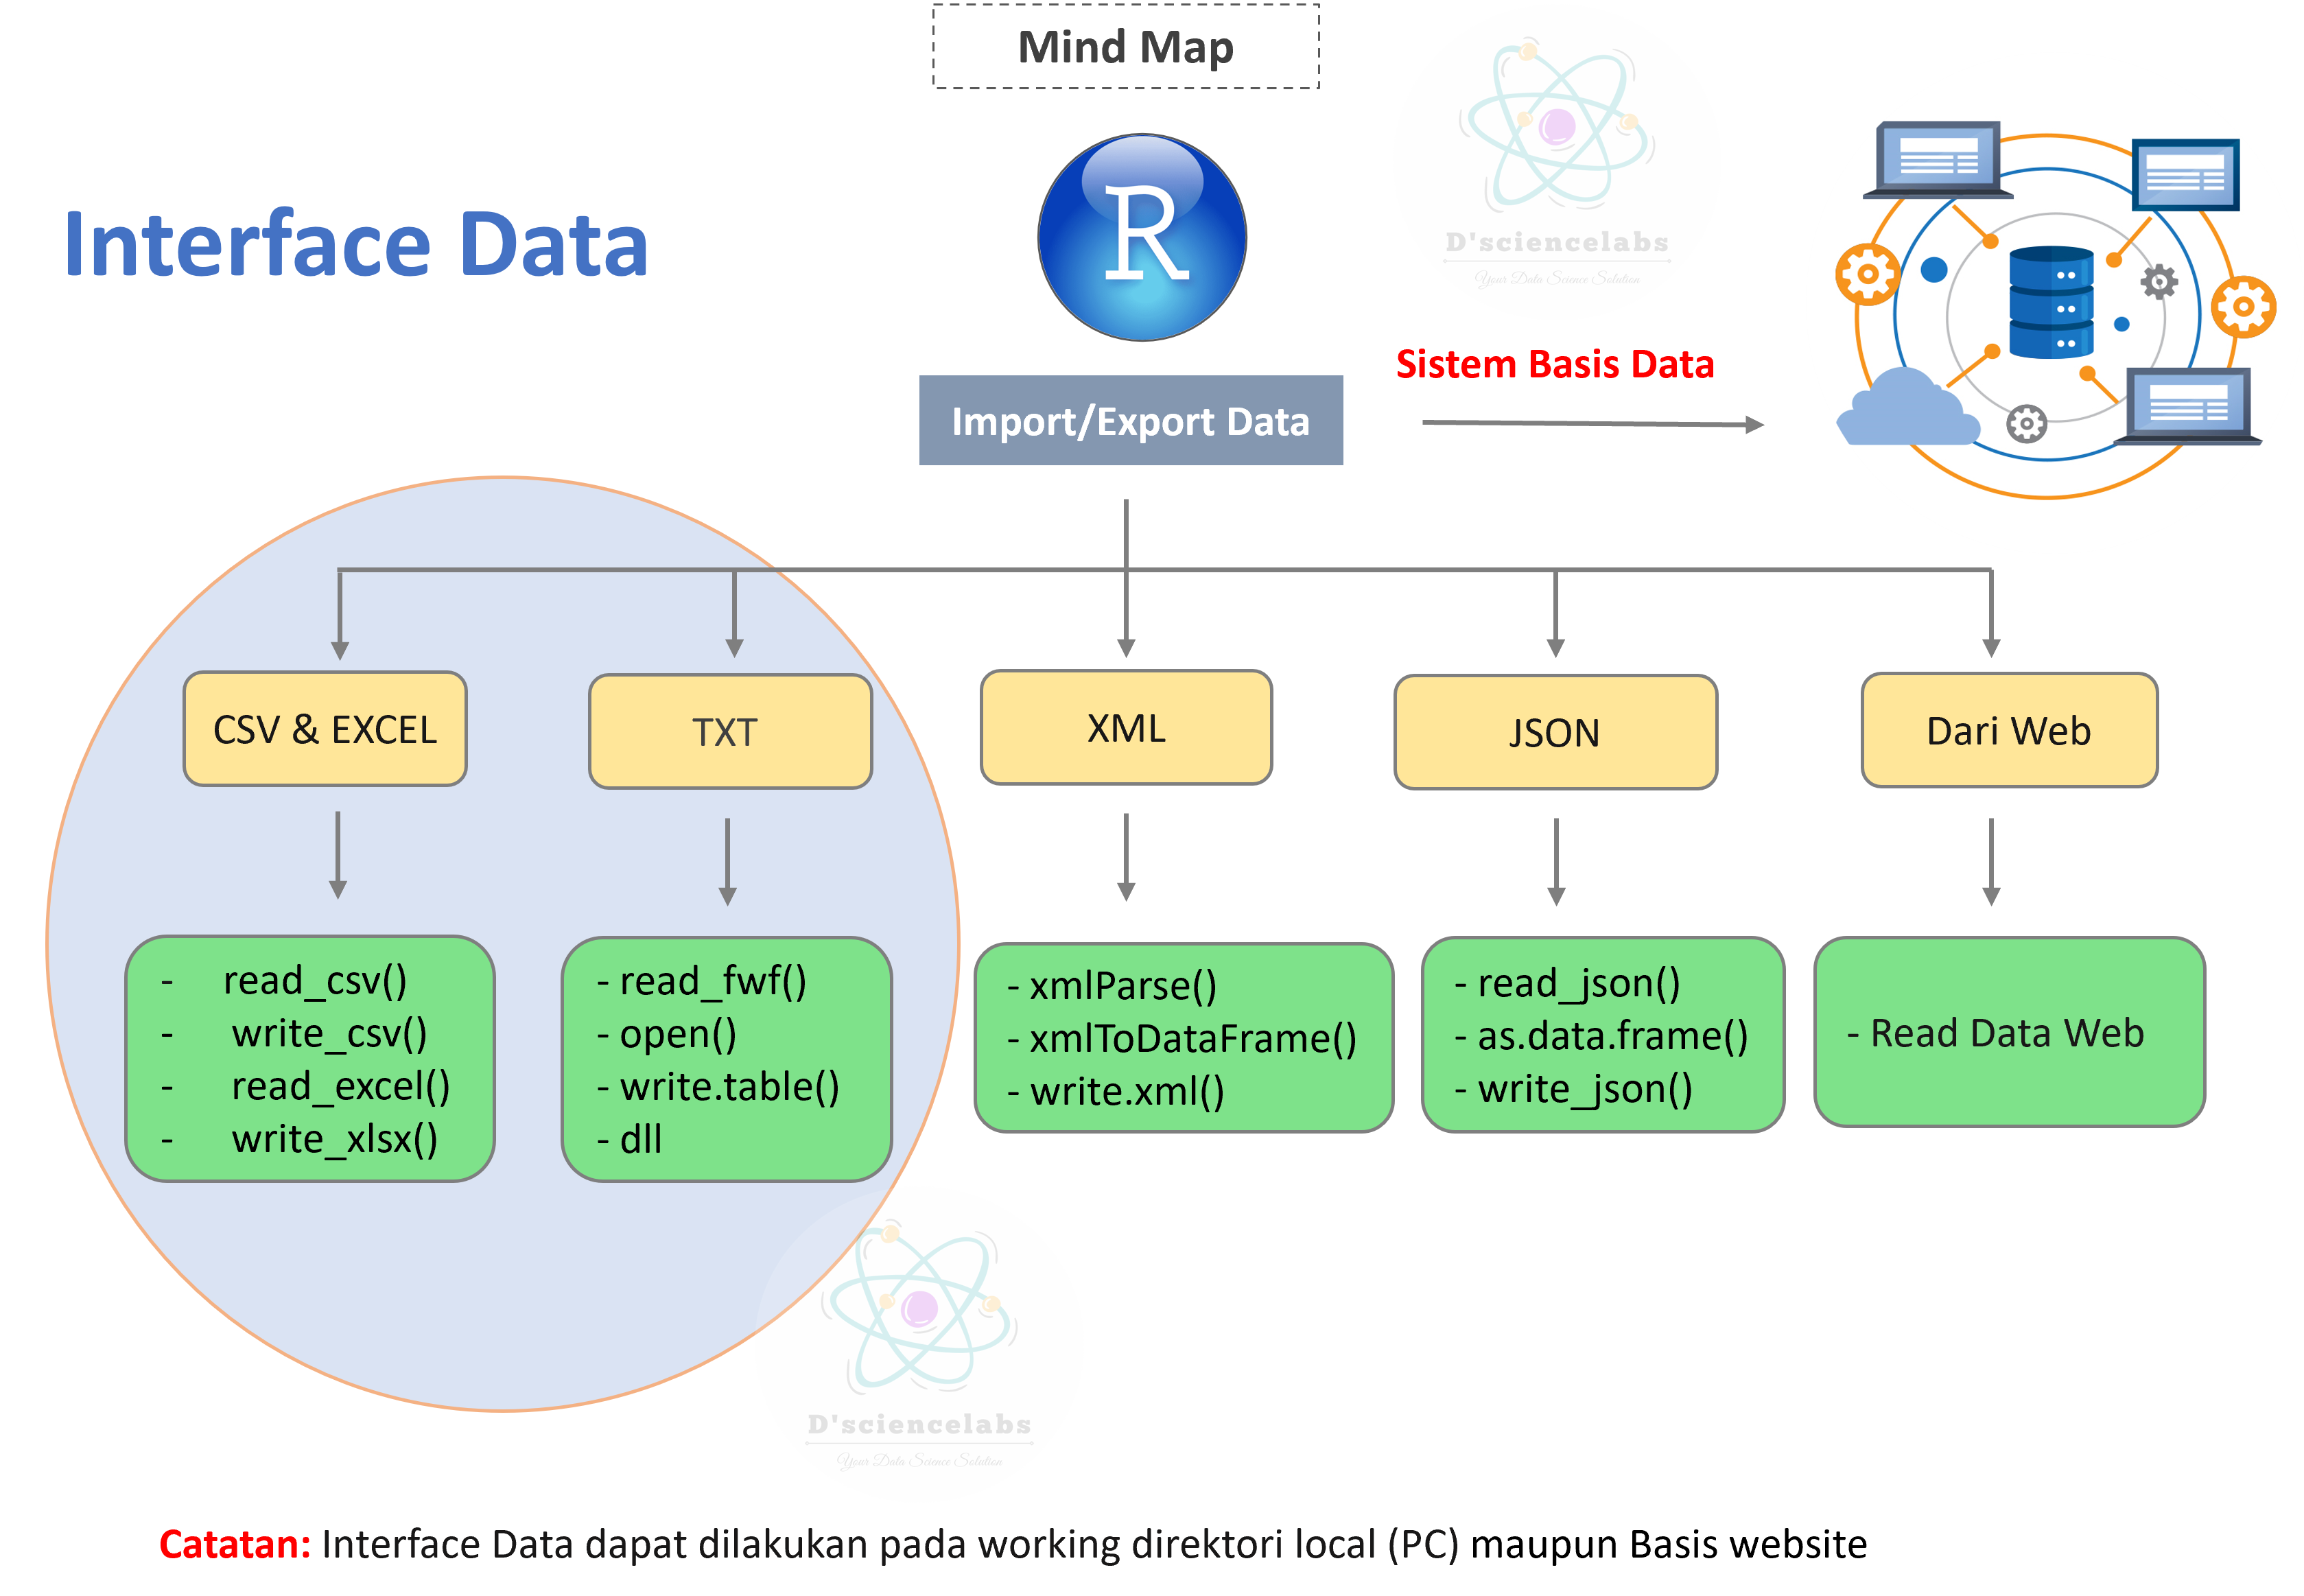
\includegraphics[width=1\linewidth]{./images/Bab7/Interface_Data} 

}

\caption{Interface Data}\label{fig:interface}
\end{figure}

\textbf{Catatan:} Data yang digunakan dalam pembelajaran ini, dapat download pada link berikut!

\begin{itemize}
\tightlist
\item
  \href{https://github.com/dsciencelabs/Algoritma_Pemrograman_R/blob/main/Data/Input/input1.csv}{input1.csv}
\item
  \href{https://github.com/dsciencelabs/Algoritma_Pemrograman_R/blob/main/Data/Input/input2.csv}{input2.csv}
\item
  \href{https://github.com/dsciencelabs/Algoritma_Pemrograman_R/blob/main/Data/Input/input3.xls}{input3.xls}
\item
  \href{https://github.com/dsciencelabs/Algoritma_Pemrograman_R/blob/main/Data/Input/input4.xlsx}{input4.xlsx}
\item
  \href{https://github.com/dsciencelabs/Algoritma_Pemrograman_R/blob/main/Data/Input/input5.txt}{input5.txt}
\item
  \href{https://github.com/dsciencelabs/Algoritma_Pemrograman_R/blob/main/Data/Input/input6.Rdmpd}{input6.Rdmpd}
\item
  \href{https://github.com/dsciencelabs/Algoritma_Pemrograman_R/blob/main/Data/Input/input7.rds}{input7.rds}
\item
  \href{https://github.com/dsciencelabs/Algoritma_Pemrograman_R/blob/main/Data/Input/input8.ascii}{input8.ascii}
\item
  \href{https://github.com/dsciencelabs/Algoritma_Pemrograman_R/blob/main/Data/Input/input9.xml}{input9.xml}
\item
  \href{https://github.com/dsciencelabs/Algoritma_Pemrograman_R/blob/main/Data/Input/input10.json}{input10.json}
\end{itemize}

\hypertarget{imporekspor-csv}{%
\section{Impor/Ekspor CSV}\label{imporekspor-csv}}

Terdapat beberapa cara yang dapat dilakukan untuk impor/expor data dengan R. Berikut ini, diperlihatkan 3 cara yang paling sering digunakan dalam proses antarmuka data.

\hypertarget{cara-1}{%
\subsection{Cara 1}\label{cara-1}}

Pertama-tama pastikan direktori kerja anda dalam koneksi yang benar, periksalah dengan menggunakan fungsi \texttt{getwd()}. Kemudian, anda dapat mengatur direktori kerja baru menggunakan fungsi \texttt{setwd()}.

\begin{Shaded}
\begin{Highlighting}[]
\FunctionTok{print}\NormalTok{(}\FunctionTok{getwd}\NormalTok{())                                   }\CommentTok{\# cetak direktori kerja R}
\FunctionTok{getwd}\NormalTok{()                                          }\CommentTok{\# cetak direktori kerja R}
\CommentTok{\#setwd("C:/Users/Bakti/Desktop/")                \# atur direktori (ini contoh)}
\CommentTok{\#setwd("C:\textbackslash{}\textbackslash{}Users\textbackslash{}\textbackslash{}Bakti\textbackslash{}\textbackslash{}Desktop\textbackslash{}\textbackslash{}")            \# atau dengan cara ini}
\end{Highlighting}
\end{Shaded}

Selanjutnya, proses impor data CSV dengan menggunakan fungsi \texttt{read.csv()}.

\begin{Shaded}
\begin{Highlighting}[]
\FunctionTok{setwd}\NormalTok{(}\FunctionTok{getwd}\NormalTok{())                                    }\CommentTok{\# setting direktori}
\NormalTok{df1 }\OtherTok{\textless{}{-}}\FunctionTok{read.csv}\NormalTok{(}\StringTok{"Data/Input/input1.csv"}\NormalTok{,}\AttributeTok{sep =} \StringTok{","}\NormalTok{) }\CommentTok{\# format pemisah koma }
\NormalTok{df2 }\OtherTok{\textless{}{-}}\FunctionTok{read.csv}\NormalTok{(}\StringTok{"Data/Input/input2.csv"}\NormalTok{,}\AttributeTok{sep =} \StringTok{";"}\NormalTok{) }\CommentTok{\# format pemisah titik koma}
\end{Highlighting}
\end{Shaded}

Jika anda ingin melakukan expor data (simpan) ke direktori yang diinginkan maka dapat dilakukan dengan menggunakan fungsi \texttt{write.csv()} untuk format data dengan pemisah koma \texttt{(",")} dan fungsi \texttt{write.csv2()} untuk format data dengan pemisah semicolon \texttt{(";")}.

\begin{Shaded}
\begin{Highlighting}[]
\FunctionTok{write.csv}\NormalTok{(df1,}\StringTok{"Data/Output/output1.csv"}\NormalTok{, }\AttributeTok{row.names =} \ConstantTok{FALSE}\NormalTok{)  }
\FunctionTok{write.csv2}\NormalTok{(df2,}\StringTok{"Data/Output/output2.csv"}\NormalTok{, }\AttributeTok{row.names =} \ConstantTok{FALSE}\NormalTok{)    }
\end{Highlighting}
\end{Shaded}

\hypertarget{cara-2}{%
\subsection{Cara 2}\label{cara-2}}

Bagi anda yang lebih menyukai koneksi direktori secara automatis, cara ini adalah pilihan yang yang lebih bijak dan praktis.

\begin{Shaded}
\begin{Highlighting}[]
\CommentTok{\# setting direktori}
\NormalTok{(WD }\OtherTok{\textless{}{-}} \FunctionTok{getwd}\NormalTok{())}
\ControlFlowTok{if}\NormalTok{ (}\SpecialCharTok{!}\FunctionTok{is.null}\NormalTok{(WD)) }\FunctionTok{setwd}\NormalTok{(WD)}
\end{Highlighting}
\end{Shaded}

\begin{Shaded}
\begin{Highlighting}[]
\CommentTok{\# impor data}
\NormalTok{df1 }\OtherTok{\textless{}{-}} \FunctionTok{read.csv}\NormalTok{(}\FunctionTok{file.path}\NormalTok{(WD, }\StringTok{\textquotesingle{}Data/Input\textquotesingle{}}\NormalTok{, }\StringTok{\textquotesingle{}input1.csv\textquotesingle{}}\NormalTok{))}
\NormalTok{df2 }\OtherTok{\textless{}{-}} \FunctionTok{read.csv}\NormalTok{(}\FunctionTok{file.path}\NormalTok{(WD, }\StringTok{\textquotesingle{}Data/Input\textquotesingle{}}\NormalTok{, }\StringTok{\textquotesingle{}input2.csv\textquotesingle{}}\NormalTok{))}

\CommentTok{\# ekspor data}
\FunctionTok{write.csv}\NormalTok{(df1, }\FunctionTok{file.path}\NormalTok{(WD, }\StringTok{\textquotesingle{}Data/Output\textquotesingle{}}\NormalTok{, }\StringTok{\textquotesingle{}output1.csv\textquotesingle{}}\NormalTok{),}\AttributeTok{row.names =} \ConstantTok{FALSE}\NormalTok{)}
\FunctionTok{write.csv}\NormalTok{(df2, }\FunctionTok{file.path}\NormalTok{(WD, }\StringTok{\textquotesingle{}Data/Output\textquotesingle{}}\NormalTok{, }\StringTok{\textquotesingle{}output2.csv\textquotesingle{}}\NormalTok{),}\AttributeTok{row.names =} \ConstantTok{FALSE}\NormalTok{)}
\end{Highlighting}
\end{Shaded}

\hypertarget{cara-3}{%
\subsection{Cara 3}\label{cara-3}}

Cara ini adalah langkah alternatif bagi anda yang lebih nyaman untuk memilih data yang tersimpan di komputer (PC) tanpa harus melakukan pengaturan direktori terlebih dahulu sebelum melakukan proses impor data.

\begin{Shaded}
\begin{Highlighting}[]
\NormalTok{df3 }\OtherTok{\textless{}{-}} \FunctionTok{read.csv}\NormalTok{(}\FunctionTok{file.choose}\NormalTok{())}
\end{Highlighting}
\end{Shaded}

\textbf{Catatan:} Proses impor/eskpor data selanjutnya akan dilakukan dengan cara 1 satu saja.

\hypertarget{imporekspor-excel}{%
\section{Impor/Ekspor Excel}\label{imporekspor-excel}}

Microsoft Excel adalah program spreadsheet yang paling banyak digunakan yang menyimpan data dalam format \texttt{.xls} atau \texttt{.xlsx}. R dapat membaca langsung dari file-file ini menggunakan paket \texttt{readxl}.

\begin{Shaded}
\begin{Highlighting}[]
\CommentTok{\# install.packages(c("readxl", "writexl"))       \# install \textasciigrave{}readxl \& writexl\textasciigrave{} }
\NormalTok{pacman}\SpecialCharTok{::}\FunctionTok{p\_load}\NormalTok{(readxl, writexl)                  }\CommentTok{\# load \textasciigrave{}readxl \& writexl\textasciigrave{}}

\CommentTok{\# impor data}
\NormalTok{df3}\OtherTok{\textless{}{-}}\FunctionTok{read\_excel}\NormalTok{(}\StringTok{"Data/Input/input3.xls"}\NormalTok{)         }\CommentTok{\# impor data xls (97{-}2003)}
\NormalTok{df4}\OtherTok{\textless{}{-}}\FunctionTok{read\_excel}\NormalTok{(}\StringTok{"Data/Input/input4.xlsx"}\NormalTok{,}\AttributeTok{sheet=}\DecValTok{1}\NormalTok{)}\CommentTok{\# impor data xlsx (2003{-}up)}

\CommentTok{\# ekspor data}
\FunctionTok{write\_xlsx}\NormalTok{(df3,}\StringTok{"Data/Output/output3.xls"}\NormalTok{) }
\FunctionTok{write\_xlsx}\NormalTok{(df4,}\StringTok{"Data/Output/output4.xlsx"}\NormalTok{)}
\end{Highlighting}
\end{Shaded}

\hypertarget{imporekspor-txt-and-rds}{%
\section{Impor/Ekspor TXT and RDS}\label{imporekspor-txt-and-rds}}

Format data paling umum yang sering digunakan untuk impor/ekspor data adalah file CSV dan XLSX. Namun, ukuran file CSV atau XLSX cendrung lebih besar dibanding format yang lainya seperti TXT atau file biner R (RDS). Sehingga, ini akan membutuhkan tambahan waktu pada saat anda melakukan impor/ekspor data. Tips, yang sangat saya rekomendasikan dalam hal ini adalah mengimpor dan ekspor data tersebut dengan format TXT atau binary.

\begin{Shaded}
\begin{Highlighting}[]
\CommentTok{\# impor data}
\NormalTok{df5 }\OtherTok{\textless{}{-}} \FunctionTok{read.table}\NormalTok{(}\StringTok{"Data/Input/input5.txt"}\NormalTok{)       }\CommentTok{\# format TXT (notepad)}
\NormalTok{df6 }\OtherTok{\textless{}{-}} \FunctionTok{source}\NormalTok{(}\StringTok{"Data/Input/input6.Rdmpd"}\NormalTok{)         }\CommentTok{\# format TXT (Rdmpd)}
\NormalTok{df7 }\OtherTok{\textless{}{-}} \FunctionTok{readRDS}\NormalTok{(}\StringTok{"Data/Input/input7.rds"}\NormalTok{)          }\CommentTok{\# format binary RDS }
\NormalTok{df8 }\OtherTok{\textless{}{-}} \FunctionTok{readRDS}\NormalTok{(}\StringTok{"Data/Input/input8.ascii"}\NormalTok{)        }\CommentTok{\# format binary ASCII }

\CommentTok{\# ekspor data}
\FunctionTok{write.table}\NormalTok{(df5,}\StringTok{"Data/Output/output5.txt"}\NormalTok{)                }
\FunctionTok{dump}\NormalTok{(}\StringTok{"df6"}\NormalTok{, }\StringTok{"Data/Output/output6.Rdmpd"}\NormalTok{)                    }
\FunctionTok{saveRDS}\NormalTok{(df7, }\StringTok{"Data/Output/output7.rds"}\NormalTok{)                      }
\FunctionTok{saveRDS}\NormalTok{(df8, }\StringTok{"Data/Output/output8.ascii"}\NormalTok{, }\AttributeTok{ascii=}\ConstantTok{TRUE}\NormalTok{)             }
\end{Highlighting}
\end{Shaded}

\textbf{Catatan:} Format binary sangat lazim digunakan untuk meringkas file yang berukuran besar, terutama saat menggunakan sistem kontrol (API) seperti halnya \href{https://git-scm.com/}{Git}.

\hypertarget{imporekspor-xml}{%
\section{Impor/Ekspor XML}\label{imporekspor-xml}}

XML adalah kumpulan berbagi format file dan data di World Wide Web, intranet, dan di tempat lain menggunakan teks ASCII standar. XML adalah singkatan dari eXtensible Markup Language. Untuk penjelasan lebih lengkap silahkan kunjungi

Sebenarnya XML sangat mirip dengan HTML, diman sintak-sintaknya berisi markup. Tetapi, perlu dicatat bahwa XML tidak sama dalam hal tag markup HTML yang menjelaskan laman struktur datanya terdapat dalam file tersebut. Silahkah perhatikan video penjelasan mengenai HTML;

Selanjutnya, mari kita lakukan impor/ekspor data dengan format XML.

\begin{Shaded}
\begin{Highlighting}[]
\FunctionTok{library}\NormalTok{(}\StringTok{"XML"}\NormalTok{)                                   }\CommentTok{\# load paket XML }
\FunctionTok{library}\NormalTok{(}\StringTok{"kulife"}\NormalTok{)                                }\CommentTok{\# load paket kulife}
\FunctionTok{library}\NormalTok{(}\StringTok{"methods"}\NormalTok{)                               }\CommentTok{\# paket kondisional}

\NormalTok{df9 }\OtherTok{\textless{}{-}} \FunctionTok{xmlParse}\NormalTok{(}\StringTok{"Data/Input/input9.xml"}\NormalTok{)         }\CommentTok{\# impor data XML}
\NormalTok{xml\_df }\OtherTok{\textless{}{-}} \FunctionTok{xmlToDataFrame}\NormalTok{(df9)                    }\CommentTok{\# konversi ke Dataframe}
\FunctionTok{write.xml}\NormalTok{(xml\_df, }\StringTok{"Data/Output/output9.xml"}\NormalTok{)     }\CommentTok{\# ekspor data XML}
\end{Highlighting}
\end{Shaded}

\hypertarget{imporekspor-json}{%
\section{Impor/Ekspor JSON}\label{imporekspor-json}}

File JSON menyimpan data sebagai teks dalam format yang dapat dibaca manusia. Json adalah singkatan dari JavaScript Object Notation. R dapat membaca file JSON menggunakan paket \texttt{jsonlite}. Selengkapnya tentang JSON

\begin{Shaded}
\begin{Highlighting}[]
\FunctionTok{library}\NormalTok{(}\StringTok{"jsonlite"}\NormalTok{)                              }\CommentTok{\# load paket JSON}

\NormalTok{df10 }\OtherTok{\textless{}{-}}\FunctionTok{fromJSON}\NormalTok{(}\StringTok{"Data/Input/input10.json"}\NormalTok{)       }\CommentTok{\# impor data}
\NormalTok{json\_df }\OtherTok{\textless{}{-}} \FunctionTok{as.data.frame}\NormalTok{(df10)                   }\CommentTok{\# konversi ke Dataframe}
\FunctionTok{write\_json}\NormalTok{(json\_df, }\StringTok{"Data/Output/output10.json"}\NormalTok{) }\CommentTok{\# ekspor data JSON}
\end{Highlighting}
\end{Shaded}

\hypertarget{impor-data-dari-web}{%
\section{Impor Data dari Web}\label{impor-data-dari-web}}

Ada banyak website menyediakan data untuk dikonsumsi oleh penggunanya. Dengan menggunakan program R, kita dapat mengekstrak data spesifik dari situs web tersebut secara terprogram. Di bagian ini, saya memberikan contoh cara mengimpor data dari repositori GitHub, tetapi Anda dapat melakukan hal yang sama ke situs web atau repositori lain.

\hypertarget{csv}{%
\subsection{CSV:}\label{csv}}

\begin{Shaded}
\begin{Highlighting}[]
\NormalTok{web\_csv }\OtherTok{\textless{}{-}} \FunctionTok{read.csv}\NormalTok{(}\StringTok{"https://raw.githubusercontent.com/dsciencelabs/Algoritma\_Pemrograman\_R/main/Data/Input/input1.csv"}\NormalTok{)}
\end{Highlighting}
\end{Shaded}

\hypertarget{xlsx}{%
\subsection{XLSX:}\label{xlsx}}

\begin{Shaded}
\begin{Highlighting}[]
\FunctionTok{library}\NormalTok{(rio)                          }\CommentTok{\# impor data dari github}
\FunctionTok{install\_formats}\NormalTok{()                     }\CommentTok{\# periksa auto paket yg disarankan}
\NormalTok{web\_xlsx }\OtherTok{\textless{}{-}}\NormalTok{rio}\SpecialCharTok{::}\FunctionTok{import}\NormalTok{(}\StringTok{"https://github.com/dsciencelabs/Algoritma\_Pemrograman\_R/raw/main/Data/Input/input4.xlsx"}\NormalTok{)}
\end{Highlighting}
\end{Shaded}

\hypertarget{basis-data-r}{%
\section{Basis Data R}\label{basis-data-r}}

Sistem basis data adalah data relasional yang disimpan dalam format yang dinormalisasi. Jadi, untuk melakukan komputasi statistik kita akan membutuhkan query SQL yang sangat canggih dan kompleks. Tetapi R dapat terhubung dengan mudah ke banyak database relasional seperti MySql, Oracle, SQL Server, dll. Selanjutnya biasanya, kita akan mengubah basis data tersebut menjadi bingkai data (data frame). Setelah data tersedia di lingkungan R, kemudian dimanipulasi atau dilakukan analisis lebih lanjut.

\textbf{Catatan:} Kita akan mempelajari bagian ini di bagian khusus yang disebut ``Sistem Basis Data dengan R'' semester berikutnya.

\hypertarget{menambang-data-web}{%
\section{Menambang Data Web}\label{menambang-data-web}}

Pengikisan data dari web (Webscraping Data) adalah proses menggunakan bot untuk mengekstrak konten dan data dari situs web. Tidak seperti screen scraping, yang hanya menyalin piksel yang ditampilkan di layar, web scraping mengekstrak kode HTML yang mendasarinya yang pada dasarnya disimpan dalam database. Pengikisan data ini dapat mereplikasi seluruh konten dari berbagai situs web yang target.

\textbf{Catatan:} Kita akan mempelajari bagian ini di bagian khusus yang disebut ``Ilmu Data Terapan''.

\hypertarget{latihan-5}{%
\section{Latihan}\label{latihan-5}}

Buatlah tutorial Baca dan Simpan data dengan mengikuti materi yang sudah dipelajari diatas. Lengkapi dengan Gambar dan penjelasan setiap prosesnya.

\textbf{Catatan:} Kumpulkan hasil latihan anda, tidak boleh sama dengan teman mahasiwa lainnya.

\hypertarget{manipulasi-data}{%
\chapter{Manipulasi Data}\label{manipulasi-data}}

Salah satu keterampilan paling mendasar yang harus dimiliki seorang Data Scientist adalah memanipulasi data. Untuk menjadi seseorang yang sangat efektif, Anda harus ahli dalam memanipulasi data penting. Hal ini perlu diperhatikan karena sebagian besar pekerjaan Anda akan melibatkan \href{https://www.forbes.com/sites/gilpress/2016/03/23/data-preparation-most-time-consuming-least-enjoyable-data-science-task-survey-says/\#4b432fa66f63}{pengambilan dan pembersihan data}.

Data Scientist menghabiskan 60\% waktunya untuk membersihkan dan mengatur data. Di urutan kedua, 19\% waktunya untuk mengumpulkan dataset, yang berarti Data Scientist menghabiskan sekitar 80\% waktunya untuk menyiapkan dan mengelola data untuk analisis.

Pada bagian ini, Anda akan mempelajari bagaimana memanipulasi data dengan mudah menggunakan R. Kita akan membahas fungsi-fungsi manipulasi data mendasar yang sebagian besar akan Anda gunakan untuk memanipulasi data Anda.

\begin{itemize}
\tightlist
\item
  \texttt{read\_csv()} Mengimpor data (Anda bisa menggunakan fungsi lainnya)
\item
  \texttt{str()} Struktur Data
\item
  \texttt{apply()} Untuk mengecek dan mengganti data yang hilang.
\item
  \texttt{select()} Memilih kolom yang akan disertakan.
\item
  \texttt{filter()} Memilih subset yang ada di dalam data.
\item
  \texttt{arrange()} Mengurutkan data, berdasarkan ukuran dari variabel kontinu, berdasarkan tanggal, atau menurut abjad.
\item
  \texttt{rename()} Mengganti nama kolom.
\item
  \texttt{mutate()} Membuat kolom baru di dalam data, atau mengganti kolom yang sudah ada.
\item
  \texttt{bind\_rows()} Menggabungkan dua data frame menjadi satu, menggabungkan data dari kolom-kolom dengan nama yang sama.
\item
  \texttt{group\_by()} Mengelompokkan data berdasarkan variabel kategorikal.
\item
  \texttt{summarize()} Meringkas, atau mengagregat (untuk setiap kelompok jika mengikuti \texttt{group\_by}). Sering digunakan bersama fungsi sebagai berikut:

  \begin{itemize}
  \tightlist
  \item
    \texttt{mean()} Menghitung rata-rata.
  \item
    \texttt{median()} Menghitung median.
  \item
    \texttt{max()} Mencari nilai maksimum.
  \item
    \texttt{min()} Mencari nilai minimum.
  \item
    \texttt{sum()} Menambahkan semua nilai secara bersamaan.
  \item
    \texttt{n()} Menghitung jumlah record.
  \end{itemize}
\end{itemize}

Saya menyarankan Anda untuk menginstal package \href{https://www.tidyverse.org/packages/}{\texttt{tidyverse}}. Karena inti dari \texttt{tidyverse} mencakup packages yang cendrung Anda gunakan dalam analisis data sehari-hari.

\begin{Shaded}
\begin{Highlighting}[]
\FunctionTok{install.packages}\NormalTok{(}\StringTok{"tidyverse"}\NormalTok{)}
\end{Highlighting}
\end{Shaded}

Kita sebagian besar akan bekerja dengan dua package yang sangat berguna yang dikembangkan oleh \href{http://hadley.nz/}{Hardley Wickham}, kepala scientist di RStudio:

\begin{itemize}
\tightlist
\item
  \href{https://readr.tidyverse.org/}{\texttt{readr}} Untuk membaca dan menulis CSV dan file teks lainnya.
\item
  \href{https://dplyr.tidyverse.org/}{\texttt{dplyr}} Untuk memproses dan memanipulasi data.
\end{itemize}

\hypertarget{impor-data}{%
\section{Impor Data}\label{impor-data}}

\href{https://raw.githubusercontent.com/dsciencelabs/Algoritma_Pemrograman_R/main/Data/pfizer.csv}{Data} yang akan kita gunakan pada bagian ini adalah \texttt{pfizer.csv} dan \texttt{fda.csv}, silakan unduh dan tempatkan di desktop Anda. Sebagai opsional, Anda dapat memuat data ke sesi R saat ini dengan memilih \texttt{Import\ Dataset\textgreater{}From\ Teks\ File...} di tab Environment. Tapi, dalam hal ini kita akan menggunakan fungsi \texttt{read\_csv()} dari package \texttt{readr}. Salinlah kode berikut ke skrip Anda dan jalankan:

\begin{Shaded}
\begin{Highlighting}[]
\FunctionTok{suppressPackageStartupMessages}\NormalTok{(}\FunctionTok{library}\NormalTok{(tidyverse))}\CommentTok{\# memuat tidyverse}
\CommentTok{\#setwd("C:/Users/Bakti/Desktop/")                 \# ingatlah untuk mengatur working directory Anda}
\NormalTok{pfizer }\OtherTok{\textless{}{-}} \FunctionTok{read\_csv}\NormalTok{(}\StringTok{"Data/pfizer.csv"}\NormalTok{)             }\CommentTok{\# memuat data \textasciigrave{}pfizer\textasciigrave{} }
\end{Highlighting}
\end{Shaded}

\begin{Shaded}
\begin{Highlighting}[]
\NormalTok{fda }\OtherTok{\textless{}{-}} \FunctionTok{read\_csv}\NormalTok{(}\StringTok{"Data/fda.csv"}\NormalTok{)}
\end{Highlighting}
\end{Shaded}

\hypertarget{struktur-data-1}{%
\section{Struktur Data}\label{struktur-data-1}}

Perhatikan bahwa Anda akan membutuhkan pemahaman yang kuat mengenai tipe-tipe data mendasar dan struktur data dan bagaimana cara mengoprasikannya. Fungsi \texttt{str()} akan memberi tahu lebih banyak mengenai kolom dalam data Anda, termasuk tipe datanya. Salinlah kode berikut ke skrip Anda dan jalankan:

\begin{Shaded}
\begin{Highlighting}[]
\FunctionTok{str}\NormalTok{(pfizer)                                       }\CommentTok{\# melihat struktur dari data \textasciigrave{}pfizer\textasciigrave{}}
\FunctionTok{str}\NormalTok{(fda)                                          }\CommentTok{\# melihat struktur dari data \textasciigrave{}fda\textasciigrave{}}
\end{Highlighting}
\end{Shaded}

Sangat penting untuk dipahami karena ini adalah objek yang akan Anda manipulasi di R setiap saat. Jika Anda perlu mengubah tipe data untuk kolom apa pun, gunakan fungsi-fungsi di bawah ini:

\begin{itemize}
\tightlist
\item
  \texttt{as.character()} mengubah ke teks string.
\item
  \texttt{as.numeric()} mengubah ke angka.
\item
  \texttt{as.factor()} mengubah ke variabel kategorikal.
\item
  \texttt{as.integer()} mengubah ke bilangan bulat.
\item
  \texttt{as.Date()} mengubah ke tanggal.
\item
  \texttt{as.POSIXct()} mengubah ke tanggal dan waktu penuh.
\end{itemize}

Misalnya, tambahkan kode berikut ke skrip Anda untuk mengubah total konversi dalam data \texttt{pfizer} ke variabel numerik (yang memungkinkannya menyimpan nilai desimal, jika ada).

\begin{Shaded}
\begin{Highlighting}[]
\NormalTok{pfizer}\SpecialCharTok{$}\NormalTok{total }\OtherTok{\textless{}{-}} \FunctionTok{as.numeric}\NormalTok{(pfizer}\SpecialCharTok{$}\NormalTok{total)          }\CommentTok{\# konversi total ke variabel numerik}
\FunctionTok{str}\NormalTok{(pfizer}\SpecialCharTok{$}\NormalTok{total)                                 }\CommentTok{\# mari periksa struktur datanya lagi}
\end{Highlighting}
\end{Shaded}

\hypertarget{missing-value}{%
\section{Missing Value}\label{missing-value}}

Tidak seperti pemrograman biasa, ketika bekerja dengan data sesungguhnya, Anda mungkin menemukan \textbf{nilai yang hilang:} pengukuran yang tidak terekam/tersimpan/dll. R memiliki mekanisme yang cukup canggih untuk menangani nilai-nilai yang hilang. Ini membedakan antara jenis berikut:

\begin{itemize}
\tightlist
\item
  \texttt{NA} : Not Available (Nilai NA juga memiliki kelas, ada bilangan bulat NA, karakter NA, dll).
\item
  \texttt{NaN} : Not a Number (Nilai NaN juga merupakan NA tetapi NA bukan merupakan NaN)
\end{itemize}

Temukan nilai yang hilang di kolom dataframe \texttt{pfizer}

\begin{Shaded}
\begin{Highlighting}[]
\FunctionTok{is.na}\NormalTok{(pfizer)                                     }\CommentTok{\# cara untuk mengecek NA}
\FunctionTok{sum}\NormalTok{(}\FunctionTok{is.na}\NormalTok{(pfizer))                                }\CommentTok{\# menghitung jumlah NA}
\FunctionTok{apply}\NormalTok{(}\FunctionTok{is.na}\NormalTok{(pfizer),}\DecValTok{2}\NormalTok{, which)                     }\CommentTok{\# indeks NA (hanya df)}
\FunctionTok{which}\NormalTok{(}\FunctionTok{complete.cases}\NormalTok{(pfizer))                     }\CommentTok{\# mengidentifikasi nilai lengkap yang diamati}
\end{Highlighting}
\end{Shaded}

Mekanisme yang lebih umum adalah menghapusnya secara manual:

\begin{Shaded}
\begin{Highlighting}[]
\NormalTok{clean.vector}\OtherTok{\textless{}{-}} \FunctionTok{na.omit}\NormalTok{(pfizer}\SpecialCharTok{$}\NormalTok{first\_name)         }\CommentTok{\# bersihkan/hapus NA di vektor}
\NormalTok{clean.df }\OtherTok{\textless{}{-}} \FunctionTok{na.omit}\NormalTok{(pfizer)                       }\CommentTok{\# berishkan/hapus NA di dataframe}
\FunctionTok{apply}\NormalTok{(}\FunctionTok{is.na}\NormalTok{(clean.df),}\DecValTok{2}\NormalTok{, which)                   }\CommentTok{\# pastikan jika ada nilai yang hilang}
\end{Highlighting}
\end{Shaded}

\hypertarget{mengganti-nilai-yang-hilang}{%
\section{Mengganti Nilai yang Hilang}\label{mengganti-nilai-yang-hilang}}

Kita juga dapat mengganti nilai yang hilang dengan rata-rata (median). Praktik yang baik adalah dengan membuat dua variabel terpisah untuk mean. Setelah dibuat, kita dapat mengganti nilai yang hilang dengan variabel yang baru dibentuk. Mari unggah dan memeriksa data yang hilang.

\begin{Shaded}
\begin{Highlighting}[]
\NormalTok{PATH }\OtherTok{\textless{}{-}} \StringTok{"https://raw.githubusercontent.com/dsciencelabs/Algoritma\_Pemrograman\_R/main/Data/Missing\_Values.csv"}
\NormalTok{titanic }\OtherTok{\textless{}{-}} \FunctionTok{read.csv}\NormalTok{(PATH, }\AttributeTok{sep =} \StringTok{","}\NormalTok{)}
\NormalTok{list\_na }\OtherTok{\textless{}{-}} \FunctionTok{colnames}\NormalTok{(titanic)[ }\FunctionTok{apply}\NormalTok{(titanic, }\DecValTok{2}\NormalTok{, anyNA) ]}
\NormalTok{list\_na}
\end{Highlighting}
\end{Shaded}

Dalam hal ini, kita tidak menghapus semua nilai yang hilang, tetapi kita menggunakan metode \texttt{apply()} untuk menghitung rata-rata kolom dengan \texttt{NA}. Pertama, kita perlu menghitung rata-rata dengan argumen \texttt{na.rm\ =\ TRUE}. Argumen ini wajib karena kolom memiliki data yang hilang dan ini memberi tahu R untuk mengabaikannya.

\begin{Shaded}
\begin{Highlighting}[]
\NormalTok{average\_missing }\OtherTok{\textless{}{-}} \FunctionTok{apply}\NormalTok{(titanic[,}\FunctionTok{colnames}\NormalTok{(titanic) }\SpecialCharTok{\%in\%}\NormalTok{ list\_na],}
                         \DecValTok{2}\NormalTok{,}
\NormalTok{                         mean,}
                         \AttributeTok{na.rm =}  \ConstantTok{TRUE}\NormalTok{)}
\NormalTok{average\_missing}
\end{Highlighting}
\end{Shaded}

\textbf{Penjelasan Kode:} Terdapat 4 argumen di metode apply yang kita jalankan.

\begin{itemize}
\tightlist
\item
  \texttt{df} titanic{[},colnames(titanic) \%in\% list\_na{]}. Kode ini akan mengembalikan nama kolom dari objek list\_na (mis. ``age'' dan ``fare'').
\item
  \texttt{2} Menghitung fungsi pada kolom.
\item
  \texttt{mean} Menghitung rata-rata.
\item
  \texttt{na.rm\ =\ TRUE} Menolak nilai yang hilang.
\end{itemize}

Selanjutnya, kita dapat mengganti nilai-nilai \texttt{NA}. Fungsi mutate dari library \texttt{dplyr} berguna untuk membuat variabel baru. Kita tidak perlu mengubah kolom asli, jadi kita dapat membuat sebuah variabel baru tanpa \texttt{NA}. Fungsi mutate mudah digunakan, kita hanya perlu memilih nama variabel dan menentukan bagaimana cara membuat variabel tersebut. Berikut ini kode lengkapnya:

\begin{Shaded}
\begin{Highlighting}[]
\FunctionTok{library}\NormalTok{(dplyr)}
\NormalTok{titanic\_replace }\OtherTok{\textless{}{-}}\NormalTok{ titanic }\SpecialCharTok{\%\textgreater{}\%}
\FunctionTok{mutate}\NormalTok{(}\AttributeTok{age  =} \FunctionTok{ifelse}\NormalTok{(}\FunctionTok{is.na}\NormalTok{(Age), average\_missing[}\DecValTok{1}\NormalTok{], Age),}
\AttributeTok{fare =} \FunctionTok{ifelse}\NormalTok{(}\FunctionTok{is.na}\NormalTok{(Fare), average\_missing[}\DecValTok{2}\NormalTok{], Fare))}
\FunctionTok{sum}\NormalTok{(}\FunctionTok{is.na}\NormalTok{(titanic\_replace}\SpecialCharTok{$}\NormalTok{Age))}
\FunctionTok{sum}\NormalTok{(}\FunctionTok{is.na}\NormalTok{(titanic\_replace}\SpecialCharTok{$}\NormalTok{Fare))}
\end{Highlighting}
\end{Shaded}

Kolom usia asli memiliki 86 nilai yang hilang sementara variabel yang baru dibuat telah mengganti nilai yang hilang dengan rata-rata usia variabel. Anda dapat mencoba sendiri mengganti penelitian yang hilang dengan nilai median juga.

\hypertarget{memilih-data}{%
\section{Memilih Data}\label{memilih-data}}

Pada bagian ini, Anda akan mempelajari bagaimana cara memilih atau mengelompokkan kolom dataframe berdasarkan nama dan posisi menggunakan fungsi R yaitu \texttt{select()} dalam package \href{https://dplyr.tidyverse.org/reference/summarise.html}{\texttt{dplyr}}. Anda akan belajar cara menggunakan fungsi berikut ini:

\begin{itemize}
\tightlist
\item
  \texttt{pull()} mengekstrak nilai kolom sebagai sebuah vektor. Kolom bunga dapat ditentukan berdasarkan nama atau indeks.
\item
  \texttt{select()} mengekstrak satu atau beberapa kolom sebagai tabel data. Fungsi ini juga dapat menghapus kolom dari data frame.
\item
  \texttt{select\_if()} Memilih kolom berdasarkan kondisi tertentu. Seseorang dapat menggunakan fungsi ini, misalnya untuk memilih kolom jika numerik.
\item
  \textbf{Fungsi Pembantu:} \texttt{starts\_with()}, \texttt{ends\_with()}, \texttt{contains()}, \texttt{matches()}: Pilihlah kolom/variabel berdasarkan namanya.
\end{itemize}

\begin{Shaded}
\begin{Highlighting}[]
\FunctionTok{library}\NormalTok{(tidyverse)                                }\CommentTok{\# muat \textasciigrave{}tidyverse\textasciigrave{}, yang termasuk dalam \textasciigrave{}dplyr\textasciigrave{}}
\NormalTok{pfizer }\SpecialCharTok{\%\textgreater{}\%} \FunctionTok{pull}\NormalTok{(state) }\SpecialCharTok{\%\textgreater{}\%} \FunctionTok{head}\NormalTok{()                 }\CommentTok{\# ekstrak nilai kolom \textasciigrave{}state\textasciigrave{} sebagai vektor}
\NormalTok{pfizer }\SpecialCharTok{\%\textgreater{}\%} \FunctionTok{select}\NormalTok{(}\DecValTok{1}\SpecialCharTok{:}\DecValTok{3}\NormalTok{)                            }\CommentTok{\# memilih kolom 1 sampai 3}
\NormalTok{pfizer }\SpecialCharTok{\%\textgreater{}\%} \FunctionTok{select}\NormalTok{(}\DecValTok{1}\NormalTok{,}\DecValTok{3}\NormalTok{)                            }\CommentTok{\# memilih kolom 1 dan 3, tidak termasuk 2}
\NormalTok{pfizer }\SpecialCharTok{\%\textgreater{}\%} \FunctionTok{select}\NormalTok{(state}\SpecialCharTok{:}\NormalTok{total)                    }\CommentTok{\# memilih semua kolom dari \textasciigrave{}state\textasciigrave{} sampai \textasciigrave{}total\textasciigrave{}}
\NormalTok{pfizer }\SpecialCharTok{\%\textgreater{}\%} \FunctionTok{select}\NormalTok{(state,total)                    }\CommentTok{\# memilih kolom berdasarkan nama variabel}
\NormalTok{pfizer }\SpecialCharTok{\%\textgreater{}\%} \FunctionTok{select\_if}\NormalTok{(is.numeric)                  }\CommentTok{\# hanya memilih kolom numerik}
\NormalTok{pfizer }\SpecialCharTok{\%\textgreater{}\%} \FunctionTok{select\_if}\NormalTok{(is.character)                }\CommentTok{\# hanya memilih kolom karakter}
\NormalTok{pfizer }\SpecialCharTok{\%\textgreater{}\%} \FunctionTok{select}\NormalTok{(}\FunctionTok{starts\_with}\NormalTok{(}\StringTok{"first"}\NormalTok{))           }\CommentTok{\# hanya memilih kolom yang dimulai dengan \textasciigrave{}first\textasciigrave{}}
\NormalTok{pfizer }\SpecialCharTok{\%\textgreater{}\%} \FunctionTok{select}\NormalTok{(}\FunctionTok{ends\_with}\NormalTok{(}\StringTok{"name"}\NormalTok{))              }\CommentTok{\# hanya memilih kolom yang diakhiri dengan \textasciigrave{}name\textasciigrave{}}
\NormalTok{pfizer }\SpecialCharTok{\%\textgreater{}\%} \FunctionTok{select}\NormalTok{(}\FunctionTok{contains}\NormalTok{(}\StringTok{"rst"}\NormalTok{))                }\CommentTok{\# memilih kolom yang namanya mengandung \textasciigrave{}rst\textasciigrave{}}
\NormalTok{pfizer }\SpecialCharTok{\%\textgreater{}\%} \FunctionTok{select}\NormalTok{(}\FunctionTok{matches}\NormalTok{(}\StringTok{"\_"}\NormalTok{))                   }\CommentTok{\# memilih kolom yang namanya cocok dengan reguler}
\NormalTok{pfizer }\SpecialCharTok{\%\textgreater{}\%} \FunctionTok{select}\NormalTok{(}\SpecialCharTok{{-}}\NormalTok{(state}\SpecialCharTok{:}\NormalTok{total))                 }\CommentTok{\# menghapus semua kolom dari \textasciigrave{}state\textasciigrave{} sampai \textasciigrave{}total\textasciigrave{}}
\NormalTok{pfizer }\SpecialCharTok{\%\textgreater{}\%} \FunctionTok{select}\NormalTok{(}\SpecialCharTok{{-}}\NormalTok{state, }\SpecialCharTok{{-}}\NormalTok{total)                 }\CommentTok{\# menghapus kolom \textasciigrave{}state\textasciigrave{} dan \textasciigrave{}total\textasciigrave{}}
\end{Highlighting}
\end{Shaded}

\hypertarget{menyaring-dan-mengurutkan-data}{%
\section{Menyaring dan Mengurutkan Data}\label{menyaring-dan-mengurutkan-data}}

Sekarang kita akan \texttt{filter()} dan \texttt{arrange()} data dengan cara tertentu. Untuk setiap contoh berikut, salin kode berikut ke dalam skrip Anda, dan lihat hasilnya. Perhatikan bagaimana kita membuat objek baru untuk menampung data yang diproses.

\textbf{Contoh 1:} Temukan dokter di California yang dibayar \$10.000 atau lebih oleh Pfizer untuk menjalankan ``Professional Advising''!

\begin{Shaded}
\begin{Highlighting}[]
\NormalTok{ca\_expert\_10000 }\OtherTok{\textless{}{-}}\NormalTok{ pfizer }\SpecialCharTok{\%\textgreater{}\%}                     \CommentTok{\# memuat semua \textasciigrave{}pfizer\textasciigrave{}    }
  \FunctionTok{filter}\NormalTok{(state }\SpecialCharTok{==} \StringTok{"CA"} \SpecialCharTok{\&}                          \CommentTok{\# memuat semua \textasciigrave{}pfizer\textasciigrave{} disaring berdasarkan \textasciigrave{}state\textasciigrave{}}
\NormalTok{         total }\SpecialCharTok{\textgreater{}=} \DecValTok{10000} \SpecialCharTok{\&}                         \CommentTok{\# dan juga disaring berdasarkan \textasciigrave{}total\textasciigrave{} lebih besar sama dengan 10000}
\NormalTok{         category }\SpecialCharTok{==} \StringTok{"Professional Advising"}\NormalTok{)     }\CommentTok{\# kemudian disaring berdasarkan \textasciigrave{}category\textasciigrave{}}
\NormalTok{ca\_expert\_10000                                   }\CommentTok{\# cetak hasilnya}
\end{Highlighting}
\end{Shaded}

\textbf{Contoh 2:} Sekarang tambahkan daftar urutan secara menurun pembayaran yang diterima oleh dokter di bagian akhir kode!

\begin{Shaded}
\begin{Highlighting}[]
\NormalTok{ca\_expert\_10000 }\OtherTok{\textless{}{-}}\NormalTok{ pfizer }\SpecialCharTok{\%\textgreater{}\%}                     \CommentTok{\# memuat semua \textasciigrave{}pfizer\textasciigrave{}    }
  \FunctionTok{filter}\NormalTok{(state }\SpecialCharTok{==} \StringTok{"CA"} \SpecialCharTok{\&}                          \CommentTok{\# disaring berdasarkan \textasciigrave{}state\textasciigrave{}di California}
\NormalTok{         total }\SpecialCharTok{\textgreater{}=} \DecValTok{10000} \SpecialCharTok{\&}                         \CommentTok{\# dan juga disaring berdasarkan \textasciigrave{}total\textasciigrave{} lebih besar sama dengan 10000}
\NormalTok{         category }\SpecialCharTok{==} \StringTok{"Professional Advising"}\NormalTok{)}\SpecialCharTok{\%\textgreater{}\%}  \CommentTok{\# kemudian disaring berdasarkan \textasciigrave{}category\textasciigrave{}}
  \FunctionTok{arrange}\NormalTok{(}\FunctionTok{desc}\NormalTok{(total))                            }\CommentTok{\# mengurutkan secara menurun pembayaran yang diterima}
\NormalTok{ca\_expert\_10000                                   }\CommentTok{\# cetak hasilnya}

\CommentTok{\# arrange((total))                                \# mengurutkan secara menaik telah ditetapkan sebagai R default}
\end{Highlighting}
\end{Shaded}

\textbf{Contoh 3:} Temukan dokter di California atau New York yang dibayar \$10.000 atau lebih oelh Pfizer untuk menjalankan ``Professional Advising''!

Perhatikan bahwa, dalam kasus ini kita menggunakan \texttt{\textbar{}} operator Boolean, dan tanda kurung di sekitar bagian kueri tersebut. Ini memastikan bahwa bagian kueri ini dijalankan terlebih dahulu. Lihat apa yang terjadi jika Anda mengecualikan mereka.

\begin{Shaded}
\begin{Highlighting}[]
\NormalTok{ca\_ny\_expert\_10000 }\OtherTok{\textless{}{-}}\NormalTok{ pfizer }\SpecialCharTok{\%\textgreater{}\%}                  \CommentTok{\# memuat semua \textasciigrave{}pfizer\textasciigrave{}    }
  \FunctionTok{filter}\NormalTok{((state }\SpecialCharTok{==} \StringTok{"CA"} \SpecialCharTok{|}\NormalTok{ state }\SpecialCharTok{==} \StringTok{"NY"}\NormalTok{)  }\SpecialCharTok{\&}       \CommentTok{\# disaring berdasarkan \textasciigrave{}state\textasciigrave{} California atau New York}
\NormalTok{         total }\SpecialCharTok{\textgreater{}=} \DecValTok{10000} \SpecialCharTok{\&}                         \CommentTok{\# dan juga disaring berdasarkan \textasciigrave{}total\textasciigrave{} lebih besar sama dengan 10000}
\NormalTok{         category }\SpecialCharTok{==} \StringTok{"Professional Advising"}\NormalTok{)}\SpecialCharTok{\%\textgreater{}\%}  \CommentTok{\# kemudian disaring berdasarkan \textasciigrave{}category\textasciigrave{}}
  \FunctionTok{arrange}\NormalTok{(}\FunctionTok{desc}\NormalTok{(total))                            }\CommentTok{\# mengurutkan secara menurun pembayaran yang diterima}
\NormalTok{ca\_ny\_expert\_10000                                }\CommentTok{\# cetak hasilnya}
\end{Highlighting}
\end{Shaded}

\textbf{Contoh 4:} Temukan dokter di negara bagian selain California yang dibayar \$10.000 atau lebih oleh Pfizer untuk menjalankan ``Professional Advising''!

\begin{Shaded}
\begin{Highlighting}[]
\NormalTok{not\_ca\_expert\_10000 }\OtherTok{\textless{}{-}}\NormalTok{ pfizer }\SpecialCharTok{\%\textgreater{}\%}                 \CommentTok{\# memuat semua \textasciigrave{}pfizer\textasciigrave{}    }
  \FunctionTok{filter}\NormalTok{(state }\SpecialCharTok{!=} \StringTok{"CA"} \SpecialCharTok{\&}                          \CommentTok{\# disaring berdasarkan \textasciigrave{}state\textasciigrave{} selain California}
\NormalTok{         total }\SpecialCharTok{\textgreater{}=} \DecValTok{10000} \SpecialCharTok{\&}                         \CommentTok{\# dan juga disaring berdasarkan \textasciigrave{}total\textasciigrave{} lebih besar sama dengan 10000}
\NormalTok{         category }\SpecialCharTok{==} \StringTok{"Professional Advising"}\NormalTok{)}\SpecialCharTok{\%\textgreater{}\%}  \CommentTok{\# kemudian disaring berdasarkan \textasciigrave{}category\textasciigrave{}}
  \FunctionTok{arrange}\NormalTok{(}\FunctionTok{desc}\NormalTok{(total))                            }\CommentTok{\# mengurutkan secara menurun pembayaran yang diterima}
\NormalTok{not\_ca\_expert\_10000                               }\CommentTok{\# cetak hasilnya}
\end{Highlighting}
\end{Shaded}

\textbf{Contoh 5:} Temukan 20 dokter di empat negara bagian terbesar (CA, TX, FL, NY) yang dibayar paling tinggi untuk ``Expert-Led Forums''!

\begin{Shaded}
\begin{Highlighting}[]
\NormalTok{ca\_ny\_tx\_fl\_prof\_top20 }\OtherTok{\textless{}{-}}\NormalTok{ pfizer }\SpecialCharTok{\%\textgreater{}\%}
  \FunctionTok{filter}\NormalTok{((state }\SpecialCharTok{==} \StringTok{"CA"} \SpecialCharTok{|} 
\NormalTok{          state }\SpecialCharTok{==} \StringTok{"NY"} \SpecialCharTok{|}
\NormalTok{          state }\SpecialCharTok{==} \StringTok{"TX"} \SpecialCharTok{|} 
\NormalTok{          state }\SpecialCharTok{==} \StringTok{"FL"}\NormalTok{) }\SpecialCharTok{\&}
\NormalTok{          category }\SpecialCharTok{==} \StringTok{"Expert{-}Led Forums"}\NormalTok{) }\SpecialCharTok{\%\textgreater{}\%}
  \FunctionTok{arrange}\NormalTok{(}\FunctionTok{desc}\NormalTok{(total)) }\SpecialCharTok{\%\textgreater{}\%}
  \FunctionTok{head}\NormalTok{(}\DecValTok{20}\NormalTok{)}
\NormalTok{ca\_ny\_tx\_fl\_prof\_top20}
\end{Highlighting}
\end{Shaded}

\textbf{Contoh 6:} Saring data \texttt{pfizer} untuk semua pembayaran untuk menjalankan ``Expert-Led Forums'' atau untuk ``Professional Advising'', dan urutkan nama dokter berdasarkan abjad (nama belakang, kemudian nama depan)

\begin{Shaded}
\begin{Highlighting}[]
\NormalTok{expert\_professional\_advice }\OtherTok{\textless{}{-}}\NormalTok{ pfizer }\SpecialCharTok{\%\textgreater{}\%}
  \FunctionTok{filter}\NormalTok{(category }\SpecialCharTok{==} \StringTok{"Expert{-}Led Forums"} \SpecialCharTok{|} 
\NormalTok{         category }\SpecialCharTok{==} \StringTok{"Professional Advising"}\NormalTok{) }\SpecialCharTok{\%\textgreater{}\%}
  \FunctionTok{arrange}\NormalTok{(last\_name, first\_name)}
\NormalTok{expert\_professional\_advice}
\end{Highlighting}
\end{Shaded}

\hypertarget{mengganti-nama-dan-mengubah-mutate}{%
\section{Mengganti Nama dan Mengubah (Mutate)}\label{mengganti-nama-dan-mengubah-mutate}}

Di bagian ini, Anda akan belajar bagaimana mengganti nama kolom dari sebuah data frame di R. Kemudian, Anda akan belajar bagaimana cara menghitung dan menambah variabel baru ke data frame di R. Anda akan belajar fungsi-fungsi R berikut ini dari package R yaitu dplyr:

\begin{itemize}
\tightlist
\item
  \texttt{rename()} Kode ini digunakan untuk mengganti nama kolom dari sebuah data frame di R.
\item
  \texttt{mutate()} Menghitung dan menambah variabel baru ke dalam sebuah tabel data. Hal ini tidak menghilangkan variabel yang ada.
\item
  \texttt{transmute()} Menghitung kolom baru tetapi menghilangkan variabel yang ada.
\end{itemize}

\begin{Shaded}
\begin{Highlighting}[]
\CommentTok{\# Mengganti nama kolom dari data \textasciigrave{}pfizer\textasciigrave{} dengan fungsi{-}fungsi dasar R:}
\FunctionTok{names}\NormalTok{(pfizer)[}\FunctionTok{names}\NormalTok{(pfizer) }\SpecialCharTok{==} \StringTok{"org\_indiv"}\NormalTok{] }\OtherTok{\textless{}{-}} \StringTok{"rename1"}
\FunctionTok{names}\NormalTok{(pfizer)[}\DecValTok{1}\NormalTok{] }\OtherTok{\textless{}{-}} \StringTok{"rename2"}
\FunctionTok{names}\NormalTok{(pfizer)[}\FunctionTok{names}\NormalTok{(pfizer)}\SpecialCharTok{==}\FunctionTok{names}\NormalTok{(pfizer)] }\OtherTok{\textless{}{-}} \FunctionTok{c}\NormalTok{(}\StringTok{"rename3"}\NormalTok{,}
                                                 \StringTok{"rename4"}\NormalTok{,}
                                                 \StringTok{"first\_name"}\NormalTok{,}
                                                 \StringTok{"last\_name"}\NormalTok{,}
                                                 \StringTok{"city"}\NormalTok{,}
                                                 \StringTok{"state"}\NormalTok{,}
                                                 \StringTok{"category"}\NormalTok{,}
                                                 \StringTok{"cash"}\NormalTok{,}
                                                 \StringTok{"other"}\NormalTok{,}
                                                 \StringTok{"total"}\NormalTok{)}
\CommentTok{\# Mengganti nama kolom dari data \textasciigrave{}pfizer\textasciigrave{} dengan \textasciigrave{}dplyr::rename()\textasciigrave{}:}
\NormalTok{pfizer }\SpecialCharTok{\%\textgreater{}\%} 
  \FunctionTok{rename}\NormalTok{(}
    \AttributeTok{org\_indiv =}\NormalTok{ rename3 ,}
    \AttributeTok{first\_plus =}\NormalTok{ rename4  }
\NormalTok{    )}
\CommentTok{\# Menambahkan kolom baru (year*) dengan mempertahankan data \textasciigrave{}fda\textasciigrave{} yang ada:}
\NormalTok{letters\_year }\OtherTok{\textless{}{-}}\NormalTok{ fda }\SpecialCharTok{\%\textgreater{}\%}
  \FunctionTok{mutate}\NormalTok{(}\AttributeTok{year =} \FunctionTok{format}\NormalTok{(issued, }\StringTok{"\%Y"}\NormalTok{)) }\SpecialCharTok{\%\textgreater{}\%}
  \FunctionTok{group\_by}\NormalTok{(year)}
\NormalTok{letters\_year}
\CommentTok{\# Menambahkan kolom baru (year*) dan (last\_name*) dengan menghilangkan data \textasciigrave{}fda\textasciigrave{} yang ada:}
\NormalTok{fda }\SpecialCharTok{\%\textgreater{}\%}
  \FunctionTok{transmute}\NormalTok{(}
    \AttributeTok{year =} \FunctionTok{format}\NormalTok{(issued, }\StringTok{"\%Y"}\NormalTok{),}
    \AttributeTok{last\_name =}\NormalTok{ name\_last  }
\NormalTok{    )}
\end{Highlighting}
\end{Shaded}

\hypertarget{menggabungkan-data}{%
\section{Menggabungkan Data}\label{menggabungkan-data}}

Ada juga beberapa fungsi gabungan di \texttt{dplyr} untuk menggabungkan data dari dua data frame. Berikut ini adalah fungsi yang paling berguna:

\begin{itemize}
\tightlist
\item
  \texttt{inner\_join()} Mengembalikan nilai dari kedua tabel hanya jika ada kecocokan.
\item
  \texttt{left\_join()} Mengembalikan semua nilai dari tabel yang pertama disebutkan, ditambah nilai dari tabel kedua yang cocok.
\item
  \texttt{semi\_join()} Menyaring tabel yang pertama disebutkan untuk mendapatkan nilai yang memiliki kecocokan dengan tabel kedua.
\item
  \texttt{anti\_join()} Menyaring tabel yang pertama disebutkan untuk mendapatkan nilai yang tidak memiliki kecocokan dengan table kedua.
\end{itemize}

Sebagai ilustrasinya, gabungan ini akan menemukan dokter yang dibayar oleh \texttt{Pfizer} untuk menjalankan Expertp-Led Forums yang juga menerima surat peringatan dari \texttt{fda}:

\begin{Shaded}
\begin{Highlighting}[]
\NormalTok{expert\_warned\_inner }\OtherTok{\textless{}{-}} \FunctionTok{inner\_join}\NormalTok{(pfizer, fda, }
                                  \AttributeTok{by=}\FunctionTok{c}\NormalTok{(}\StringTok{"first\_name"} \OtherTok{=} \StringTok{"name\_first"}\NormalTok{, }
                                       \StringTok{"last\_name"} \OtherTok{=} \StringTok{"name\_last"}\NormalTok{)) }\SpecialCharTok{\%\textgreater{}\%}
                                  \FunctionTok{filter}\NormalTok{(category}\SpecialCharTok{==}\StringTok{"Expert{-}Led Forums"}\NormalTok{)}

\NormalTok{expert\_warned\_semi }\OtherTok{\textless{}{-}} \FunctionTok{semi\_join}\NormalTok{(pfizer, fda, }
                                \AttributeTok{by=}\FunctionTok{c}\NormalTok{(}\StringTok{"first\_name"} \OtherTok{=} \StringTok{"name\_first"}\NormalTok{, }
                                     \StringTok{"last\_name"} \OtherTok{=} \StringTok{"name\_last"}\NormalTok{)) }\SpecialCharTok{\%\textgreater{}\%}
                                \FunctionTok{filter}\NormalTok{(category}\SpecialCharTok{==}\StringTok{"Expert{-}Led Forums"}\NormalTok{)}
\end{Highlighting}
\end{Shaded}

Kode dalam \texttt{by=c()} menentukan bagaimana gabungan harus dibuat. Jika instruksi tentang bagaimana cara menggabungkan tabel tidak disediakan, \texttt{dplyr} akan mencari kolom dengan nama yang cocok, dan melakukan penggabungan berdasarkan hal tersebut. Perbedaan antara dua gabungan di atas adalah yang pertama berisi semua kolom dari kedua data frame, sedangkan yang kedua hanya memberikan kolom dari data frame \texttt{pfizer}.

Dalam praktiknya, mungkin Anda ingin \texttt{inner\_join}dan kemudian menggunakan fungsi select dari \texttt{dplyr} untuk memilih kolom yang ingin Anda pertahankan, misalnya:

\begin{Shaded}
\begin{Highlighting}[]
\NormalTok{expert\_warned }\OtherTok{\textless{}{-}} \FunctionTok{inner\_join}\NormalTok{(pfizer, fda, }
                            \AttributeTok{by=}\FunctionTok{c}\NormalTok{(}\StringTok{"first\_name"} \OtherTok{=} \StringTok{"name\_first"}\NormalTok{, }
                                 \StringTok{"last\_name"} \OtherTok{=} \StringTok{"name\_last"}\NormalTok{)) }\SpecialCharTok{\%\textgreater{}\%}
                            \FunctionTok{filter}\NormalTok{(category}\SpecialCharTok{==}\StringTok{"Expert{-}Led Forums"}\NormalTok{) }\SpecialCharTok{\%\textgreater{}\%}
                            \FunctionTok{select}\NormalTok{(last\_name, }
\NormalTok{                                   city, }
\NormalTok{                                   state, }
\NormalTok{                                   total, }
\NormalTok{                                   issued)}

\NormalTok{expert\_warned }\OtherTok{\textless{}{-}} \FunctionTok{inner\_join}\NormalTok{(pfizer, fda, }
                            \AttributeTok{by=}\FunctionTok{c}\NormalTok{(}\StringTok{"first\_name"} \OtherTok{=} \StringTok{"name\_first"}\NormalTok{,}
                                 \StringTok{"last\_name"} \OtherTok{=} \StringTok{"name\_last"}\NormalTok{)) }\SpecialCharTok{\%\textgreater{}\%}
                            \FunctionTok{filter}\NormalTok{(category}\SpecialCharTok{==}\StringTok{"Expert{-}Led Forums"}\NormalTok{) }\SpecialCharTok{\%\textgreater{}\%}
                            \FunctionTok{select}\NormalTok{(}\DecValTok{2}\SpecialCharTok{:}\DecValTok{5}\NormalTok{,}\DecValTok{10}\NormalTok{,}\DecValTok{12}\NormalTok{)}
\end{Highlighting}
\end{Shaded}

\href{https://www.guru99.com/r-dplyr-tutorial.html}{Klik di sini} untuk referensi yang lebih berguna untuk mengelola gabungan dengan dplyr.

\hypertarget{kelompok-dan-ringkasan}{%
\section{Kelompok dan Ringkasan}\label{kelompok-dan-ringkasan}}

Bagian ini memperkenalkan cara menghitung ringkasan statistik dengan mudah di R menggunakan package \texttt{dplyr}. Anda akan belajar, bagaimana:

\begin{itemize}
\tightlist
\item
  Menghitung ringkasan statistik untuk data yang tidak dikelompokkan, serta untuk data yang dikelompokan menurut satu atau beberapa variabel. Fungsi R: \texttt{summarise()} dan \texttt{group\_by()}.
\item
  Meringkas beberapa kolom variabel. Fungsi R:

  \begin{itemize}
  \tightlist
  \item
    \texttt{summarise\_all()} Menerapkan fungsi ringkasan ke setiap kolom dalam data frame.
  \item
    \texttt{summarise\_at()} Menerapkan fungsi ringkasan ke kolom tertentu yang dipilih dengan vektor karakter.
  \item
    \texttt{summarise\_if()} Menerapkan fungsi ringkasan ke kolom yang dipilih dengan fungsi yang menampilkan TRUE
  \end{itemize}
\end{itemize}

\textbf{Contoh 7:} Hitunglah total pembayaran data \texttt{pfizer}, dengan urutan negara bagian secara menurun!

\begin{Shaded}
\begin{Highlighting}[]
\NormalTok{state\_sum }\OtherTok{\textless{}{-}}\NormalTok{ pfizer }\SpecialCharTok{\%\textgreater{}\%}
  \FunctionTok{group\_by}\NormalTok{(state) }\SpecialCharTok{\%\textgreater{}\%}
  \FunctionTok{summarize}\NormalTok{(}\AttributeTok{sum =} \FunctionTok{sum}\NormalTok{(total)) }\SpecialCharTok{\%\textgreater{}\%}
  \FunctionTok{arrange}\NormalTok{(}\FunctionTok{desc}\NormalTok{(sum))}

\NormalTok{state\_sum}
\end{Highlighting}
\end{Shaded}

\textbf{Contoh 8:} Hitunglah beberapa ringkasan statistik tambahan dari data \texttt{pfizer}, dengan urutan negara bagian secara menurun!

\begin{Shaded}
\begin{Highlighting}[]
\NormalTok{state\_summary }\OtherTok{\textless{}{-}}\NormalTok{ pfizer }\SpecialCharTok{\%\textgreater{}\%}
  \FunctionTok{group\_by}\NormalTok{(state) }\SpecialCharTok{\%\textgreater{}\%}
  \FunctionTok{summarize}\NormalTok{(}\AttributeTok{sum =} \FunctionTok{sum}\NormalTok{(total), }
        \AttributeTok{average =} \FunctionTok{mean}\NormalTok{(total), }
         \AttributeTok{median =} \FunctionTok{median}\NormalTok{(total),}
            \AttributeTok{min =} \FunctionTok{min}\NormalTok{(total),}
            \AttributeTok{max =} \FunctionTok{max}\NormalTok{(total),}
            \AttributeTok{count =} \FunctionTok{n}\NormalTok{()) }\SpecialCharTok{\%\textgreater{}\%}
  \FunctionTok{arrange}\NormalTok{(}\FunctionTok{desc}\NormalTok{(sum))}

\NormalTok{state\_summary}
\end{Highlighting}
\end{Shaded}

\textbf{Contoh 9:} Kelompokkan dan rangkum data \texttt{pfizer} untuk beberapa kategori naik!

\begin{Shaded}
\begin{Highlighting}[]
\NormalTok{state\_summary }\OtherTok{\textless{}{-}}\NormalTok{ pfizer }\SpecialCharTok{\%\textgreater{}\%}
  \FunctionTok{group\_by}\NormalTok{(state, category) }\SpecialCharTok{\%\textgreater{}\%}
  \FunctionTok{summarize}\NormalTok{(}\AttributeTok{sum =} \FunctionTok{sum}\NormalTok{(total), }
        \AttributeTok{average =} \FunctionTok{mean}\NormalTok{(total), }
         \AttributeTok{median =} \FunctionTok{median}\NormalTok{(total),}
            \AttributeTok{min =} \FunctionTok{min}\NormalTok{(total),}
            \AttributeTok{max =} \FunctionTok{max}\NormalTok{(total),}
            \AttributeTok{count =} \FunctionTok{n}\NormalTok{()) }\SpecialCharTok{\%\textgreater{}\%}
  \FunctionTok{arrange}\NormalTok{(state, category)}

\NormalTok{state\_summary}
\end{Highlighting}
\end{Shaded}

\textbf{Contoh 10:} Saring data \texttt{fda} untuk surat-surat yang telah dikirim dari awal tahun 2006 dan seterusnya dan rangkum!

\begin{Shaded}
\begin{Highlighting}[]
\NormalTok{year\_summary }\OtherTok{\textless{}{-}}\NormalTok{ fda }\SpecialCharTok{\%\textgreater{}\%}
  \FunctionTok{filter}\NormalTok{(issued }\SpecialCharTok{\textgreater{}=} \StringTok{"2005{-}01{-}01"}\NormalTok{) }\SpecialCharTok{\%\textgreater{}\%}
  \FunctionTok{arrange}\NormalTok{(issued) }\SpecialCharTok{\%\textgreater{}\%}
  \FunctionTok{mutate}\NormalTok{(}\AttributeTok{year =} \FunctionTok{format}\NormalTok{(issued, }\StringTok{"\%Y"}\NormalTok{)) }\SpecialCharTok{\%\textgreater{}\%}
  \FunctionTok{group\_by}\NormalTok{(year) }\SpecialCharTok{\%\textgreater{}\%}
  \FunctionTok{summarize}\NormalTok{(}\AttributeTok{letters=}\FunctionTok{n}\NormalTok{())}

\NormalTok{year\_summary}
\end{Highlighting}
\end{Shaded}

\textbf{Waspada:} Menggunakan kembali variabel dapat menyebabkan hasil yang tidak dapat diharapkan, tetapi jangan khawatir. R akan memberikan peringatan seperti \texttt{summarise()\ ungrouping\ output\ (override\ with\ .groups\ argument)}.

\hypertarget{membagi-data}{%
\section{Membagi Data}\label{membagi-data}}

Seperti yang sudah saya sampaikan pada bab Pemrograman R tentang menulis fungsi untuk membagi data latihan dan data percobaan. Di sini, kita akan mempelajari lebih lanjut tentang bagaimana menggunakan beberapa packages untuk membagi data. Karena bagian ini sangat penting sebagai seorang data scientist khususnya ketika Anda menerapkan tugas \href{https://bookdown.org/BaktiSiregar/data-science-for-beginners/Manipulation.html}{Machine Learning} untuk menganalisis data. Pada bagian ini biasanya kita perlu membagi dataset antara set latihan dan set percobaan. Set latihan memungkinkan algoritme untuk belajar dari data. untuk menguji kinerja model kita, kita dapat menggunakan set percobaan untuk mengembalikan ukuran kinerja. Jadi, mari kita lihat beberapa packages yang dapat Anda gunakan untuk membagi data:

\hypertarget{dplyr}{%
\subsection{dplyr}\label{dplyr}}

Anda dapat menggunakan \texttt{dplyr} untuk ini, membuat jadi sangat sederhana. itu memang memerlukan variabel id dalam dataset Anda, yang mana ini merupakan ide yang bagus, tidak hanya untuk membuat set-set tetapi juga untuk keterlacakan selama proyek Anda. Tambahkan jika belum ada.

\begin{Shaded}
\begin{Highlighting}[]
\FunctionTok{library}\NormalTok{(dplyr)                                    }\CommentTok{\# memuat package \textasciigrave{}dplyr\textasciigrave{}}
\FunctionTok{data}\NormalTok{(mtcars)                                      }\CommentTok{\# menggunakan data dari environment R}
\FunctionTok{set.seed}\NormalTok{(}\DecValTok{123}\NormalTok{)                                     }\CommentTok{\# untuk memastikan kita menghasilkan data yang sama}
\NormalTok{mtcars}\SpecialCharTok{$}\NormalTok{id }\OtherTok{\textless{}{-}} \DecValTok{1}\SpecialCharTok{:}\FunctionTok{nrow}\NormalTok{(mtcars)                       }\CommentTok{\# menambahkan \textasciigrave{}id\textasciigrave{} jika belum ada}
\NormalTok{train}\OtherTok{\textless{}{-}}\NormalTok{mtcars }\SpecialCharTok{\%\textgreater{}\%}\NormalTok{ dplyr}\SpecialCharTok{::}\FunctionTok{sample\_frac}\NormalTok{(.}\DecValTok{75}\NormalTok{)         }\CommentTok{\# beri nama untuk set latihan}
\NormalTok{test}\OtherTok{\textless{}{-}}\NormalTok{dplyr}\SpecialCharTok{::}\FunctionTok{anti\_join}\NormalTok{(mtcars, train, }\AttributeTok{by =} \StringTok{\textquotesingle{}id\textquotesingle{}}\NormalTok{)  }\CommentTok{\# beri nama untuk set percobaan}
\FunctionTok{dim}\NormalTok{(train)                                        }\CommentTok{\# mengecek dimensi set latihan}
\FunctionTok{dim}\NormalTok{(test)                                         }\CommentTok{\# mengecek dimensi set percobaan }
\end{Highlighting}
\end{Shaded}

\textbf{Catatan:} Dataset ini hanya sebagai contoh, ini tidak cocok untuk tugas machine learning karena datanya terlalu sedikit.

\hypertarget{catools}{%
\subsection{caTools}\label{catools}}

Ada banyak pendekatan untuk mencapai partisi data. Untuk pendekatan yang lebih lengkap, lihat fungsi \texttt{createDataPartition} dalam package \texttt{caTools}.

\begin{Shaded}
\begin{Highlighting}[]
\FunctionTok{library}\NormalTok{(caTools)                                  }\CommentTok{\# memuat package \textasciigrave{}caTools\textasciigrave{}}
\FunctionTok{data}\NormalTok{(mtcars)                                      }\CommentTok{\# menggunakan data dari environment R}
\FunctionTok{set.seed}\NormalTok{(}\DecValTok{123}\NormalTok{)                                     }\CommentTok{\# untuk memastikan kita mendapatkan data yang sama}
\NormalTok{smp\_size }\OtherTok{\textless{}{-}} \FunctionTok{floor}\NormalTok{(}\FloatTok{0.75} \SpecialCharTok{*} \FunctionTok{nrow}\NormalTok{(mtcars))            }\CommentTok{\# 75\% dari ukuran sampel}
\NormalTok{train\_ind }\OtherTok{\textless{}{-}} \FunctionTok{sample}\NormalTok{(}\FunctionTok{seq\_len}\NormalTok{(}\FunctionTok{nrow}\NormalTok{(mtcars)), }
                    \AttributeTok{size =}\NormalTok{ smp\_size)}
\NormalTok{train }\OtherTok{\textless{}{-}}\NormalTok{ mtcars[train\_ind, ]                      }\CommentTok{\# memberi nama untuk set latihan}
\NormalTok{test }\OtherTok{\textless{}{-}}\NormalTok{ mtcars[}\SpecialCharTok{{-}}\NormalTok{train\_ind, ]                      }\CommentTok{\# memberi nama untuk set percobaan}
\FunctionTok{dim}\NormalTok{(train)                                        }\CommentTok{\# mengecek dimensi set latihan}
\FunctionTok{dim}\NormalTok{(test)                                         }\CommentTok{\# mengecek dimensi set percobaan}
\end{Highlighting}
\end{Shaded}

\hypertarget{caret}{%
\subsection{caret}\label{caret}}

Packages hebat lainnya yang dapat Anda gunakan untuk membagi dataset adalah \texttt{caret}.

\begin{Shaded}
\begin{Highlighting}[]
\FunctionTok{library}\NormalTok{(caret)                                    }\CommentTok{\# memuat package \textasciigrave{}caret\textasciigrave{}}

\FunctionTok{data}\NormalTok{(mtcars)                                      }\CommentTok{\# menggunakan data dari environment R}
\FunctionTok{set.seed}\NormalTok{(}\DecValTok{123}\NormalTok{)                                     }\CommentTok{\# untuk memastikan kita mendapatkan data yang sama}
\NormalTok{intrain}\OtherTok{\textless{}{-}}\FunctionTok{createDataPartition}\NormalTok{(mtcars}\SpecialCharTok{$}\NormalTok{mpg,}
                             \AttributeTok{p=}\FloatTok{0.75}\NormalTok{,}\AttributeTok{list=}\ConstantTok{FALSE}\NormalTok{)}
\NormalTok{train}\OtherTok{\textless{}{-}}\NormalTok{mtcars[intrain,]}
\NormalTok{test}\OtherTok{\textless{}{-}}\NormalTok{mtcars[}\SpecialCharTok{{-}}\NormalTok{intrain,]}
\FunctionTok{dim}\NormalTok{(train)                                        }\CommentTok{\# mengecek dimensi set latihan}
\FunctionTok{dim}\NormalTok{(test)                                         }\CommentTok{\# mengecek dimensi set percobaan}
\end{Highlighting}
\end{Shaded}

\hypertarget{referensi}{%
\chapter{Referensi}\label{referensi}}

Berikut adalah beberapa referensi yang dapat Anda gunakan untuk mempelajari dasar-dasar pemrograman dalam bahasa R:

\begin{enumerate}
\def\labelenumi{\arabic{enumi}.}
\tightlist
\item
  Venables, W.N. Smith D.M. and R Core Team. 2018. \textbf{An Introduction to R}: \url{https://cran.r-project.org/manuals.html}
\item
  R for Data Science: \url{https://r4ds.had.co.nz/}
\item
  Codecademy - Learn R : \url{https://www.codecademy.com/learn/learn-r}
\item
  DataCamp: \url{https://www.datacamp.com/courses/tech:r}
\item
  Primartha, R. 2018. \textbf{Belajar Machine Learning Teori dan Praktik}. Penerbit Informatika : Bandung
\item
  Rosadi,D. 2016. \textbf{Analisis Statistika dengan R}. Gadjah Mada University Press: Yogyakarta
\item
  STHDA. Running RStudio and Setting Up Your Working Directory - Easy R Programming .\url{http://www.sthda.com/english/wiki/running-rstudio-and-setting-up-your-working-directory-easy-r-programming\#set-your-working-directory}
\item
  STDHA. \textbf{Getting Help With Functions In R Programming}. \url{http://www.sthda.com/english/wiki/getting-help-with-functions-in-r-programming} .
\end{enumerate}

  \bibliography{book.bib,packages.bib}

\end{document}
